\pdftrailerid{}
\documentclass[11pt]{article}
\usepackage[T1]{fontenc}
\usepackage[utf8]{inputenc}
\usepackage{lmodern}
\usepackage[a4paper,margin=28mm]{geometry}
\usepackage{amsmath,amssymb,amsthm,mathtools}
\usepackage{microtype}
\usepackage{enumitem}
\usepackage{booktabs,longtable}
\usepackage{graphicx,tikz}
\usepackage{placeins}
\usetikzlibrary{arrows.meta,positioning,calc}
\usepackage[dvipsnames]{xcolor}
\usepackage[colorlinks=true,linkcolor=MidnightBlue,citecolor=MidnightBlue,urlcolor=MidnightBlue]{hyperref}
\hypersetup{pdftitle={Projective-space bases of Lagrangian fibrations},pdfauthor={OpenAI}}
\newtheorem{theorem}{Theorem}[section]
\newtheorem{proposition}[theorem]{Proposition}
\newtheorem{lemma}[theorem]{Lemma}
\newtheorem{corollary}[theorem]{Corollary}
\theoremstyle{definition}
\newtheorem{definition}[theorem]{Definition}
\newtheorem{notation}[theorem]{Notation}
\theoremstyle{remark}
\newtheorem{remark}[theorem]{Remark}
\numberwithin{equation}{section}
\newcommand{\C}{\mathbb C}
\newcommand{\Q}{\mathbb Q}
\newcommand{\R}{\mathbb R}
\newcommand{\Z}{\mathbb Z}
\newcommand{\F}{\mathbb F}
\newcommand{\PP}{\mathbb P}
\newcommand{\cO}{\mathcal O}
\newcommand{\cE}{\mathcal E}
\newcommand{\cN}{\mathcal N}
\newcommand{\cS}{\mathcal S}
\newcommand{\cT}{\mathcal T}
\newcommand{\cJ}{\mathcal J}
\DeclareMathOperator{\Spec}{Spec}
\DeclareMathOperator{\Hom}{Hom}
\DeclareMathOperator{\End}{End}
\DeclareMathOperator{\Aut}{Aut}
\DeclareMathOperator{\Pic}{Pic}
\DeclareMathOperator{\NS}{NS}
\DeclareMathOperator{\Sym}{Sym}
\DeclareMathOperator{\rk}{rk}
\DeclareMathOperator{\tr}{tr}
\DeclareMathOperator{\rad}{rad}
\DeclareMathOperator{\im}{im}
\DeclareMathOperator{\td}{td}
\DeclareMathOperator{\ch}{ch}
\DeclareMathOperator{\Gr}{Gr}
\DeclareMathOperator{\id}{id}
\setlist{leftmargin=*,itemsep=3pt,topsep=5pt}
\setlength{\emergencystretch}{1.5em}
\title{Projective-space bases of Lagrangian fibrations}
\author{OpenAI}
\date{September 23, 2026}
\begin{document}
\maketitle
\begin{abstract}
We prove that the normal projective base of a projective Lagrangian
fibration from a compact irreducible holomorphic symplectic Kähler manifold
is projective space. This resolves the projective-space base conjecture
for such fibrations in every dimension and deformation type.
\end{abstract}
\tableofcontents
\section{Introduction}\label{sec:introduction}

Let \(X\) be a compact irreducible holomorphic symplectic (IHS) Kähler
manifold of dimension \(2n\). A nontrivial fibration of \(X\) is a proper
surjective holomorphic map \(f:X\to B\) with connected fibers onto a normal
complex space, with \(0<\dim B<2n\). In the projective setting, Matsushita
proved that \(\dim B=n\) and that a smooth general fiber is an abelian
variety \cite{Matsushita1999,Matsushita2001}. His equidimensionality theorem
shows that every irreducible component of every fiber is Lagrangian once
the general fiber is Lagrangian \cite[Theorem~1]{Matsushita2000}.
For compact Kähler IHS total spaces, Greb--Lehn's Proposition~2.2 shows
that the base is projective of dimension \(n\) and that every fiber
component is Lagrangian \cite{GrebLehn2014}. The projective-space base conjecture asks
whether this normal base must be isomorphic to \(\PP^n\).

Hwang proved the projective-space conclusion when \(X\) is projective and
\(B\) is smooth \cite[Theorem~1.2]{Hwang2008}. Greb and Lehn extended the
smooth-base theorem to compact Kähler IHS total spaces
\cite[Theorem~1.1]{GrebLehn2014}. These results reduce the base problem to
the possible singularities of \(B\).

The conclusion is also known for the \(K3^{[n]}\), generalized Kummer,
\(\mathrm{OG6}\), and \(\mathrm{OG10}\) deformation types without assuming
the base smooth. A common nef formulation of the earlier isotropic-divisor
and rational-fibration results is recorded in
\cite[Theorem~1.3]{DebarreHuybrechtsMacriVoisin2024}: a nef line bundle \(L\)
whose first Chern class is primitive and isotropic for the
Beauville--Bogomolov--Fujiki form on such a compact IHS manifold
admits a holomorphic Lagrangian fibration \(g:X\to\PP^n\) with
\(L\simeq g^*\cO_{\PP^n}(1)\). For an existing fibration \(f:X\to B\), choose
an ample line bundle \(H\) on \(B\) and write \(f^*H\simeq L^r\) with
\(c_1(L)\) primitive. This class remains nef and isotropic, so the theorem
applies to \(L\); connected fibers identify
the graded section rings of \(H\), \(L^r\), and \(\cO_{\PP^n}(r)\).
Taking their \(\operatorname{Proj}\) identifies \(B\) with \(\PP^n\).

In dimension four, Ou reduced the normal surface base of a projective IHS
fibration to \(\PP^2\) or the specified Fano surface
\(S^{\mathrm n}(E_8)\), with one \(E_8\) singularity and two nodal rational
anticanonical curves \cite[Theorem~1.2]{Ou2019}. Huybrechts and Chenyang Xu
excluded the second case \cite[Theorem~0.1]{HuybrechtsXu2022}.
Müller and Zheng Xu subsequently proved a local theorem: a projective
Lagrangian germ from a smooth holomorphic symplectic manifold has smooth
base if the normal analytic base has only isolated quotient singularities
\cite[Theorem~1.3]{MullerXu2026}. Their Corollary~1.4 treats such germs in
total dimension four without a singularity assumption, and their
Theorem~1.5 treats terminal threefold bases in total dimension six.
Their Example~4.1 exhibits a nonisolated quotient stratum for a noncompact
symplectic total space; excluding these strata in the compact setting
therefore requires additional global geometry.

For projective IHS total spaces, the cohomological constraint is already
that of projective space: Shen--Yin compute the rational intersection
cohomology of \(B\) as one-dimensional in degrees \(0,2,\ldots,2n\) and
zero in odd degrees \cite[Theorem~0.4(a)]{ShenYin2022}. This does not itself establish
smoothness. Our proof first establishes smoothness and then applies Hwang's
theorem.

\begin{theorem}\label{thm:main}
Let \(n\geq1\), and let \(X\) be a compact irreducible holomorphic symplectic
Kähler manifold of dimension \(2n\), with symplectic form \(\sigma\).
Suppose that
\[
                       f:X\longrightarrow B
\]
is a projective surjective holomorphic morphism with connected fibers,
where \(B\) is a normal projective variety of dimension \(n\).
Assume that every irreducible component of every fiber has dimension
\(n\) and that the restriction of \(\sigma\) to its smooth locus is zero.
Then \(B\) is isomorphic to \(\PP^n_{\C}\).
\end{theorem}

Here projectivity of \(f\) means the existence of a relatively ample
holomorphic line bundle. Together with projectivity of \(B\), it makes the
original \(X\) projective. Compact Kähler deformations, which can be
nonprojective, enter later in the proof. The theorem imposes no smoothness
condition on \(B\), no additional lower bound on \(b_2(X)\), and no
restriction on the deformation type. It gives a positive answer to the
projective-space base conjecture for the stated projective fibrations.

The proof uses the companion paper \cite{StrongSYZ2026}.
Its Theorem~1.1 supplies semiampleness of a nonzero
integral nef isotropic line bundle on the given compact Kähler IHS manifold
and the associated connected Lagrangian fibration; we restate it as
Theorem~\ref{thm:strong-syz}. Its Lemma~4.2 supplies a polarized family for
a prescribed primitive ample class, with polarization a positive multiple
of that class. It also supplies a torsion-free finite-index subgroup of the
integral lattice isometries fixing the class and preserving the chosen
period-domain component. This subgroup acts freely, the quotient is smooth
and quasi-projective, and a local marked lift of the family's algebraic
period map is submersive at some point. The family monodromy lies in that subgroup.
Lemma~\ref{secsys:actual-monodromy} of this article proves that its image
has finite index there. Section~\ref{sec:second-system}
uses these inputs to construct a second Lagrangian fibration.

Once \(B\simeq\PP^n\) has been established, Kim--Oguiso--Shinder's theorem
excludes codimension-one multiple fibers
\cite[Theorems~1.1 and~3.4]{KimOguisoShinder2026}. Kamenova--Verbitsky also
prove this conclusion over \(\PP^n\)
\cite[Theorems~1.5 and~6.7]{KamenovaVerbitsky2026}. Thus, for every prime
divisor \(D\subset B\), writing \(f^*D=\sum_i a_iE_i\) with distinct prime
divisors \(E_i\), one has \(\gcd_i a_i=1\). Equivalently, there is no
equality \(f^*D=mE\) with an integral effective divisor \(E\) and \(m>1\).
This is a consequence of the base identification.

\subsection{Proof strategy}

The proof has two stages. First we rule out germs that are not analytic
quotients of smooth germs by finite groups. We then eliminate the
stabilizers of the remaining quotient germs. The second stage uses both
the original fibration and a finite cover by an abelian variety constructed
from deformations that retain \(B\). This cover is available without
assuming that \(B\) has quotient singularities.

Suppose \(B\) has a nonquotient germ. Sections~\ref{sec:local-tensor}
and~\ref{sec:stratum} use finite local covers and reflexive cotangent tensors
to find a nonempty closed normal projective stratum \(S_0\subset B\) of
dimension less than \(n\). A smooth Deligne--Mumford stack \(\cS\) with coarse
space \(S_0\) records the finite stabilizers on its local charts.
Sections~\ref{sec:base-change} and~\ref{sec:euler} prove the obstruction
\[
                         \chi_{\mathrm{top}}(S_0)=0,
\]
where this is the ordinary Euler characteristic of the coarse space.
The numerical argument compares Euler characteristics after pullback to
\(X\) with alternating cotangent contributions on the local charts.
This comparison uses ordinary coefficient base change in a suitable
reduction to positive characteristic; Frobenius growth and Riemann--Roch
force the relevant values to be zero. The local tensor classification
then allows coherent coefficient modules to isolate the trivial character
of the full stabilizer. This recovers the ordinary Euler characteristic
of \(S_0\), including when some stabilizers act trivially on the stratum.

The tensor recognition in this construction uses Deligne's criterion
\cite[Theorem~7.1]{Deligne1990}. The differential identity behind the
base-change formula uses the strictness and decomposition of projective
direct images of Hodge modules \cite{Saito1988,Saito2016}. These tools enter the
Euler obstruction; the later exclusions use the global geometry of the
original fibration and its deformations.

Choose a very ample line bundle \(H\) on \(B\) and put \(e=c_1(f^*H)\).
Matsushita's deformation theorem gives a relatively generated line bundle
and a family of Lagrangian maps throughout the nearby locus where \(e\)
remains of type \((1,1)\)
\cite[Theorem~1.2 and Corollary~1.3]{MatsushitaDeformations2016}.
The targets in that result may vary. Section~\ref{sec:deformation} proves
that their normal Stein targets can all be identified with the original
\(B\), obtaining a map to \(B\times D\) over that entire nearby locus.
Verbitsky's degenerate-twistor construction already keeps a Lagrangian
fibration holomorphic over its original base along a complex line
\cite[Theorem~1.10]{Verbitsky2015}. Bogomolov--Déev--Verbitsky develop
this construction for closed base forms of type \((2,0)+(1,1)\)
\cite[Proposition~3.2 and Theorem~3.3]{BogomolovDeevVerbitsky2022}.
Soldatenkov--Verbitsky give a formulation for normal analytic bases and
show, for compact IHS fibrations, that these deformations are Zariski
locally trivial over the projective base and arise from twists
\cite[Section~2.2, Theorem~3.1 and Corollary~3.3]{SoldatenkovVerbitsky2025}.
The simultaneous fixed target over the full nearby \(e\)-Hodge locus is
the additional assertion needed here.

Lemma~\ref{lem:betti-bound} gives \(b_2(X)\geq4\). If \(b_2(X)\geq5\), period
variation in the fixed-base family forces the Hodge cohomology of \(\cS\)
to be diagonal. Consequently
\[
             \chi_{\mathrm{top}}(S_0)=\sum_p h^{p,p}(\cS)>0,
\]
contradicting the obstruction. When \(b_2(X)=4\), we distinguish the
isotrivial family of polarized smooth fibers from a family with nonzero
variation. Section~\ref{sec:isotrivial} treats the isotrivial case: its
ramification and reflection arguments reduce a possible stratum to an
elliptic curve, where a connection on a negative line bundle gives the
contradiction. In the other case, Section~\ref{sec:second-system} constructs
a projective deformation \(f':X'\to B\) with a second, varying Lagrangian
fibration \(g:X'\to C\). Section~\ref{sec:variation} uses its monodromy and
the symmetric period cubic to force the same diagonal Hodge conclusion.
The cubic is the Donagi--Markman condition on the smooth polarized locus
\cite[Section~7.2, Lemmas~7.1--7.2 and Remark~7.3]{DonagiMarkman1996};
Deligne's fixed-part theorem supplies the monodromy invariants used with it
\cite[Theorem~4.1.1(ii) and Corollary~4.1.2]{Deligne1971}.
These three cases rule out every nonquotient germ.

Starting from the original fibration and its fixed-base family, the
second-system construction also supplies a cover in every allowed rank.
On a smooth fiber \(A\) of \(g\), the mixed Fujiki formula makes the nef
line bundle \(f'^*H|_A\) have positive top self-intersection, hence it is
ample on the abelian variety \(A\). Therefore \(f'|_A\) is finite, and
equality of dimensions makes it surjective. This is a finite cover by an
abelian variety.
After the first stage has proved that \(B\) has quotient singularities,
Section~\ref{sec:quotient} applies this cover and the original fibration.
On the canonical smooth stack over \(B\), the direct-image identities
produce a single translation vector on \(A\) whose projection to the directions
fixed by each nonidentity stabilizer element never vanishes on its fixed locus.
This use of equivariant higher direct images has a local
precedent in Müller--Xu's combination of those identities, cohomology and
base change for the flat fibration, and equivariant Lefschetz vanishing
\cite[Theorem~3.1]{MullerXu2026}. Here the finite relation associated with
the cover records pairs of points of \(A\) together with an isomorphism
between their stack images. A component containing a nonidentity
automorphism over a pair \((a,a)\) has a proper difference image in \(A\).
Choose such a component for which that image has maximal dimension.
Polarization and
ramification produce another such component with a larger difference
image, giving a contradiction. Thus \(B\) is smooth, and Hwang's theorem
completes the proof.

Figure~\ref{fig:proof} displays the three exclusions in the first stage
and the cover available in every allowed rank.

\begin{figure}[htbp]
\centering
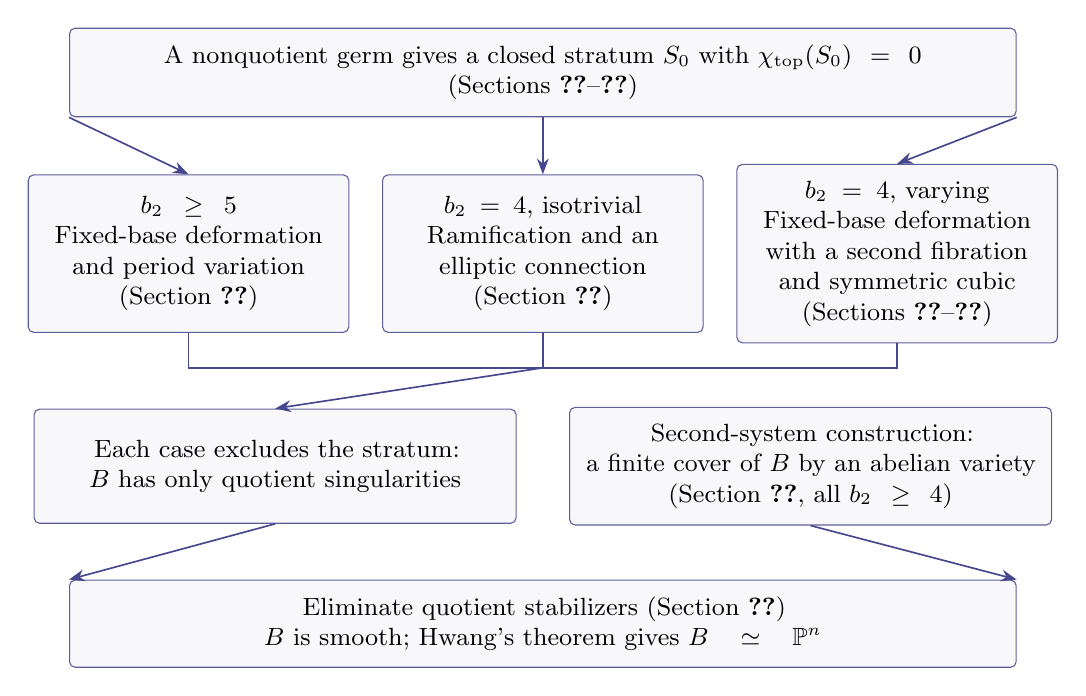
\begin{tikzpicture}[
  box/.style={draw=MidnightBlue!70,rounded corners=2pt,
    fill=MidnightBlue!3,align=center,inner sep=6pt,font=\small},
  line/.style={semithick,draw=MidnightBlue!80},
  arr/.style={line,-{Stealth[length=2mm]}}]
\node[box,text width=11.6cm] (zero) at (0,0)
  {A nonquotient germ gives a closed stratum \(S_0\) with
   \(\chi_{\mathrm{top}}(S_0)=0\)\\
   (Sections~\ref{sec:local-tensor}--\ref{sec:euler})};
\node[box,text width=3.65cm,minimum height=2cm] (large) at (-4.5,-2.3)
  {\(b_2\geq5\)\\Fixed-base deformation\\and period variation\\
   (Section~\ref{sec:deformation})};
\node[box,text width=3.65cm,minimum height=2cm] (iso) at (0,-2.3)
  {\(b_2=4\), isotrivial\\Ramification and an\\elliptic connection\\
   (Section~\ref{sec:isotrivial})};
\node[box,text width=3.65cm,minimum height=2cm] (vary) at (4.5,-2.3)
  {\(b_2=4\), varying\\Fixed-base deformation\\with a second fibration\\and symmetric cubic\\
   (Sections~\ref{sec:second-system}--\ref{sec:variation})};
\node[box,text width=5.7cm,minimum height=1.45cm] (quot) at (-3.4,-5)
  {Each case excludes the stratum:\\
   \(B\) has only quotient singularities};
\node[box,text width=5.7cm,minimum height=1.45cm] (cover) at (3.4,-5)
  {Second-system construction:\\a finite cover of \(B\) by an abelian variety\\
   (Section~\ref{sec:second-system}, all \(b_2\geq4\))};
\node[box,text width=11.6cm] (smooth) at (0,-7)
  {Eliminate quotient stabilizers (Section~\ref{sec:quotient})\\
   \(B\) is smooth; Hwang's theorem gives \(B\simeq\PP^n\)};
\draw[arr] (zero.south west)--(large.north);
\draw[arr] (zero.south)--(iso.north);
\draw[arr] (zero.south east)--(vary.north);
\draw[line] (large.south)--(-4.5,-3.75)--(0,-3.75);
\draw[line] (iso.south)--(0,-3.75);
\draw[line] (vary.south)--(4.5,-3.75)--(0,-3.75);
\draw[arr] (0,-3.75)--(quot.north);
\draw[arr] (quot.south)--(smooth.north west);
\draw[arr] (cover.south)--(smooth.north east);
\end{tikzpicture}
\caption{The first stage rules out a nonquotient germ in three cases.
The second uses both quotient singularities and a finite cover by an
abelian variety.}
\label{fig:proof}
\end{figure}

\FloatBarrier
\section{Notation and global inputs}\label{sec:setup}

All spaces are over $\C$ unless a reduction to positive characteristic
is specified. An irreducible holomorphic symplectic manifold is
abbreviated IHS. Write $q=q_X$ for the Beauville--Bogomolov--Fujiki
quadratic form, and $(\,\cdot\,,\,\cdot\,)$ for its associated
bilinear form. We also write $q(x,y)=(x,y)$, so that $q(x)=q(x,x)$.
We use the integral normalization; its real signature is
$(3,b_2(X)-3)$.

Choose a very ample line bundle $H$ on $B$, and set
\[
                         e=c_1(f^*H).
\]
For a coherent sheaf $M$ on a normal space, $M^{**}$ is its
reflexive hull. In particular,
$\Omega_B^{[j]}=(\bigwedge^j\Omega_B^1)^{**}$.
Reflexive tensor operations are always explicitly interpreted by
taking this hull. An associated map of a semiample line bundle is
replaced by its Stein factorization.

\begin{proposition}[Background for the given fibration]
\label{prop:background}
In the setting of Theorem~\ref{thm:main}, the following hold.
\begin{enumerate}
\item $X$ is projective, $e\neq0$ is nef and $q(e)=0$.
The base is $\Q$-factorial and klt, has Picard number one,
and $-K_B$ is ample as a $\Q$-Cartier divisor.
A smooth fiber is an abelian variety after choosing an origin.
\item There are reflexive identifications
\[
                  R^j f_*\cO_X\simeq\Omega_B^{[j]}.
\]
For every integral Weil divisor $A$ ample as a $\Q$-divisor,
\[
 H^i\!\left(B,
       (\Omega_B^{[j]}\otimes\cO_B(A))^{**}\right)=0
                       \quad(i>0,\ j>0).
\]
The reflexivity assertion also applies locally to the projective
equidimensional fibrations with connected fibers, smooth source \(Z\)
satisfying \(\omega_Z\simeq\cO_Z\), and normal Cohen--Macaulay
\(\Q\)-Gorenstein target that occur below.
\item The rational intersection cohomology of $B$ has the Betti
numbers of $\PP^n$, and the restriction of $H^2(X,\Q)$ to a
smooth fiber has one-dimensional image.
\item If $B$ is smooth, then $B\simeq\PP^n$.
\end{enumerate}
\end{proposition}

\begin{proof}
Relative ampleness and projectivity of $B$ make $X$ Moishezon;
as $X$ is Kähler, it is projective. Equivalently, a sufficiently
positive twist of a relative polarization by a base polarization
is ample. The structure statements in (1) are the fibration
theorems of Matsushita
\cite{Matsushita1999,Matsushita2001}.
The pullback of $H$ is nef and nonzero. Its $(2n)$-th power is
zero because $\dim B=n$, so Fujiki's relation gives $q(e)=0$.

For (2), Ou's Proposition~3.6 gives the reflexive cotangent
identifications for the given projective equidimensional Lagrangian
fibration, extending the symplectic differential identification of
Matsushita \cite{Matsushita2005,Ou2019}. Ou's Theorem~1.3 is the separate
local reflexivity result, and Theorem~1.4 gives the vanishing
\cite{Ou2019}.
The target hypotheses hold because klt spaces are
Cohen--Macaulay \cite[Theorem~11.1(2), Corollaries~11.9 and~11.14]{Kollar1997}
and $K_B$ is $\Q$-Cartier.
The cited reflexivity theorem has arbitrary-dimensional scope.
The higher-cohomology and fiber-restriction statements in (3)
are \cite[Theorem~0.4]{ShenYin2022}.
Statement (4) is Hwang's theorem \cite[Theorem~1.2]{Hwang2008}.
\end{proof}

Fix once and for all degreewise global isomorphisms
\[
 \phi_j:R^j f_*\cO_X\xrightarrow{\ \sim\ }\Omega_B^{[j]}
                  \qquad(0\leq j\leq n),
\]
with \(\phi_0\) the unit identification \(f_*\cO_X=\cO_B\).
The later normalized-chart constructions use the restrictions of these
same maps to \(B_{\mathrm{reg}}\); Proposition~\ref{str:direct-images}
constructs their compatible reflexive extensions on the charts.

We use intersection cohomology in Proposition~\ref{prop:background}
until rational smoothness has been proved in
Proposition~\ref{loc:rational-smoothness}, which then identifies it with
ordinary rational cohomology.

\begin{corollary}\label{cor:tangent-rigidity}
If $n>1$, then $H^1(B,T_B)=0$.
\end{corollary}
\begin{proof}
On the smooth locus, contraction identifies
$T_B$ with $\Omega_B^{n-1}\otimes\cO_B(-K_B)$.
Both sides extend reflexively, so
\[
 T_B\simeq
  (\Omega_B^{[n-1]}\otimes\cO_B(-K_B))^{**}.
\]
Apply Proposition~\ref{prop:background}(2), since $n-1>0$.
\end{proof}

The following elementary observation also appears in
\cite[Lemma~3.1]{GrebLehn2014}.

\begin{lemma}\label{lem:betti-bound}
One has $b_2(X)\geq4$.
\end{lemma}
\begin{proof}
Let $h$ be an ample class. Then $(h,e)>0$ and $q(e)=0$, so
$\langle h,e\rangle_{\R}$ is a hyperbolic plane.
It is perpendicular to the positive real plane generated by
$\operatorname{Re}\sigma$ and $\operatorname{Im}\sigma$.
These four independent real directions give the assertion.
\end{proof}

For a compact Kähler manifold $Y$, write $\mathcal K_Y$ for its
Kähler cone in $H^{1,1}(Y,\R)$.

\begin{theorem}[Strong hyperkähler SYZ, companion input]
\label{thm:strong-syz}
Let $Y$ be a compact IHS Kähler manifold of dimension $2m$.
If a holomorphic line bundle $L$ satisfies
\[
 c_1(L)\neq0,\qquad
 c_1(L)\in\overline{\mathcal K_Y},\qquad
 q_Y(c_1(L))=0,
\]
then a positive tensor power of $L$ is generated by its global
sections. Its associated map with connected fibers has a normal
projective base of dimension $m$. Every component of every fiber
has dimension $m$ and is Lagrangian.
\end{theorem}

This is Theorem~1.1 of the companion \cite{StrongSYZ2026}; it has no
restriction on \(b_2(Y)\), \(m\), or deformation type. The hypothesis
\(b_2\geq5\) in that manuscript belongs to its separate finiteness
Corollary~1.2. Section~\ref{sec:second-system} applies the theorem to a
second nonzero integral nef isotropic class on an actual projective
deformation. The class is of type \((1,1)\), so the exponential sequence
supplies its holomorphic line bundle.

\paragraph{Reduction to smoothness.}
For $n=1$, normality makes $B$ a smooth curve, and
Proposition~\ref{prop:background}(4) proves the result.
Henceforth $n>1$. It suffices to prove that $B$ is smooth.
Proposition~\ref{def:fixed-base} later supplies proper holomorphic
fibrations over this same \(B\) throughout the nearby \(e\)-Hodge locus.
The original fibration and the projective deformation carrying two
Lagrangian systems have the stronger projectivity used in their respective
arguments.

\paragraph{The Euler obstruction.}
The first stage has a specific numerical target. If \(B\) has a
nonquotient germ, Sections~\ref{sec:local-tensor}--\ref{sec:stratum}
produce a nonempty closed irreducible normal projective stratum
\(S_0\subset B\) of dimension \(d<n\). Proposition~\ref{eu:euler-zero},
proved through Sections~\ref{sec:base-change}--\ref{sec:euler}, establishes
\[
                         \chi_{\mathrm{top}}(S_0)=0.
\]
Here \(\chi_{\mathrm{top}}\) is the ordinary topological Euler
characteristic of the coarse space. The local construction also gives a
smooth stack \(\cS\) above \(S_0\); we write \(c=n-d>0\).
Its finite stabilizers, including those acting trivially on the stratum,
are retained in the calculations. In characteristic \(p\), their orders
are chosen prime to \(p\). The later geometric arguments will contradict
this Euler equality when \(b_2(X)\geq5\) and in the isotrivial and varying
cases with \(b_2(X)=4\).

\section{Finite local covers and cotangent tensors}
\label{loc:section}
\label{sec:local-tensor}

We first establish three geometric facts about the base germs: finite
smooth domination, rational smoothness, and the existence of maximal
finite quasi-\'etale charts.  The normalized source over such a chart
will also provide the direct-image and descent maps used later.
We then study reflexive cotangent tensors on one maximal chart through
a residual trace category.  Its tensor group acts on the fiber spaces
of that category.  The obstruction to a holomorphic connection
identifies the nontrivial irreducible summands of the cotangent fiber
representation as standard blocks for special linear and symplectic groups,
which enter the Euler calculation in
Section~\ref{sec:euler}.  A finite
map between normal spaces is called \emph{quasi-\'etale} if it is
\'etale outside a subset of codimension at least two in the target.
The geometric tensor argument uses complex analytic local rings of the
maximal charts; they are excellent and henselian, with residue field
$\C$.  The trace and split-lifting lemmas are stated for general normal
henselian local rings as well, so that they apply after completion.
Reflexive pullback means pullback followed by double dual.

\begin{lemma}[Finite smooth domination]
\label{loc:smooth-domination}
Every point of $B$ has an algebraic neighborhood, after an \'etale
base change if necessary, admitting a finite surjection from a smooth
variety of dimension $n$.  In particular, every analytic germ of $B$
is finitely dominated by a smooth germ of the same dimension.
Every such germ is analytically $\Q$-factorial.
\end{lemma}

\begin{proof}
Fix $b\in B$.  Choose sufficiently positive very ample divisors on the
smooth projective variety $X$.  By Bertini, a general intersection of
$n$ of them is smooth of dimension $n$.  They may simultaneously be
chosen so that their intersection with each component of $f^{-1}(b)$
is zero-dimensional and nonempty: the fiber has finitely many
components, all of dimension $n$, and successive general hyperplanes
cut each of them properly.  Denote the resulting smooth intersection
by $Y$.  The proper map $Y\to B$ is quasi-finite over $b$, and hence
finite over a neighborhood of $b$.  Its image contains that
neighborhood, by properness and the dimension theorem.  A local
branch at a point of $Y$ over $b$ gives the asserted finite map of
analytic germs.  If an individual algebraic branch is required, split
the finite algebra over the henselization and descend the corresponding
idempotents to an \'etale neighborhood.

Let $\pi:(Y,y)\to (B,b)$ be a finite dominating smooth germ, of degree
$m$, and let $D$ be a Weil divisor on $(B,b)$.  Pullback of Weil
divisors under a finite map is defined by the ramification indices of
the discrete valuations at prime divisors.  The divisor $\pi^*D$ is
principal on the smooth local germ, say $\operatorname{div}(g)$.
The valuation formula for the field norm gives
\[
 \operatorname{div}\bigl(\operatorname{Nm}_{\C(Y)/\C(B)}g\bigr)
       =\pi_*\pi^*D=mD.
\]
Thus $mD$ is Cartier.  The argument is analytic and therefore proves
the stronger local assertion needed later, rather than merely
algebraic $\Q$-factoriality.
\end{proof}

\begin{proposition}[Rational smoothness]
\label{loc:rational-smoothness}
The space $B$ is an oriented rational homology manifold of real
dimension $2n$.  Its rational intersection complex is
$\Q_B[n]$.  Consequently its ordinary rational cohomology has the
Betti numbers of $\PP^n$.  The local rational homology-manifold
assertion holds for every normal germ finitely dominated by a smooth
germ, in particular for the maximal charts constructed below.
\end{proposition}

\begin{proof}
We explain the trace at a branch point.  For a finite surjection
$\pi:Y\to U$ from a smooth $n$-fold to a normal connected
neighborhood, let $m_y$ be the local generic degree of the branch at
$y$.  A section $a$ of $\pi_*\Q_Y$ is locally constant on $Y$.
Set
\[
 \operatorname{Tr}_{\pi}(a)(b)
       =\sum_{y\in\pi^{-1}(b)}m_y a(y).
\]
This is locally constant.  Indeed, choose disjoint neighborhoods of
the finitely many points above $b$.  After shrinking downstairs, the
sum of the local generic degrees in each of these neighborhoods is
constant: it equals the degree over the common unbranched dense open
of the locally irreducible normal base.  The value of $a$ is constant
on each chosen neighborhood.  This proves the assertion and shows
that the trace is a morphism of sheaves.  Its composite with the
constant-section inclusion $\Q_U\to\pi_*\Q_Y$ is multiplication by
$\deg\pi$.  Therefore $\Q_U$ is a direct summand of
$\pi_*\Q_Y$.

Proper base change and the finiteness of the fibers give
$R^j\pi_*\Q_Y=0$ for $j>0$.  Applying the point costalk at $b$ to
the preceding direct summand, and using proper base change for
costalks, exhibits
\[
 H^k_{\{b\}}(U,\Q)
       \quad\text{as a direct summand of}\quad
 \bigoplus_{y\in\pi^{-1}(b)}H^k_{\{y\}}(Y,\Q).
\]
The latter group is zero unless $k=2n$.  The top local group on the
normal, hence locally irreducible, complex analytic germ $U$ is
one-dimensional: the complex orientation gives its fundamental
class, and the top fundamental cycles of a pure analytic germ are
indexed by its local irreducible components
\cite[Section~1.4, Theorem~3.2, Section~3.3 and Lemma~4.3]{BorelHaefliger1961}.
Here fundamental classes are taken in Borel--Moore homology of
representatives and passed to local groups. Equivalently, this
follows from an analytic triangulation and the oriented top strata.
Thus the costalk of $\Q_U$ is exactly $\Q[-2n]$ at every point,
with the compatible complex orientation.  This is the rational
homology-manifold assertion and identifies the intersection complex
with the shifted constant sheaf
\cite[Theorem~1.1(1)$\Leftrightarrow$(4)]{Massey2005}.
The final claim now follows from
the base-cohomology theorem recalled in
Proposition~\ref{prop:background}; the passage from intersection to
ordinary cohomology has been justified before using it.
\end{proof}

\begin{proposition}[Maximal quasi-\'etale charts and normalized source charts]
\label{loc:maximal-charts}
Every pointed germ $(B,b)$ has a connected finite normal Galois
quasi-\'etale cover $(C,c)$ which dominates every connected finite
quasi-\'etale cover of that germ.  The chart $(C,c)$ is klt, is
finitely dominated by a smooth germ, and has no nontrivial connected
finite quasi-\'etale cover.  The finite diagrams can be defined over
an algebraic \'etale neighborhood of $b$.

More generally, let $U\to B$ be an integral separated \'etale algebraic
neighborhood and let $\pi:C\to U$ be an integral finite normal
quasi-\'etale cover.  Put $X_U=X\times_B U$.  The base change
$X_U\times_U C$ has a unique irreducible component dominating $C$;
let $Z$ be its normalization and $h:Z\to C$ its structure map.
Then $h$ is projective and equidimensional of relative dimension $n$,
has connected fibers, and satisfies $h_*\cO_Z=\cO_C$.  The finite map
$p:Z\to X_U$ is \'etale.  Consequently $Z$ is smooth, the pullback of
the symplectic form on $X$ is symplectic on $Z$, its canonical bundle is
trivial, and the fibers of $h$ are Lagrangian.  If $\pi$ is Galois with
group $\Gamma$, then $p$ is a $\Gamma$-torsor.  Ordinary \'etale base
change on $C$ preserves projectivity, equidimensionality, connected
fibers, the equality $h_*\cO_Z=\cO_C$, and the smooth symplectic source.
The torsor in the statement belongs to the original finite chart.
\end{proposition}

\begin{proof}
Work first over the strict henselization of the algebraic germ and
choose a finite smooth slice as in
Lemma~\ref{loc:smooth-domination}.  Choose a connected local factor
of its finite algebra, with fraction field $L$ over the base field
$K$.  If $K'/K$ defines a finite quasi-\'etale normal cover, the
normalization of its pullback to this slice is unramified outside a
set of codimension at least two.  Finiteness preserves that
codimension bound.  The source of the normalized map is normal and
the target is regular, so purity of the branch locus
\cite[Tag 0BMB]{StacksProject} makes the map \'etale everywhere.
A connected finite \'etale cover of a strictly henselian regular
local scheme is trivial.  A component of the split pullback
therefore embeds $K'$ into $L$ over $K$.

Let $M/K$ be a finite Galois closure of $L/K$, let $W$ be the
normalization of the base in $M$, and write $\Gamma$ for its Galois
group.  Normalizations are finite by excellence.  Let $H\lhd\Gamma$
be the normal subgroup generated by the inertia groups of all prime
divisors of $W$.  The finite quotient $C=W/H$ is unramified over
every prime divisor of the normal base and hence is quasi-\'etale.
Conversely, an intermediate extension which is quasi-\'etale has
trivial divisorial inertia; its defining subgroup contains every
conjugate of each inertia group, and hence contains $H$.  Every
quasi-\'etale cover is consequently dominated by $C$.  A further
quasi-\'etale cover of $C$ would give one of the base and is therefore
trivial.  Applying the same split-pullback argument to $C$ shows
that it too is finitely dominated by the smooth slice.

All finite algebras, group actions, quotient maps and their
identities descend from the strict henselization to an \'etale
neighborhood.  Shrinking removes branch divisors not meeting the
marked fiber.  This construction also gives the analytic maximum.
Indeed, the normalized pullback of any finite analytic
quasi-\'etale cover to the smooth germ is \'etale by analytic purity
and splits because a smooth germ is simply connected.  One may
also obtain this directly: a small smooth ball minus an analytic
set of complex codimension at least two is simply connected, by
general position for disks against a stratification; its finite
cover splits there, and normalization extends that splitting
uniquely.  The analytic cover is thus
an intermediate cover of the analytification of the same finite
Galois closure.  Finite normalizations and finite-group quotients
commute here with analytification; the local normal components and
their degrees agree.  The divisorial inertia groups through the
marked point are therefore the same in both constructions.  Finally
$C$ is klt.  Indeed, writing $\pi:C\to B$, we have
$K_C=\pi^*K_B$ in codimension one, and for a
divisorial valuation $E$ over $C$ restricting with ramification index
$r$ to a divisorial valuation $F$ over $B$, the canonical ramification
formula on normalized birational models gives
$A_C(E)=rA_B(F)$.  The latter is positive because $B$ is klt.

We prove the source assertions, including connectedness.  The connected
fibers of $f$ and normality of $B$ give $f_*\cO_X=\cO_B$ by Stein
factorization.  This equality persists after the flat base change to
$U$.  Let $K=\C(U)$, $L=\C(C)$, and let $F$ be the generic fiber of
$X_U\to U$.  Generic smoothness makes $F$ smooth.  Proper flat field
base change gives
\[
 H^0(F_{\overline K},\cO_{F_{\overline K}})=\overline K.
\]
Thus $F_{\overline K}$ is connected.  A connected smooth scheme over
an algebraically closed field is integral, since its irreducible
components are disjoint.  In this setting it is an abelian variety
after an origin is chosen, by Proposition~\ref{prop:background}.
In particular $F$ is geometrically integral, so $F_L$ is integral
and normal and has $H^0(F_L,\cO_{F_L})=L$.  This proves uniqueness of
the component dominating $C$ and identifies the generic fiber of its
normalization $Z$ with $F_L$.

The normalization is finite by excellence, so $h$ is projective.
Its Stein algebra $h_*\cO_Z$ is finite over $\cO_C$ and embeds in the
generic algebra $L$: a section on the integral space $Z$ is determined
by its restriction to the generic fiber.  Every such section is
integral over $\cO_C$; normality of $C$ therefore gives
$h_*\cO_Z=\cO_C$.  Stein factorization now gives connected fibers.
This part of the argument used only that $C\to U$ is finite and
dominant, with $C$ normal and integral.

Let $D\subset U$ have codimension at least two and contain the branch
locus of $\pi$.  Equidimensionality of $f$ gives
\[
 \dim f_U^{-1}(D)\leq\dim D+n\leq2n-2.
\]
The map $p$ is finite over the smooth space $X_U$ and is \'etale away
from $f_U^{-1}(D)$.  Purity makes it \'etale everywhere, so $Z$ is
smooth and carries the pulled-back symplectic form.  Each component of
a fiber of $h$ has dimension at most $n$, because its finite image lies
in a fiber of $f_U$.  The fiber dimension theorem gives the reverse
inequality.  Hence $h$ is equidimensional of relative dimension $n$;
the same finite images show that its fiber components are Lagrangian.
The symplectic form trivializes the canonical bundle of $Z$.

If $\pi$ is Galois, its deck action lifts to $Z$.  Over the dense
unbranched locus the map $p$ is a deck torsor.  Both sides of the torsor
map $\Gamma\times Z\to Z\times_{X_U}Z$ are finite \'etale over $Z$,
so their isomorphism on that dense locus extends over $Z$.  This proves
freeness of the action also over special fibers.  Subsequent \'etale
refinements of the object chart use ordinary base change of $h$ and
preserve its projectivity, equidimensionality, connected fibers and
smooth symplectic source.  The torsor descent is retained from the
finite chart before that refinement.
\end{proof}

\subsection{The trace quotient}

Fix a maximal chart and let $(R,\mathfrak m)$ be its analytic local
ring.  Put $V=\Omega_R^{[1]}$.  On reflexive modules we use
$M\mathbin{\widehat\otimes}N=(M\otimes_RN)^{**}$ and
$M^\vee=\Hom_R(M,R)$.  These are a symmetric rigid tensor product
and dual: on a common open set containing every point of codimension
one they are the ordinary bundle operations, and all identities
extend uniquely by reflexivity.  In particular the categorical trace
is the usual generic trace, which lies in $R$ by normality.  We use
the full additive, idempotent-complete tensor subcategory $\mathcal C$
generated by $V$ and $V^\vee$.  Every object in this subcategory is a vector
bundle on the smooth locus of the chart.

There are two uses of endomorphisms below.  The ordinary finite
$R$-algebra $A_M=\End_R(M)$ consists of morphisms of the module $M$.
The internal endomorphism object is
\[
 \underline{\End}(M)=M\widehat\otimes M^\vee.
\]
Its underlying reflexive module is canonically $\Hom_R(M,M)$: this is
the usual bundle identification in codimension one, extended
reflexively.  We use the underline when this module is a coefficient
object in $\mathcal C$, rather than the algebra of morphisms of $M$.

\begin{lemma}[The trace ideal is the Jacobson radical]
\label{loc:trace-radical}
Let $(R,\mathfrak m)$ be any noetherian normal henselian local
$\C$-algebra with residue field $\C$.  For finite reflexive modules
$M,N$, define
\[
 \mathcal R(M,N)=
 \{a\in\Hom_R(M,N):\tr(ba)\in\mathfrak m
                 \text{ for every }b\in\Hom_R(N,M)\}.
\]
These spaces form a tensor ideal.  For every $M$,
$\mathcal R(M,M)$ is the Jacobson radical of the finite
$R$-algebra $\End_R(M)$.  The quotient category is semisimple
abelian over $\C$, has finite-dimensional Hom spaces, and its
categorical dimensions are the positive integer ranks of its
nonzero objects.
\end{lemma}

\begin{proof}
Cyclicity of trace proves stability under composition.  Stability
under tensor product follows by taking a partial trace: for a map
$a:M\to N$ and a test map
$b:N\widehat\otimes P\to M\widehat\otimes P$, the trace of
$b(a\widehat\otimes\id_P)$ is the trace of $a$ composed with the
partial trace of $b$.  These formulas hold for bundles in codimension
one and therefore over $R$.  Duality is compatible with the same
ideal.

Write $A=A_M=\End_R(M)$ and $J=\rad A$.  The algebra $A$ is finite over
the henselian local ring $R$, so $\mathfrak m A\subset J$,
$A/J$ is a finite-dimensional semisimple $\C$-algebra, and
$J^q\subset\mathfrak m A$ for some $q$.  We recall why idempotents
lift in this setting.  First lift an idempotent through the nilpotent
radical of $A/\mathfrak m A$.  For an ensuing lift $a\in A$ of an
idempotent modulo $\mathfrak m A$, the commutative finite algebra
$R[a]$ splits into the factors supported at $0$ and $1$ in its
closed fiber by henselianity.  The resulting idempotent lifts the
given one.  Induction in complementary corners lifts an entire
orthogonal system.  Thus primitive idempotents of $A/J$ lift to
actual direct summands of $M$.

For $x\in J$, all sufficiently large powers $x^j$ belong to
$\mathfrak m A$, so their traces vanish modulo $\mathfrak m$.
The generic characteristic polynomial of $x$ has coefficients in
$R$: this is true at every height-one localization, where $M$ is
free, and $R$ is the intersection of those valuation rings.  If
$\lambda_1,\ldots,\lambda_r$ are the roots of its reduction over
$\C$, Newton identities give
$\sum_i\lambda_i^j=0$ for every sufficiently large $j$.
Grouping the distinct nonzero roots, a Vandermonde matrix applied to
consecutive such powers forces all their multiplicities to be zero.
There are consequently no nonzero roots, and $\tr(x)=0$ modulo
$\mathfrak m$.  The same holds for $yx$ for any $y\in A$, because
$J$ is an ideal.  Hence $J\subset\mathcal R(M,M)$.

The residual trace now descends to $A/J$.  On each simple block
$\operatorname{Mat}_t(\C)$ it is a scalar multiple of the ordinary
matrix trace, by cyclicity.  Evaluate it on a primitive diagonal
idempotent.  Its lift projects onto a nonzero reflexive direct
summand $M_0$, so the scalar is $\rk(M_0)>0$.  The trace pairing is
therefore nondegenerate on every block.  This proves the reverse
inclusion and the equality with $J$.

Apply the argument to finite direct sums of objects.  Their
endomorphism algebras in the quotient are semisimple matrix algebras,
and their primitive projectors lift.  In particular every object is
a finite sum of simple objects, distinct simple objects have no
morphisms, and the endomorphisms of each simple object are $\C$.
This also proves that the quotient is abelian and that all its exact
sequences split.  The ideal contains $\mathfrak m\Hom_R(M,N)$,
so its Hom spaces are finite-dimensional.  Finally the trace of the
identity is $\rk M$, as asserted.
\end{proof}

\begin{lemma}[Lifting split maps]
\label{loc:split-lift}
Over any ring in Lemma~\ref{loc:trace-radical},
if a morphism of reflexive modules becomes a split injection in the
trace quotient, it is already a split injection of reflexive modules.
An isomorphism in the quotient lifts to an isomorphism.  In
particular, an object is a sum of copies of the tensor unit in the
quotient if and only if its underlying module is free.
\end{lemma}

\begin{proof}
Let $a:M\to N$ and lift a left inverse in the quotient to
$b:N\to M$.  Then $ba=\id_M+r$ with $r\in\rad\End_R(M)$,
so $ba$ is invertible.  Replacing $b$ by $(ba)^{-1}b$ gives an
actual left inverse.  If the quotient map is an isomorphism, apply
the same argument to both composites of lifts of it and its inverse;
the lift is an isomorphism.  Apply this to an isomorphism with $R^r$
for the final statement.
\end{proof}

Return now to the analytic maximal chart and the category $\mathcal C$
fixed above.

\begin{proposition}[The residual tensor group]
\label{loc:tannakian}
The residual category $\overline{\mathcal C}=\mathcal C/\mathcal R$
admits a fiber functor $\omega$ to complex vector spaces.  For a choice
of $\omega$, tensor reconstruction identifies it with
$\operatorname{Rep}_{\C}(G)$, where
$G=\Aut^\otimes(\omega)$ is a reductive algebraic subgroup of
$\operatorname{GL}(V_{\mathrm{fib}})$ and
$V_{\mathrm{fib}}=\omega(\overline V)$.  This representation is
faithful and has dimension $n$.
\end{proposition}

\begin{proof}
Lemma~\ref{loc:trace-radical} gives an abelian rigid symmetric
$\C$-linear category with $\End({\bf1})=\C$.  Tensor product is
exact because every exact sequence splits.  For an object of rank
$r$, its $(r+1)$st exterior power is zero: it is zero on the common
bundle locus and hence its reflexive extension is zero.  Deligne's
criterion \cite[Theorem 7.1]{Deligne1990} therefore applies.  The
category is tensor-generated by one object; Deligne's
Corollary~6.20 supplies a fiber functor over a finite extension of
$\C$, hence over $\C$ itself.  Tensor reconstruction gives the
stated group.  A tensor generator makes it an algebraic subgroup of
its general linear group, and semisimplicity of the representation
category makes it reductive in characteristic zero.  The fiber
dimension equals the categorical dimension, namely $\rk V=n$.
\end{proof}

We call $G$ the residual tensor group of the chosen fiber functor.
Its representations are the fiber spaces of $\overline{\mathcal C}$.
Finite deck groups, denoted by $\Gamma$, act on the geometric charts.
For example, if $M_{\mathrm{fib}}=\omega(\overline M)$, then
\[
 \omega\bigl(\overline{\underline{\End}(M)}\bigr)
       =\End_{\C}(M_{\mathrm{fib}}),\qquad
 \End_{\overline{\mathcal C}}(\overline M)
       =\End_G(M_{\mathrm{fib}}).
\]
The first space is the full internal coefficient representation, with
the conjugation action; the second is its space of invariant vectors.

\subsection{Connections before and after the trace quotient}

For an object $M$ let $M_U$ be its vector bundle on the smooth locus
$U$ of a sufficiently small representative of the chart.  Its
ordinary Atiyah class \cite{Atiyah1957} is
\[
 a(M_U)\in H^1\bigl(U,\Omega_U^1\otimes\End(M_U)\bigr).
\]
It vanishes precisely when $M_U$ has a holomorphic connection;
integrability is not part of this assertion.  We take the direct
limit over shrinking representatives when discussing this class on
a germ.  All cohomology in the following lemmas is this ordinary
sheaf cohomology.

\begin{lemma}[A connection gives freeness on a maximal chart]
\label{loc:connection-free}
If $a(M_U)=0$, then $M$ is a free $R$-module.
\end{lemma}

\begin{proof}
Pull a connection on $M_U$ back to a finite smooth dominating germ
$\pi:(Y,y)\to(C,c)$.  The complement of $\pi^{-1}(U)$ has
codimension at least two.  On $Y$ let
$F=(\pi^*M)^{**}$.  In local smooth coordinates each coefficient
of the connection extends across that complement by the Hartogs
property of $F$.  Its target $F\otimes\Omega_Y^1$ is reflexive
because $\Omega_Y^1$ is locally free.  Thus the connection extends
to $F$ and still satisfies Leibniz's rule.

Here is the elementary freeness argument, which does not require a
flat connection.  For a coordinate derivation $\partial$, choose a
presentation of $F$ and lift the operator $\nabla_{\partial}$ to
the free module of generators.  If $A$ is the corresponding matrix
on generators and $P$ a matrix of relations, stability of the
relations gives a matrix $Q$ with
\[
                 \partial P+AP=PQ.
\]
The derivative of every minor of $P$ is therefore a linear
combination of minors of the same size.  Each Fitting ideal of $F$
is stable under every coordinate derivation.  A nonzero ideal in a
smooth characteristic-zero local ring with this property is the
unit ideal: repeatedly differentiating a nonzero element of minimal
order produces an element with nonzero constant term.  If $r$ is
the generic rank of $F$, its $r$th Fitting ideal is nonzero and hence
is the unit ideal.  Thus $F$ is generated by $r$ elements.  The
resulting surjection from a free module of rank $r$ has a torsion
kernel, which is zero because it is a submodule of a free module
over a domain.  This proves that $F$ is free.

Take a normal Galois closure $W\to C$ of $Y\to C$, with group
$\Gamma$.  Its normal domain is local over the henselian germ,
so the whole group fixes the unique marked point.  The
reflexive pullback $P$ of $M$ to $W$ is free: it agrees in
codimension one with the pullback of the free module $F$, and both
reflexive extensions agree.  It has its natural semilinear
$\Gamma$-action.  At a prime divisor, divisorial inertia acts
trivially on its restriction to that divisor, because there $P$
is the ordinary pullback of a bundle from $C$.  The same inertia
therefore acts trivially on the fiber of $P$ at the marked point.
To see the last specialization explicitly, for an inertia element
of order $m$, restrict $P$ to its fixed locus and apply the
idempotents
\[
       \frac1m\sum_{j=0}^{m-1}\zeta^{-j}g^j.
\]
Their ranks are locally constant.  On the divisor all nonidentity
eigenvalues have rank zero, hence they have rank zero at its
specialization to the marked point as well.

Since $C$ has no further quasi-\'etale cover, these inertia groups
normally generate $\Gamma$, by the construction in
Proposition~\ref{loc:maximal-charts}.  The action on the marked
fiber of $P$ is consequently trivial.  Lift a basis of that fiber
to sections of $P$ and average over $\Gamma$.  The averaged
sections still lift the basis and hence, by Nakayama, form a basis
of the free module $P$.  This basis is $\Gamma$-invariant.
The invariant basis identifies $P^\Gamma$ with $R^r$, because the
invariants of the normal cover ring are $R$.  Thus $P^\Gamma$ is
reflexive.  The natural map $M\to P^\Gamma$ is an isomorphism in
codimension one by ordinary finite descent for the pullback of a
bundle.  Both modules are reflexive, so this isomorphism extends over
the normal germ.  Hence $M=P^\Gamma$ is free, as claimed.
\end{proof}

\begin{lemma}[Tensor tests for the ordinary Atiyah class]
\label{loc:atiyah-tests}
Let $M$ be an object, and let $t_j$ be actual sections of finitely
many functorial mixed tensor powers $T_j(M)$ of $M$ and $M^\vee$ on
the chart.  Direct sums and the usual symmetric or alternating
projectors may be used; each construction carries the natural action
of every endomorphism of $M$.  Put $Q=\bigoplus_jT_j(M)$ and define
\[
 \Phi_M:\underline{\End}(M)\longrightarrow Q,
       \qquad A\longmapsto(A\cdot t_j)_j
\]
by the infinitesimal tensor action.  The coefficient map for the
Atiyah class is the morphism in $\mathcal C$
\begin{equation}\label{loc:psi-coefficient}
 \Psi_M=\id_V\widehat\otimes\Phi_M:
 V\widehat\otimes\underline{\End}(M)
       \longrightarrow V\widehat\otimes Q.
\end{equation}
On the smooth locus its ordinary bundle restriction satisfies
$(\Psi_{M,U})_*a(M_U)=0$ in $H^1(U,(V\widehat\otimes Q)_U)$.
If $\overline{\Psi_M}$ is injective in $\overline{\mathcal C}$, then
$a(M_U)=0$.
\end{lemma}

\begin{proof}
The natural tensor action defining $\Phi_M$ is a bundle map on $U$;
its reflexive extension is the displayed morphism in $\mathcal C$.
Choose local connections $\nabla_\alpha$ on $M_U$.
Their differences represent $a(M_U)$.  On $T_j(M_U)$ the
corresponding differences are the infinitesimal tensor actions of
$\nabla_\alpha-\nabla_\beta$.  Evaluating on the global section
$t_j$ gives the coboundary of the local sections
$\nabla_\alpha t_j$.  This proves the asserted vanishing after
restricting \eqref{loc:psi-coefficient} to bundles on $U$ and taking
ordinary $H^1$.

An injection in the semisimple quotient has a left inverse there.
Lemma~\ref{loc:split-lift} lifts it to an actual left inverse
between reflexive coefficient modules.  Restriction to $U$ gives
a split map of bundles, which induces an injection on ordinary
$H^1$.  Its kernel contains $a(M_U)$, so that class is zero.
The argument uses only that the individual $t_j$ are actual
sections.  No algebraic identities among their images in the
quotient need hold for the chosen lifts.
\end{proof}

\begin{proposition}[Connectedness and semisimplicity]
\label{loc:connected-semisimple}
The reductive group $G$ of Proposition~\ref{loc:tannakian} is
connected and semisimple.
\end{proposition}

\begin{proof}
For a reductive subgroup of a general linear group, the invariant
mixed tensors have that subgroup as their simultaneous pointwise
stabilizer.  Indeed, projectors onto direct summands and all maps
between tensor constructions are themselves such tensors.
Preserving them is precisely the condition to give a tensor
automorphism of the forgetful functor, and tensor reconstruction
identifies those automorphisms with the group.  Differentiating,
its Lie algebra is the common kernel of the infinitesimal
tensor-action maps.  Since the endomorphism space is
finite-dimensional, finitely many tensors suffice for this last
kernel.

Suppose a representation $N$ of $G$ has finite image.  Realize it
as a direct summand of tensor constructions in
$V_{\mathrm{fib}}$, and lift its projector to obtain an actual
module $M$.  Choose finitely many invariant mixed tensors of $N$
whose infinitesimal stabilizer is the zero Lie algebra.  By the
definition of the quotient Hom spaces these tensors lift to actual
maps from $R$, hence to actual sections on the chart.  The map
$\omega(\overline{\Phi_M})$ of Lemma~\ref{loc:atiyah-tests} has as
its kernel this infinitesimal stabilizer inside the full space
$\End_{\C}(N)$, and is therefore injective.  Thus
$\overline{\Phi_M}$ is injective.  Tensoring it with $\overline V$
preserves injectivity, so $\overline{\Psi_M}$ is injective and that
lemma and Lemma~\ref{loc:connection-free} make $M$ free.
Therefore $N$ is trivial.  The regular representation of the
finite component group $G/G^\circ$ is one such representation.
It is trivial only if that component group is trivial.  Hence $G$
is connected.

A character of $G$ corresponds to a rank-one reflexive module on
the chart.  By analytic $\Q$-factoriality some positive reflexive
tensor power of that module is free.  Thus the character has
finite order.  A connected algebraic group has no nontrivial
finite-image character.  The character group of $G$ is therefore
zero.  For a connected reductive group its quotient by the derived
group is a torus, whose characters detect it; that torus must be
trivial.  Thus $G$ is semisimple.
\end{proof}

\subsection{The prolongation forced by a nontrivial cotangent block}

For a vector space $T$ and a Lie subalgebra
$\mathfrak h\subset\End(T)$, set
\[
 \mathfrak h^{(1)}=
 \{A\in\Sym^2T^*\otimes T:
                      A(x,{-})\in\mathfrak h\text{ for every }x\in T\}.
\]
For a reflexive module $M$, let $\Sym^{[2]}M$ denote the image of the symmetric idempotent
$(1+\tau)/2$ on $M\widehat\otimes M$.  It is a reflexive direct
summand and restricts to the usual symmetric square on the bundle
locus.  For a block $V_i$ below with fiber
$L_i=\omega(\overline V_i)$ and $T_i=L_i^\vee$, the fiber of its
coefficient module is
\[
 \omega\bigl(\overline{\Sym^{[2]}V_i\widehat\otimes V_i^\vee}\bigr)
       =\Sym^2L_i\otimes L_i^\vee
       =\Sym^2T_i^*\otimes T_i.
\]
The intersection defining a prolongation will be taken in this fiber
space.
We use Lie's triangularization theorem and complete reducibility
for finite-dimensional complex representations, in the forms
\cite[Theorem 2.2(2), Corollary 2.2(2), Theorem 2.9]{Cap2016}.
The prolongation spaces belong to the Singer--Sternberg framework
\cite{SingerSternberg1965}. The infinite-type rank-one criterion is due
to Guillemin--Quillen--Sternberg \cite{GuilleminQuillenSternberg1967};
see also the proof and attribution in
\cite[Section~2.2 and Theorem~2.3]{OttazziWarhurst2011}.
We give the prolongation argument in full, including the separate
semisimple-irreducible step from nonzero first prolongation to infinite
type.

\begin{lemma}[One-block connection obstruction]
\label{loc:block-obstruction}
Lift a decomposition of $V_{\mathrm{fib}}$ into irreducible
$G$-modules to a decomposition $V=\bigoplus_iV_i$ of reflexive
modules.  Let
\[
 \mathfrak h_i=
    \mathfrak g\cap\End(V_{i,\mathrm{fib}})
       \subset\End(V_{\mathrm{fib}}),
       \qquad\mathfrak g=\operatorname{Lie}(G),
\]
where the endomorphisms in this intersection are zero on every
other block.  Regard $\mathfrak h_i$ on
$T_i=V_{i,\mathrm{fib}}^\vee$ by the dual action.  If
$\mathfrak h_i^{(1)}=0$, then $V_i$ is free.  Consequently every
nontrivial irreducible block has
$\mathfrak h_i^{(1)}\ne0$.
\end{lemma}

\begin{proof}
Local coordinate connections on $\Omega_U^1$ are torsion-free.
Their differences show that $a(V_U)$ belongs to the direct summand
\[
 H^1\bigl(U,\Sym^2V_U\otimes V_U^\vee\bigr)
       \subset H^1\bigl(U,V_U\otimes\End(V_U)\bigr).
\]
On the other hand, choose local connections preserving the actual
splitting $V_U=\bigoplus_i(V_i)_U$.  The off-diagonal
endomorphism components of the same cohomology class are zero.
These two conditions imply
\begin{equation}
 a(V_U)=\sum_i a_i,\qquad
 a_i\in H^1\bigl(U,\Sym^2(V_i)_U\otimes(V_i)_U^\vee\bigr).
 \label{loc:diagonal-atiyah}
\end{equation}
Here is the index check.  Block preservation allows only
coefficients $V_a\otimes V_b\otimes V_b^\vee$.  Symmetry
interchanges the first two covariant slots.  If $a\ne b$, its
image is an off-diagonal coefficient
$V_b\otimes V_a\otimes V_b^\vee$, whose class is zero.
Because these are actual direct sums of bundles, the original
mixed component is also zero.  This leaves precisely the terms in
\eqref{loc:diagonal-atiyah}.  In particular $a_i$ is the class
$a((V_i)_U)$ under the indicated inclusion of its coefficients.

Choose lifts $t_j$ of finitely many $G$-invariant tensors in natural
mixed powers of $V_{\mathrm{fib}}$ cutting out $\mathfrak g$
infinitesimally.  Use them to define $Q$ and $\Phi_V$ as in
Lemma~\ref{loc:atiyah-tests}.  For the $i$th block set
\[
 S_i=\Sym^{[2]}V_i\widehat\otimes V_i^\vee.
\]
The symmetric inclusion in the first two slots, followed by the
diagonal inclusion of the $i$th endomorphism block, gives
\[
 \jmath_i:S_i\longrightarrow
          V_i\widehat\otimes\underline{\End}(V).
\]
The required one-block coefficient map is
\begin{equation}\label{loc:kappa-coefficient}
 \kappa_i=(\id_{V_i}\widehat\otimes\Phi_V)\circ\jmath_i:
 S_i\longrightarrow V_i\widehat\otimes Q.
\end{equation}
On $U$ the source of this map is
$\Sym^2(V_i)_U\otimes(V_i)_U^\vee$.  Projecting the first slot of
$(\Psi_{V,U})_*a(V_U)=0$ onto $(V_i)_U$ and using
\eqref{loc:diagonal-atiyah} gives
$(\kappa_{i,U})_*a_i=0$ in ordinary $H^1$.

Write $L=V_{\mathrm{fib}}$ and $L_i=V_{i,\mathrm{fib}}$.
The kernel of $\omega(\overline{\Phi_V})$ is $\mathfrak g$ inside
$\End_{\C}(L)$.  Hence the fiber kernel of
\eqref{loc:kappa-coefficient} is the explicit intersection
\begin{equation}\label{loc:kappa-kernel}
 \ker\omega(\overline{\kappa_i})=
 \bigl(\Sym^2L_i\otimes L_i^\vee\bigr)
          \cap\bigl(L_i\otimes\mathfrak g\bigr)
       \quad\text{inside }L_i\otimes\End_{\C}(L).
\end{equation}
Partial evaluation of the first covariant slot by $x\in T_i=L_i^\vee$
is supported on the $i$th endomorphism block.  It belongs to
$\mathfrak g$ precisely when it belongs to $\mathfrak h_i$.
The symmetry of the first two slots is the defining symmetry in
$\mathfrak h_i^{(1)}$ on $T_i$.  Passing from the action on $L_i$
to the dual action on $T_i$ transposes and changes sign, which leaves
this linear kernel unchanged.  Thus \eqref{loc:kappa-kernel} identifies
with $\mathfrak h_i^{(1)}$.

If the kernel is zero, faithfulness of $\omega$ makes
$\overline{\kappa_i}$ injective, hence split injective in the semisimple
quotient.  Lemma~\ref{loc:split-lift} lifts a left inverse for
$\kappa_i$ between the reflexive coefficient modules.  Restricting
that left inverse to $U$ makes the induced ordinary $H^1$ map injective.
Thus $a_i=0$ in ordinary $H^1$, and
Lemma~\ref{loc:connection-free} makes $V_i$ free.  A free
irreducible object is the tensor unit.  This proves the assertion.
\end{proof}

\begin{lemma}[An auxiliary tensor factor kills prolongation]
\label{loc:auxiliary-factor}
Suppose $T=U\otimes W$, $\dim W>1$, and
$\mathfrak h\subset\End(U)\otimes\id_W$.  Then
$\mathfrak h^{(1)}=0$.
\end{lemma}

\begin{proof}
Write a prolongation tensor as $A(x,y)=A_x(y)$ with
$A_x\in\mathfrak h$.  Fix $x=u\otimes w_1$ with $w_1\ne0$
and choose $w_2$ independent of $w_1$.  For every $v\in U$,
symmetry gives
\[
 (A_xv)\otimes w_2
   =A(u\otimes w_1,v\otimes w_2)
   =(A_{v\otimes w_2}u)\otimes w_1.
\]
The two indicated tensor subspaces have zero intersection, so
$A_xv=0$ for every $v$.  Thus $A_x=0$ for every pure tensor $x$,
and hence for every $x$.  No basis of $W$ invariant under any
larger Lie algebra has been assumed.
\end{proof}

\begin{lemma}[Nonzero prolongation produces a rank-one element]
\label{loc:rank-one-symbol}
Let $\mathfrak h\subset\End(T)$ be semisimple, faithful and
irreducible.  If $\mathfrak h^{(1)}\ne0$, then
$\mathfrak h$ contains an endomorphism of rank one.
\end{lemma}

\begin{proof}
Use homogeneous polynomial vector fields on the affine space $T$.
Let $\mathfrak p_{-1}=T$ be the translations,
$\mathfrak p_0=\mathfrak h$, and for $k\ge1$ set
\[
 \mathfrak p_k=
 \{A\in\Sym^{k+1}T^*\otimes T:
   A(x_1,\ldots,x_k,{-})\in\mathfrak h
                       \text{ for every }x_1,\ldots,x_k\in T\}.
\]
These spaces form a graded Lie algebra
$\mathfrak p=\bigoplus_{k\ge-1}\mathfrak p_k$ under the
vector-field bracket.  Indeed, differentiating a bracket gives the
sum of brackets with derivatives.  Induction on the total degree,
starting with closure of $\mathfrak h$ under brackets, proves
$[\mathfrak p_i,\mathfrak p_j]\subset\mathfrak p_{i+j}$.
The representation also gives
$[\mathfrak h,\mathfrak p_k]\subset\mathfrak p_k$ directly.

Suppose first that $\mathfrak p$ is finite-dimensional.  Its
solvable radical is graded, because it is preserved by the scaling
automorphisms of this grading.  From any nonzero homogeneous
polynomial vector field in that radical, successive brackets with
translations produce a nonzero constant field.  Irreducibility
under $\mathfrak h$ then puts all of $T$ in the radical.  Since
$\mathfrak p_1\ne0$, the bracket
$[T,\mathfrak p_1]$ is nonzero.  It lies in the intersection of
the radical with $\mathfrak h$, a solvable ideal of a semisimple
algebra, which is impossible.  Thus the radical is zero.

The grading derivation $D$, acting as $k\id$ on
$\mathfrak p_k$, must now be inner.  Recall a short proof of this
fact.  For any derivation $D$ of a semisimple algebra $\mathfrak a$,
nondegeneracy of the Killing form gives $z\in\mathfrak a$ such that
$E=D-\operatorname{ad}(z)$ satisfies
$\tr(E\operatorname{ad}(x))=0$ for all $x$.  Then
\[
 B(Ex,y)=\tr([E,\operatorname{ad}(x)]\operatorname{ad}(y))
        =\tr(E\operatorname{ad}([x,y]))=0,
\]
so $E=0$.  Apply this to $\mathfrak a=\mathfrak p$ and write
$D=\operatorname{ad}(z)$.  Comparing homogeneous degrees and
using the zero center shows $z\in\mathfrak p_0=\mathfrak h$.
But $D|_T=-\id_T$.  This would give a nonzero scalar in the
semisimple subalgebra $\mathfrak h\subset\mathfrak{sl}(T)$,
again impossible.  Hence $\mathfrak p$ is infinite-dimensional.

We make the symbol argument for this last alternative explicit.
Let $S=\Sym T$, and let
$\mathfrak h^\perp\subset T\otimes T^*$ be the annihilator of
$\mathfrak h\subset T^*\otimes T$.  Form the finitely generated
graded $S$-module
\[
 \mathcal M=(S\otimes T^*)/
                    S\mathfrak h^\perp,
\]
where the relations have degree one.  Perfect pairing with
homogeneous polynomial vector fields identifies
$\mathcal M_d^*=\mathfrak p_{d-1}$ for $d\ge0$:
annihilating a relation multiplied by $d-1$ linear factors is
exactly the displayed partial-evaluation condition.  Since
$\mathfrak p$ is infinite-dimensional, $\mathcal M$ is not a
finite-length module supported at the origin.  Its support thus
contains a nonzero point $\xi\in T^*=\Spec(S)(\C)$.

The fiber at $\xi$ is
\[
 T^*/\{(\xi\otimes\id)(r):r\in\mathfrak h^\perp\},
\]
and is nonzero.  Choose a nonzero vector $u\in T$ annihilating
its relation space.  Then
$\langle r,u\otimes\xi\rangle=0$ for every
$r\in\mathfrak h^\perp$.  Hence $u\otimes\xi\in\mathfrak h$.
Since both $u$ and $\xi$ are nonzero, this is the required
rank-one endomorphism.
\end{proof}

\begin{lemma}[The rank-one root calculation]
\label{loc:rank-one-classification}
A faithful irreducible representation $T$ of a complex semisimple
Lie algebra containing a rank-one endomorphism is the standard
representation, or its dual, of $\mathfrak{sl}(T)$, or the
standard representation of $\mathfrak{sp}(T)$.  In particular the
Lie algebra is simple.
\end{lemma}

\begin{proof}
We give the weight argument, including the exceptional short-root
possibilities.  Consider in $\PP(\mathfrak h)$ the closure of
the orbit of a rank-one operator.  It consists of rank-one
operators, since the rank-at-most-one locus is closed and the zero
operator does not occur in projective space.  A Borel subgroup has
a fixed point on this closure.  In this particular linear setting
one can see the fixed point directly: triangularize the solvable
Borel action, choose the smallest term of an invariant complete
flag whose projectivization meets the closure, and intersect there.
This projective intersection avoids the preceding hyperplane and
is therefore also affine.  It is finite; a connected group fixes
each of its points.  In the adjoint representation a Borel-fixed
line is the highest-root line of one simple ideal.  The highest
root is long.  We have therefore found a highest-long-root
operator of rank one in one simple ideal.

An irreducible representation of a direct sum of simple Lie
algebras is an external tensor product of their irreducible
representations.  The rank of this root operator on $T$ is its
rank on the indicated factor multiplied by the dimensions of all
other factors.  Rank one forces those other factors to have
dimension one.  They act trivially, and faithfulness eliminates
them.  Thus $\mathfrak h$ is simple.

All long roots are Weyl-conjugate.  For every long root $\alpha$,
the raising operator $e_\alpha$ has rank one.  Restriction to the
root $\mathfrak{sl}_2$ is a direct sum of irreducibles; a summand
of highest weight $m$ contributes rank $m$ to $e_\alpha$.
There is consequently exactly one two-dimensional standard
summand and otherwise only trivial summands.  The Cartan
subalgebra commuting with this root $\mathfrak{sl}_2$ acts on
the unique standard summand by a single character.  Thus the root
reflection $s_\alpha$ interchanges exactly two full Cartan
weights, each of multiplicity one and differing by $\alpha$,
and fixes every other full weight.  This assertion does not yet
exclude a zero weight of higher multiplicity.

Consider one irreducible component of the subsystem of long roots.
Its simple reflections act by distinct transpositions on the set
of weights.  Adjacent simple roots have a product of reflections
of order three, so their transpositions share exactly one vertex.
Orthogonal simple roots give commuting transpositions.  Two
different simple roots cannot give the same transposition, since
the difference of the transposed weights would be both roots up
to sign.  Connectedness of the diagram therefore gives a single
connected moving set of vertices.  The transpositions generate
the full symmetric group on this set.

Map the augmentation representation on these vertices to the
weight space by sending a vertex difference to the corresponding
weight difference.  The map is nonzero and equivariant.  The
augmentation representation of a symmetric group is irreducible,
so the map is injective.  Its image is exactly the span of the
root component: consecutive vertex differences are its simple
roots, and all differences lie in that span.  Conjugating a
simple-root transposition shows that every pair difference is a
root.  Conversely every root in this component arises this way,
by conjugacy of its root reflections.  The component is
therefore of type $A$, with the moving weights the vertices of
its standard simplex, up to their common centroid.

Distinct long-root components have disjoint moving sets.
Their transpositions commute, so an overlap could only be an
identical pair; the difference of that pair would then belong to
two orthogonal root spans, which is impossible.  The long roots
span the entire Cartan dual.  Hence the centroid of a moving
simplex, being fixed by its component and by every other
component, is zero.  A weight moved by no long-root component is
zero.

The ordinary classification of reduced irreducible root systems
\cite[Theorem 3.10]{Cap2016} now leaves very few cases.
For completeness, their long-root
subsystems are
\[
\begin{array}{c|c}
 \text{root system}&\text{long-root subsystem}\\ \hline
 A_\ell&A_\ell\\
 B_\ell\ (\ell\ge3)&D_\ell\\
 C_\ell&A_1^{\ell}\\
 D_\ell\ (\ell\ge4)&D_\ell\\
 E_6,E_7,E_8&E_6,E_7,E_8\\
 F_4&D_4\\
 G_2&A_2
\end{array}
\]
Here $B_2=C_2$ and the rank-one cases are $A_1$.
For the non-simply-laced rows, this table follows directly from
the coordinate roots: the long roots of $B_\ell$ and $F_4$ are
$\pm\epsilon_i\pm\epsilon_j$, those of $C_\ell$ are
$\pm2\epsilon_i$, and the long roots of $G_2$ form a regular
hexagon.  In the simply-laced cases every root is long.
Thus only $A$, $C$, $B_3$ (where $D_3=A_3$), and $G_2$
are possible.  The Weyl groups of $B_3$ and $G_2$ contain
$-\id$.  In those cases the nonzero weights would be respectively
a tetrahedron or a triangle with centroid zero.  Such a simplex
is not preserved by $-\id$; adjoining zero weights cannot make
it centrally symmetric.  These two cases are excluded.

For type $A_\ell$, the remaining simplex weights are the standard
weights or their negatives.  The highest weight is therefore
the first or last fundamental weight.  Highest-weight uniqueness
\cite[Theorem 4.3]{Cap2016}
identifies $T$ with the standard module or its dual.  For type
$C_\ell$, the long roots are $\pm2\epsilon_j$; each centered
two-vertex simplex is $\{\epsilon_j,-\epsilon_j\}$.  The
highest weight is $\epsilon_1$, so highest-weight uniqueness
gives the standard symplectic module.  In both cases this last
uniqueness statement excludes any additional zero-weight
multiplicity.  The root-system and highest-weight facts used here
are the usual finite-dimensional characteristic-zero theorems;
the rank-one and simplex deductions have been proved above.
\end{proof}

\begin{theorem}[Structure of the residual tensor group]
\label{loc:slsp}
For a maximal chart there is a decomposition
\begin{equation}
 V_{\mathrm{fib}}={\bf1}^{\oplus s}\oplus\bigoplus_{i=1}^r L_i,
 \qquad
 G=\prod_{i=1}^rG_i,
 \qquad
 G_i=\operatorname{SL}(L_i)\ \text{or}\
       \operatorname{Sp}(L_i),
 \label{loc:group-product}
\end{equation}
where each $G_i$ acts by its standard representation on $L_i$
and trivially on all other summands.  There are no repeated
nontrivial irreducible summands.  We place
$\operatorname{SL}_2=\operatorname{Sp}_2$ in the symplectic list.
The integer $s$ is the number of free rank-one direct summands
of $V$.
\end{theorem}

\begin{proof}
By Proposition~\ref{loc:connected-semisimple},
$\mathfrak g$ is semisimple.  The one-block algebra
$\mathfrak h_i$ of Lemma~\ref{loc:block-obstruction} is an
ideal of $\mathfrak g$, hence semisimple.  Split off its
complementary ideal.  On the irreducible dual of the $i$th
block the representation is $U\otimes W$, with
$\mathfrak h_i$ acting on $U$.  If $\dim W>1$,
Lemma~\ref{loc:auxiliary-factor} makes the first prolongation
zero, contrary to Lemma~\ref{loc:block-obstruction} for a
nontrivial block.  Therefore $\mathfrak h_i$ acts irreducibly
there.  It acts faithfully, since its elements act by zero on
every other block and the total representation is faithful.
Lemmas~\ref{loc:rank-one-symbol} and
\ref{loc:rank-one-classification} identify it with the full
special linear or symplectic algebra in its standard module.

The ideals so obtained for distinct blocks commute, since each
is zero on all the other blocks.  A remaining complementary
semisimple ideal would commute with these irreducible standard
actions.  By Schur's lemma it would act by scalars on each block;
a semisimple Lie algebra has no scalar character.  It also acts
trivially on the trivial blocks, so faithfulness eliminates it.
If two nontrivial blocks were isomorphic as $\mathfrak g$-modules,
an element acting trivially on one would act trivially on the
other; their one-block ideals would be zero.  This again
contradicts Lemma~\ref{loc:block-obstruction}.

It remains to check the group, rather than just its Lie algebra.
Take the simply connected covering group of the connected
semisimple group $G$.  Its factors are the indicated
$\operatorname{SL}$ and $\operatorname{Sp}$ groups.  Each
factor acts faithfully by its standard representation on its
own block, and trivially on the others.  Thus the kernel on the
full representation is trivial, including any proposed central
or diagonal central subgroup.  The covering map is therefore
an isomorphism and its image is the blockwise product in
\eqref{loc:group-product}.  Finally a trivial summand in the
trace quotient is an actual free summand by
Lemma~\ref{loc:split-lift}, and conversely.  This identifies $s$
as claimed.
\end{proof}

\begin{corollary}[A unique exterior constituent]
\label{loc:exterior-constituent}
In the notation of Theorem~\ref{loc:slsp}, suppose $r>0$ and put
$W=\bigoplus_{i=1}^rL_i$.  There are a simple $G$-module $E$ and an
integer $1\leq j_0\leq\dim W$ such that, for $0\leq b\leq\dim W$,
\[
 \dim_{\C}\Hom_G(E,\Lambda^bW)=
 \begin{cases}1,&b=j_0,\\0,&b\ne j_0.\end{cases}
\]
The multiplicity of $E$ in $\Lambda^{j_0}V_{\mathrm{fib}}$ is also
one.  The selection of $E$ is intrinsic to the standard factors and
is preserved by permutations of the factors.
\end{corollary}

\begin{proof}
For a standard $\operatorname{SL}_m$ block with $m>2$, select its
degree-one representation.  The exterior powers in degrees
$1,\ldots,m-1$ are irreducible with distinct highest weights, while
degrees $0$ and $m$ are trivial.  The selected representation therefore
occurs once and in degree one only.

For a standard $\operatorname{Sp}_{2m}$ block $L_i$, select
\[
 P_i^m=\ker\bigl(\Lambda^mL_i\longrightarrow\Lambda^{m-2}L_i\bigr),
\]
where the arrow is symplectic contraction and negative exterior powers
are zero.  The primitive decomposition
\[
 \Lambda^bL_i\simeq
 \bigoplus_{a=0}^{\lfloor\min(b,2m-b)/2\rfloor}
 P_i^{\min(b,2m-b)-2a}
\]
has irreducible, mutually distinct primitive terms $P_i^s$ of highest
weight $\varpi_s$ \cite[Theorem~17.5]{FultonHarris1991}.
Thus $P_i^m$ occurs once and only for $b=m$.  This includes
$\operatorname{SL}_2=\operatorname{Sp}_2$.

Take the external tensor product of the selected representations.
It is simple for the product group and occurs in $\Lambda^\bullet W$
once, in a single degree $j_0$.  In $\Lambda^{j_0}V_{\mathrm{fib}}$
it still has multiplicity one: a positive exterior degree from the
trivial summand would require its occurrence in a smaller degree of
$W$.  The factorwise rule is preserved by permutations.  In the
symplectic case the kernel defining $P_i^m$ is also unchanged when
the symplectic form is rescaled, so the selection has the asserted
intrinsic meaning.
\end{proof}

\section{A closed stratum and compatible algebraic products}\label{sec:stratum}

We turn the free part of the local cotangent module into a closed
geometric stratum, then construct algebraic product presentations along
it.  The transition maps preserve its marked ideal at every order.
This supplies a single system in which the ambient tensor maps and the
coherent coefficients supported on finite thickenings can be compared.

For a normal complex analytic germ $(V,v)$ put
\[
 D_v=\im\bigl(T_V{}_v\longrightarrow T_{V,v}^{\mathrm{Zar}}\bigr),
 \qquad r(v)=\dim_{\C}D_v.
\]
Here the arrow evaluates a germ of a derivation at $v$, and
$T_V=\Hom(\Omega_V^1,\cO_V)$.  All germs in the next two lemmas are finitely
dominated by smooth germs of the same dimension, as supplied by
Proposition~\ref{loc:maximal-charts}.

\begin{lemma}[Evaluation and smooth factors]\label{str:evaluation}
The largest rank of a free direct summand of $\Omega_V^{[1]}{}_v$ is
$r(v)$.  There is an analytic product decomposition
\begin{equation}\label{str:analytic-product}
 (V,v)\simeq(\Delta^{r(v)},0)\times(T,t),
\end{equation}
where all vector fields on $(T,t)$ have zero evaluation at $t$.
Moreover, if $\beta$ is a reflexive one-form and a vector field $\xi$
has zero evaluation at $v$, then $\beta(\xi)(v)=0$.
\end{lemma}

\begin{proof}
We first prove the last assertion, which is stronger than the analogous
statement for ordinary differentials.  A derivation has a local holomorphic
flow: after embedding the germ in a polydisc, lift its coordinate values to
an ambient vector field and solve the holomorphic differential equation.
Preservation of the defining ideal makes the flow preserve the embedded
analytic space.  If the derivation evaluates to zero, its flow $\phi_z$
fixes $v$.

Choose a finite smooth cover $a:(Y,y)\to(V,v)$ and consider
$H(z,w)=\phi_z(a(w))$.  The map $(z,w)\mapsto(z,H(z,w))$ is finite:
it is $\id_\Delta\times a$ followed by the flow automorphism of
$\Delta\times V$.  Thus the inverse image of $\Delta\times V_{\mathrm{sing}}$
has codimension at least two.  The pullback of $\beta$ from
$V_{\mathrm{reg}}$ consequently extends to a holomorphic one-form
$\alpha$ on the smooth space $\Delta\times Y$.

We claim that $\alpha$ restricts to zero on $C=\Delta\times\{y\}$.
To check this, pull a fixed finite smooth cover $a_0:Y_0\to V$ back by
$H$, normalize a component dominating $\Delta\times Y$, and resolve it.
The resulting diagram has a proper dominant map $q$:
\[
 \begin{array}{ccc}
 \widetilde W&\xrightarrow{\ g\ }&Y_0\\
 {\scriptstyle q}\downarrow&&\downarrow{\scriptstyle a_0}\\
 \Delta\times Y&\xrightarrow{\ H\ }&V.
 \end{array}
\]
The pullback of $\beta$ extends to a holomorphic form $\beta_0$ on
$Y_0$.  On $\widetilde W$ the forms $q^*\alpha$ and $g^*\beta_0$
agree, since they agree on a dense open.  An irreducible subvariety of
$q^{-1}(C)$ dominating $C$ maps under $g$ to a point of the finite fiber
$a_0^{-1}(v)$.  Restriction to a resolution of that subvariety therefore
annihilates $q^*\alpha$.  Pullback of one-forms from the smooth curve
$C$ under a dominant map is injective in characteristic zero, proving
the claim.  Finally, the definition of the flow gives the identity
\[
 \left.\alpha\left(\frac{\partial}{\partial z}\right)\right|_{z=0}
       =a^*(\beta(\xi)).
\]
It holds first over the regular locus and then everywhere by holomorphic
extension.  Evaluation at $y$, using $\alpha|_C=0$, yields
$\beta(\xi)(v)=0$.

Suppose that $\Omega_V^{[1]}{}_v$ has a free summand with basis
$\beta_1,\ldots,\beta_s$ and dual vector fields
$\xi_1,\ldots,\xi_s$.  A linear combination of their evaluations that
vanishes pairs to zero with every $\beta_j$ by the preceding paragraph.
The identities $\beta_j(\xi_i)=\delta_{ij}$ imply independence of the
evaluations.  Thus $s\leq r(v)$.

Conversely choose vector fields with $r=r(v)$ independent evaluations and
regular functions $z_1,\ldots,z_r$ with
$\xi_i(z_j)(v)=\delta_{ij}$.  Cut a transverse germ by $z_1=\cdots=z_r=0$.
Successive flows of the chosen fields define a map from a polydisc times
this transverse germ to $V$.  To invert it, apply the inverse flows and
solve for their times by the analytic implicit function theorem; its
Jacobian in the time variables is the identity at $v$.  This argument
works in an ambient embedding and hence also on the embedded germ.
The resulting product has $r$ free cotangent summands.  The transverse
factor cannot have a vector field with nonzero evaluation, since such a
field would give an additional independent evaluation on the product.
\end{proof}

\begin{lemma}[The rank-locus dimension bound]\label{str:rank-locus}
On such a normal germ, the locus $\{v:r(v)\leq a\}$ is closed analytic
and has dimension at most $a$.
\end{lemma}

\begin{proof}
Coherence of the sheaf of derivations, followed by evaluation on finitely
many ambient coordinates, expresses the condition by minors of a matrix
of holomorphic functions.  For the dimension assertion we use the
following trace observation.  If $\pi:(Y,y)\to(V,v)$ is a finite map
from a smooth germ, with this single point over $v$, and $m$ is its degree,
then a vector field $\eta$ on $Y$ induces the derivation
\begin{equation}\label{str:trace-derivation}
 a\longmapsto\frac{1}{m}\operatorname{Tr}_{\C(Y)/\C(V)}
                    \bigl(\eta(\pi^*a)\bigr).
\end{equation}
The trace is holomorphic by integrality and normality, and the Leibniz
rule follows from linearity of trace over $\cO_V$.  At $v$, the trace of a
holomorphic function on this local branch is $m$ times its value at $y$.
Consequently the evaluation of \eqref{str:trace-derivation} is exactly
$d\pi_y(\eta_y)$.  A local branch can be isolated analytically even if
the original finite cover has several points over $v$.  We obtain
\begin{equation}\label{str:differential-image}
 d\pi_y(T_{Y,y})\subset D_v.
\end{equation}

Let $Z$ be an irreducible subvariety of the rank locus.  A component of
its reduced inverse image under a finite smooth cover dominates $Z$.
At general smooth points of this component and of $Z$, the restricted
finite map has differential rank $\dim Z$, by characteristic zero.
Equation~\eqref{str:differential-image} therefore gives $\dim Z\leq a$.
\end{proof}

Define $s(b)$ to be the free cotangent rank on a maximal chart at $b$.
It is independent of the choices in Proposition~\ref{loc:maximal-charts}; it
is also the multiplicity of the tensor unit in Theorem~\ref{loc:slsp}.

\begin{proposition}[The minimum stratum]\label{str:minimum}
Let $d=\min_{b\in B}s(b)$.  If $d=n$, every germ of $B$ is a quotient
singularity.  Otherwise the minimum locus is a nonempty closed algebraic
subset.  Each of its connected components $S_0$ is irreducible, normal
and projective of dimension $d$.  On a maximal chart over a point of
$S_0$, its reduced inverse image is, as a germ of a pair,
\begin{equation}\label{str:minimum-pair}
 (V,S_V)\simeq(\Delta^d\times T,\Delta^d\times\{t\}).
\end{equation}
At every point of $S_V$, the vector-field evaluation space is exactly
the tangent space to $S_V$.
There is a smooth separated Deligne--Mumford stack $\cS$ with coarse
space $S_0$ whose charts are these smooth factors.  Its stabilizers are
the full deck stabilizers, including those acting trivially on the
smooth factor.
\end{proposition}

\begin{proof}
Smooth factors persist under further finite local quasi-\'etale covers.
Indeed such a cover is \'etale over the smooth locus by purity, and a
cover of $\Delta^r\times T_{\mathrm{reg}}$ is pulled back from
$T_{\mathrm{reg}}$, since the polydisc is simply connected.  Normalization
extends the product across the omitted codimension-two set.  More
precisely, if $c'$ is any nearby point on a finite quasi-\'etale chart
over $b'$, its pointed local branch is dominated by a maximal cover of
$(B,b')$.  Each of its $r(c')$ smooth factors persists on that cover,
so $r(c')\leq s(b')$.  A product with $r$ smooth directions therefore
implies $s\geq r$ throughout its image.  Each pointed finite branch
dominates its base germ, so the image of a sufficiently small
neighborhood contains a neighborhood downstairs.  Along the smooth factor
through its marked point, the transverse germ is unchanged; the same
description of covers shows that its maximal-cover property is unchanged
as well.  Hence $s$ is lower semicontinuous in the analytic topology
and is constant along that factor.

At a minimum point choose the product in Lemma~\ref{str:evaluation}.
The preimage of the minimum locus lies in the evaluation-rank locus
$r\leq d$: any extra smooth factor at another point of this chart
would persist on its maximal cover.  The rank locus on the full chart
is the product of $\Delta^d$ with the transverse rank-zero locus $Z$.
Apply Lemma~\ref{str:rank-locus} to this full chart, which is finitely
dominated by a smooth germ.  It gives $d+\dim Z\leq d$, so the germ of
$Z$ at the marked point is just that point.  Conversely the whole smooth factor
has the original maximal transverse type.  This proves
\eqref{str:minimum-pair} and also proves that the minimum locus is locally
analytic, rather than merely topologically closed.

Its closedness and projectivity of $B$ make it algebraic by Chow's
theorem.  Locally it is a finite quotient of the smooth orbit by its
deck stabilizer, and hence is normal.  Distinct irreducible components
of a normal variety are disjoint, so a connected component is
irreducible.  If $d=n$, Lemma~\ref{str:evaluation} makes every maximal
chart smooth, which is exactly the quotient-singularity assertion.
The construction of the stack, with its specified stabilizers, is
included in Proposition~\ref{str:products} below.
\end{proof}

From now on fix such a component with $d<n$, and put $c=n-d>0$.
We first prove the precise algebraization statement needed for its
neighborhood.

\begin{lemma}[Algebraizing a marked product]\label{str:marked-artin}
Let $(V,v)$ be an algebraic complex germ, let $S\subset V$ be a reduced
closed subgerm, and suppose the analytic pair is
$(\Delta^d\times T,\Delta^d\times\{t\})$.  There are an algebraic
transverse germ $(T_0,t_0)$ and common \'etale neighborhoods of pairs
\begin{equation}\label{str:etale-product-pair}
 (V,S)\ \longleftarrow\ (U,S_U)\ \longrightarrow\
 (\mathbb A^d\times T_0,\mathbb A^d\times\{t_0\}).
\end{equation}
Both inverse-image ideals defining $S_U$ are equal, without truncation.
For $k\geq1$, put $A_k=\cO_{T_0,t_0}/\mathfrak m_{t_0}^k$ and let $U_k$
be defined by the $k$th power of this common ideal.  After shrinking the
displayed neighborhoods, there are compatible isomorphisms
\begin{equation}\label{str:finite-product}
 U_k\simeq S_U\times\Spec A_k
 \quad\text{over}\quad \mathbb A^d\times\Spec A_k.
\end{equation}
No equivariance of these product isomorphisms is asserted.
\end{lemma}

\begin{proof}
Choose algebraic functions $z_1,\ldots,z_d$ whose restrictions give
independent cotangents on $S$ at $v$, and define $T_0$ by their vanishing.
In the given analytic product these functions may replace the polydisc
coordinates: their Jacobian in those coordinates is invertible.  The
analytic implicit function theorem, with the transverse germ retained,
identifies the resulting transversal with $T$ and gives a formal
isomorphism of the algebraic pointed pairs in
\eqref{str:etale-product-pair}.

Here is why approximation can retain the marked ideal exactly.  Write
finite algebra presentations for the target product and generators
$a_1,\ldots,a_h$ and $b_1,\ldots,b_l$ for its marked ideal and the ideal
of $S$ in $V$, respectively.  Besides the target's defining equations,
include unknown coefficients in the finitely many equations
\[
 \varphi(a_i)=\sum_j u_{ij}b_j,
 \qquad b_j=\sum_i v_{ji}\varphi(a_i).
\]
The formal pair isomorphism supplies a solution.  Artin approximation
over the henselization of the algebraic local ring produces a solution
in an \'etale neighborhood, arbitrarily close to that formal solution;
this is the polynomial-equation form of
\cite[Tags 0CAU and 0CAV]{StacksProject}.  Denominators in local
presentations can be included by equations for their inverses.  The
displayed equations give the two ideal inclusions exactly.

Choose approximation modulo the square of the maximal ideal.  Composing
the resulting map on completions with the original formal inverse
gives an endomorphism that is the identity on residue field and
cotangent space.  It is the identity on the associated graded ring,
which is generated in degree one.  Induction on the powers of the
maximal ideal and completeness show that it is an isomorphism.  Thus
the second map in \eqref{str:etale-product-pair} induces an isomorphism
of completed local rings and is \'etale at the marked point; shrink
to its \'etale locus.  This verifies the inverse-map issue even for a
singular transversal.

The restriction $S_U\to\mathbb A^d$ is \'etale.  Both $U_k$ and
$S_U\times\Spec A_k$ are \'etale over
$\mathbb A^d\times\Spec A_k$ and have the same reduction over
$\mathbb A^d$.  Uniqueness of lifting morphisms between \'etale schemes
through a nilpotent thickening gives \eqref{str:finite-product}
\cite[Tag 025H]{StacksProject}.  The same uniqueness makes the
isomorphisms compatible as $k$ varies.  Notice that this last argument
uses the equality of the two ideals, not closeness of those ideals to
some finite order.
\end{proof}

\begin{proposition}[Compatible product presentations]\label{str:products}
The following data exist along $S_0$.
\begin{enumerate}
\item There are finitely many normal finite Galois quasi-\'etale charts
$V_\alpha\to B_\alpha$, with deck groups $\Gamma_\alpha$ and with
$B_\alpha\to B$ separated and \'etale, covering $S_0$.
They are maximal at every point over $S_0$.
\item Normalized main overlaps give an \'etale groupoid along the
reduced inverse images $S_\alpha\subset V_\alpha$.  Its quotient is
the stack $\cS$ of Proposition~\ref{str:minimum}.  Writing $I$ for the
marked ideal on the object charts, the same finite diagrams define,
for every $k\geq1$, a proper separated Deligne--Mumford stack
$\mathcal S_k$, with $\mathcal S_1=\cS$.  Its coarse space is finite
over $B$ and projective.
\item A finite family of \'etale refinements of the object charts
covers their closed strata and has the marked-product presentations of
Lemma~\ref{str:marked-artin}.  All transition maps come from the
normalized ambient overlaps and preserve $I$ exactly.  Their
restrictions are consequently compatible for all powers $I^k$.
\item The normalized source charts give ordinary pullback and descent
of coherent sheaves on any $\mathcal S_k$ to coherent sheaves on $X$
supported over $S_0$.
\end{enumerate}
These assertions are encoded by finitely many algebraic schemes,
morphisms, ideals and identities.  In particular they can be spread
simultaneously before choosing any order of Frobenius pullback.
\end{proposition}

\begin{proof}
Start with a chart maximal at one point, as in
Proposition~\ref{loc:maximal-charts}.  By
\eqref{str:minimum-pair} and Lemma~\ref{str:marked-artin}, its transverse
analytic type is constant along the part of $S_\alpha$ covered by one
common \'etale product neighborhood.  The image is open in $S_\alpha$,
because an \'etale map is open.  Every point there still has a maximal
germ, since the transverse germ and its covers have not changed.
Take the union of translates of this open neighborhood around the finite
deck orbit over the base point.  The complement in $S_\alpha$ has closed
image under the finite chart map.  Removing that image downstairs
arranges maximality at every point over the remaining stratum.
Quasi-compactness of $S_0$ gives the finite list in (1).  Applying
Lemma~\ref{str:marked-artin} at its inverse images and using
quasi-compactness gives a finite family of product refinements as in (3).

We construct the groupoids while keeping the full finite normalizations.
Put $V=\coprod_\alpha V_\alpha$.  Choose a common dense open
$B^\circ\subset B_{\mathrm{reg}}$ over which all the charts are \'etale,
and write $V^\circ=V\times_BB^\circ$.  For $a=2,3,4$, let $W_a$ be the
reduced union of the irreducible components of $V^{\times_B a}$ meeting
$(V^\circ)^{\times_{B^\circ}a}$, and let
\[
 \overline V_a=W_a^\nu
\]
be its full normalization.  It is finite over the closed subscheme
$W_a\subset V^{\times_Ba}$.  Its restriction over $B^\circ$ is the
ordinary product, which is \'etale over the smooth space $B^\circ$ and
therefore normal.  Write $\overline R=\overline V_2$, with projections
$s,t:\overline R\to V$.

The projections of these normalizations are \'etale at every point
over $S_0$.  To see this locally, pass to a common \'etale base
neighborhood for the chosen object charts.  A projection is there a
finite quasi-\'etale map followed by an \'etale map: away from the
codimension-two branch loci it is a base change of the original charts,
and finiteness preserves that codimension bound.  Each pointed target
chart over $S_0$ is maximal, so every connected local finite
quasi-\'etale factor is trivial.  This proves the asserted \'etaleness.

We will also need an arrow through every pair of object points over a
point of $S_0$.  Pass to the common strict henselian base germ at that
point and select the pointed local factors of the two finite charts.
By the algebraic--analytic comparison in
Proposition~\ref{loc:maximal-charts}, the maximality at these points
also gives maximality of the selected strict henselian factors.
They are therefore isomorphic over this germ.
The graph of such an isomorphism is a main branch of their product and
passes through the chosen pair.  Normalization commutes with this
strict henselian base change: the base change of a finite normalization
is normal under \'etale localization and has the same generic
normalization property, and the assertion passes to the filtered
strict henselian limit.  The graph branch therefore supplies a point
of $\overline R$ over the chosen pair.  This proves the assertion for
the original algebraic charts.

Let $R\subset\overline R$ be the open where both $s$ and $t$ are
\'etale.  It contains the entire inverse image of $S_0$.  Let
$I_\alpha$ be the reduced ideal of $S_\alpha$ and let $I$ be their
union on $V$.  On the full normalization define the extended ideals
\[
 J_s=\im(s^*I\longrightarrow\cO_{\overline R}),\qquad
 J_t=\im(t^*I\longrightarrow\cO_{\overline R}).
\]
Their zero sets are both the inverse image of $S_0$.  On $R$ they are
equal: the two \'etale pullbacks are reduced and have that same support.
Let $V_k\subset V$ be defined by $I^k$, and define $R_k$ to be the
closed subscheme of the full $\overline R$ defined by $J_s^k$.
Its entire support lies in $R$, so
\[
 R_k=R\times_{s,V}V_k=R\times_{t,V}V_k.
\]
In particular its two maps to $V_k$ are \'etale.  The map to
$V\times_BV$ factors through $V_k\times_BV_k$, because both extended
ideals vanish to order $k$ on $R_k$.  The resulting map
$R_k\to V_k\times_BV_k$ is finite: it is a closed quotient of the
full finite normalization, with a factorization through that closed
subscheme.  This is the finiteness used below.

Here are the normalization comparisons needed for composition.  Put
\[
 P=R\times_{t,V,s}R.
\]
It is normal, since it is \'etale over the normal object charts.
Every irreducible component of $P$ meets the open over $B^\circ$:
its image under an \'etale projection to an object component is a
nonempty open, and therefore meets the dense $V^\circ$.  Over
$B^\circ$, the scheme $P^\circ$ is an open subscheme of the ordinary
triple product $(V^\circ)^{\times_{B^\circ}3}$.  Hence each component
of $P$ maps dominantly onto a main component of $W_3$.  Its generic
map lifts to that component of $\overline V_3$, and the lift extends
over the normal component of $P$.  Indeed, each element of the
finite normalization is integral over the local target ring; its
generic pullback is integral over a normal local ring of $P$ and so
belongs to that ring.  This constructs $P\to\overline V_3$.

The three pair-forgetting maps $\overline V_3\to W_2$ lift in the
same way to maps $\rho_{01},\rho_{12},\rho_{02}:\overline V_3\to
\overline R$.  Componentwise dominance here follows on $B^\circ$:
each projection of the ordinary triple product is \'etale, and its
nonempty image is open in the corresponding ordinary pair component.
Let
\[
 O_3=\rho_{01}^{-1}(R)\cap\rho_{12}^{-1}(R).
\]
It contains the entire inverse image of $S_0$, and its two adjacent
pairs give a map $O_3\to P$.  Conversely, the adjacent pair maps of
$P\to\overline V_3$ agree with the two projections $P\to R$ on the
dense unbranched open, hence on $P$; the lift therefore lands in $O_3$.
This map and $O_3\to P$ are
inverse between $O_3$ and $P$.  Their composites are the identity
on the componentwise dense ordinary unbranched products; equality
extends because the sources are reduced and the targets separated.
Restrict further to
$O'_3=O_3\cap\rho_{02}^{-1}(R)$, which still contains the entire
closed support.  The map $\rho_{02}$ gives composition there.

On $P$ the three extended ideals from the object coordinates are
equal, by the equality $J_s=J_t$ on each arrow.  Call their common
ideal $J$.  Base change by the closed immersions therefore gives the
scheme equality
\[
 R_k\times_{V_k}R_k=P/J^k.
\]
Its support is the whole inverse image of $S_0$ in $P$, hence lies in
the domain corresponding to $O'_3$.  The three ideals agree there
also along $\rho_{02}$, so composition restricts to
$R_k\times_{V_k}R_k\to R_k$ for every $k$.

For associativity use $R\times_VR\times_VR$ and $\overline V_4$.
The same argument applies component by component: the former is
normal, and its unbranched part is open in the ordinary quadruple
product and meets every component.  Each component therefore dominates
a main component of $W_4$, while all pair-forgetting projections are
dominant onto their main pair components there.  It identifies with the open of
$\overline V_4$ where the adjacent pairs $01,12,23$ land in $R$.
Restrict to the further open where $02,13,03$ also land in $R$.
Every one of these opens contains the entire inverse image of $S_0$.
Both parenthesizations are defined on this last open and agree on
its componentwise dense unbranched product, hence agree everywhere.
Their restrictions agree on every quotient by the common $k$th
power of the stratum ideal.  Interchanging the two coordinates lifts
to the normalization $\overline R$ and gives inversion on the open
where both the original and interchanged arrow land in $R$.  The
diagonal of the ordinary unbranched pair product is open and closed;
its main branch lifts the diagonal map from the normal $V$ to
$\overline R$.  Restricting to the inverse image of $R$ gives the unit.
These domains contain the entire closed support, by the \'etaleness of
all pair points over $S_0$.  The unit and inverse identities follow on their
support-containing domains by the same dense-open comparison and
then restrict to all $k$.  Thus $R_k\rightrightarrows V_k$ is an
\'etale groupoid.  Four factors suffice because associativity is the
only law involving three composable arrows.

Since $B$ is separated, $V_k\times_BV_k$ is closed in $V_k\times V_k$.
The finiteness proved above therefore makes the diagonal of
$[V_k/R_k]$ finite.  This quotient is a separated Deligne--Mumford
stack with finite inertia.  Its local finite quotient presentation
can be read after base change to $B_\alpha$.  The diagonal
$B_\alpha\to B_\alpha\times_BB_\alpha$ is open and closed, since
$B_\alpha\to B$ is separated and \'etale.  On that component the
self-overlap is the normalization of
$V_\alpha\times_{B_\alpha}V_\alpha$, namely
$\coprod_{\gamma\in\Gamma_\alpha}V_\alpha$ with its distinct deck
labels.  The existence of a main arrow through every pair of closed
object points, proved above, makes the other object charts \'etale
refinements of this presentation: the relevant arrow projections
are \'etale and surjective on the closed support, which is the
underlying support of every $V_k$.  Consequently over $B_\alpha$
the stack is
\[
 [\,(V_\alpha)_k/\Gamma_\alpha\,].
\]
Its coarse algebra is precisely
\[
 (\cO_{V_\alpha}/I_\alpha^k)^{\Gamma_\alpha}
   =\cO_{B_\alpha}/(I_\alpha^k\cap\cO_{B_\alpha}).
\]
Here the intersection is the contracted ideal in the finite chart
algebra; exactness of finite-group invariants in characteristic zero
gives the equality.  These finite algebras glue \'etale locally.
They give a coarse space finite over the projective variety $B$, and
therefore projective.  A quotient by a finite group is proper over
its coarse space, so the stack is proper.  At $k=1$ the coarse space
is $S_0$ and the object charts are smooth, giving $\mathcal S_1=\cS$.

The construction keeps the label of every $\gamma\in\Gamma_\alpha$
even when it fixes the whole smooth factor.  Stabilizers may increase
on closed subsets of $S_\alpha$, and remain subgroups of these fixed
finite deck groups.  The ambient groupoid laws and their restrictions
therefore retain the full stabilizers on $\cS$.

For (4), write $X_\alpha\to V_\alpha$ for the normalized source chart.
Proposition~\ref{loc:maximal-charts} makes
$X_\alpha\to X\times_BB_\alpha$ a finite \'etale
$\Gamma_\alpha$-torsor.  The normalized overlaps give its ordinary
descent identifications.  The ideals
$I_\alpha^k\cO_{X_\alpha}$ descend to a coherent ideal near
$f^{-1}(S_0)$; gluing it with the unit ideal off this closed set gives
a closed subscheme $X_k\subset X$.  This is the descended ideal
quotient, with no identification with a fiber product over the coarse
thickening required.  Put $X_{\alpha,k}=X_\alpha/I_\alpha^k\cO_{X_\alpha}$.
The local diagram
\[
 \begin{array}{ccc}
 X_{\alpha,k}&\longrightarrow&(V_\alpha)_k\\
 \downarrow&&\downarrow\\
 {[X_{\alpha,k}/\Gamma_\alpha]}&\longrightarrow&
       [(V_\alpha)_k/\Gamma_\alpha]
 \end{array}
\]
is $2$-Cartesian.  Its lower left quotient is the descended scheme
$X_k\times_BB_\alpha$, because the source action is a torsor.
These diagrams glue to a map $f_k:X_k\to\mathcal S_k$.
For a coherent sheaf $M$ on $\mathcal S_k$, the ordinary sheaves
$\cO_{X_{\alpha,k}}\otimes_{\cO_{(V_\alpha)_k}}M_\alpha$ descend to
a coherent sheaf on $X_k$, and then on $X$.  Increasing $k$ does not
change this pullback, denoted $f^*M$.  The displayed Cartesian
diagram is also the reason that ordinary chart base change and the
canonical higher-direct-image coefficient maps descend.  After the
product refinements in (3), these constructions are their ordinary
\'etale pullbacks from the finite charts.

All schemes, full finite normalizations, group actions, product maps,
marked ideals and maps in the diagrams with at most four factors are
of finite type.  Their identities, ideal inclusions, and the
disjointness of each omitted closed complement from its closed support
are finitely many algebraic conditions.  Individual marked pairs were
approximated in Lemma~\ref{str:marked-artin}; their transition maps are
the normalized algebraic maps just constructed.  This proves the
asserted finite nature of the compatible data.
\end{proof}

We write $\widehat{\mathcal B}$ for the compatible formal system
$(\mathcal S_k)_{k\geq1}$.  There are two kinds of sheaves in use on this
system.  First, an ambient reflexive tensor object
$\mathcal M_\alpha$ on each normal chart, with its natural \'etale
transition isomorphisms, gives the completed system
\[
 M=(M_k)_{k\geq1},\qquad
 M_{\alpha,k}=\mathcal M_\alpha/I_\alpha^k\mathcal M_\alpha.
\]
In particular, for $0\leq j\leq n$ we use
\[
 \mathcal N_{j,\alpha}=\Omega_{V_\alpha}^{[j]},\qquad
 N_j=(N_{j,k})_{k\geq1}.
\]
The notation $\Omega_{\widehat{\mathcal B}}^{[j]}$ will mean this
completed ambient system.  It does not refer to an intrinsic reflexive
differential sheaf on the nonreduced $\mathcal S_k$.

The ambient Hom sheaf for two such objects is
\[
 \mathcal H_{\alpha,MN}
    =\mathcal Hom_{V_\alpha}(\mathcal M_\alpha,\mathcal N_\alpha).
\]
It has the natural \'etale transition maps, and we write
\[
 \widehat{\mathcal H}_{MN}
   =\bigl(\mathcal H_{\alpha,MN}/I_\alpha^k
                         \mathcal H_{\alpha,MN}\bigr)_{k\geq1}
\]
for its completed system.  On an adic complete chart this is the Hom
module of the completed ambient modules: completion is flat for
noetherian rings and Hom commutes with flat base change for finite
presentations.  Composition and trace are induced by their ambient
maps.  Put
\[
 N=\bigoplus_{j=0}^nN_j,\qquad
 \cE=\widehat{\mathcal H}_{NN}.
\]
Thus $\cE$ is completed from the ambient endomorphism sheaf before
any quotient is taken.

Second, a bounded-support coefficient is a coherent sheaf $M$ on some
$\mathcal S_k$, regarded at larger orders by pushforward along the
closed immersions.  For such a coefficient, $N_j\otimes M$ means the ordinary
tensor product $N_{j,k}\otimes_{\cO_{\mathcal S_k}}M$ at any sufficient
order.  Its pullback to $X$ is the ordinary pullback constructed in
Proposition~\ref{str:products}.  This use of coefficients is separate
from the completed ambient systems.  In particular the full truncated
endomorphism sheaf
\[
 \mathcal{E}nd_{\mathcal S_k}\left(\bigoplus_jN_{j,k}\right)
\]
is allowed to have maps that do not lift to ambient endomorphisms.
The natural map from $\cE/I^k\cE$ to this full sheaf may be neither
injective nor surjective.

For ambient objects $M,N$, define their barred Hom sheaf on $\cS$ by
the residual trace pairing:
\begin{equation}\label{str:barred-hom}
 \overline{\Hom}(M,N)=
 \frac{\widehat{\mathcal H}_{MN}|_{\cS}}
 {\ker\left[
   \widehat{\mathcal H}_{MN}|_{\cS}\longrightarrow
       (\widehat{\mathcal H}_{NM}|_{\cS})^\vee,\quad
   a\longmapsto\bigl(b\longmapsto\tr(ba)\bigr)\right]}.
\end{equation}
We put $\overline{\cE}=\overline{\Hom}(N,N)$.  For the fixed natural
tensor expressions and structural maps used here,
Lemma~\ref{str:uniform} below shows that these are locally free and
that their fibers are the trace quotients of the corresponding local
tensor objects.  A residual direct summand is then handled by the
image of its idempotent on these bundles; it is locally a direct
summand bundle as well.
Cyclicity and partial trace make the kernels in
\eqref{str:barred-hom} a tensor ideal, so composition and the indicated
tensor operations descend to these quotients.

Coarse and chart ideals give cofinal filtrations: on a finite chart
the radical of the extended coarse ideal is $I_\alpha$, so suitable
powers contain one another by noetherianity.  A finite cover makes
these comparisons uniform.

\begin{lemma}[Uniform transverse calculations]\label{str:uniform}
On the finite family of product refinements in
Proposition~\ref{str:products}, the ambient sheaves
$\mathcal N_j=\Omega^{[j]}$, the fixed natural mixed reflexive tensor
expressions in them, and their ambient Hom and trace maps have fixed
transverse descriptions.  Their completed systems at order $k$ are
obtained from fixed finite modules over $A_k$ by extension along the
smooth factor.  The same holds for kernels and images of the resulting
fixed transverse maps.  Residual retracts are obtained by applying
their idempotents to the resulting barred bundles.  In particular the barred Hom sheaves in
\eqref{str:barred-hom} are locally free on $\cS$ and their fibers are
the local residual trace Hom spaces.

Consequently a property of these modules and maps that, for each fixed
transverse complete ring, holds at every order $k\geq k_0$ has one
valid order on the whole stratum, provided it is preserved by flat
scalar extension and can be checked by faithfully flat completion.
The completed product descriptions persist after replacing the smooth
parameters by lifts of another coordinate system on the reduced
stratum.
\end{lemma}

\begin{proof}
In our applications the transversal $T_0$ is normal near $t_0$.
Its analytic germ is the transverse factor of a normal product, hence
normal.  Its completion is normal by excellence and is also the
completion of the algebraic local ring; faithful flatness of completion
then descends normality to that ring.  Shrink $T_0$ accordingly.
On a product $\mathbb A^d\times T_0$, restriction to the smooth locus
of the normal transversal gives
\begin{equation}\label{str:cotangent-product}
 \Omega^{[j]}_{\mathbb A^d\times T_0}
 =\bigoplus_{a+b=j}
      \operatorname{pr}_1^*\Omega^a_{\mathbb A^d}
          \otimes\operatorname{pr}_2^*\Omega_{T_0}^{[b]}.
\end{equation}
Both sides are reflexive, so the equality extends across codimension
two.  It remains valid under the common \'etale pullbacks.
Equation~\eqref{str:finite-product} gives the claimed description on
each whole thickened chart.  For finite modules, flat base change
commutes with Hom, as follows from a finite presentation; it also
commutes with kernels and images.  It therefore commutes with double
duals and the fixed reflexive tensor constructions here.  Composition
and contraction are preserved, and trace can be checked on the dense
locally free locus.  The trace pairing on the reduced smooth factor is
thus the scalar extension of a pairing of finite-dimensional complex
vector spaces.  Its kernel and quotient are vector bundles there.
This proves the claim about barred Hom.

We make explicit how the residual tensor category of the full maximal
chart is used in these transverse calculations.  At a product point put
\[
 R=\widehat{\cO}_{T_0,t_0},\qquad
 S=R[[t_1,\ldots,t_d]],\qquad
 E=R^{\oplus d}\oplus\widehat{\Omega_{T_0}^{[1]}}.
\]
The completion of the full chart cotangent module is $E\otimes_RS$.
For finite reflexive tensor objects $P,Q$ generated by $E$, flat
base change gives
\[
 \Hom_S(P\otimes_RS,Q\otimes_RS)
       =\Hom_R(P,Q)\otimes_RS,
\]
and also commutes with their reflexive tensor operations, composition
and trace.  Reduction modulo
$\mathfrak m_S=(\mathfrak m_R,t_1,\ldots,t_d)$ gives the same trace
pairing as reduction over $R$ modulo $\mathfrak m_R$.  Its kernels and
residual Hom spaces therefore agree.  The same flat Hom calculation
compares the analytic local ring of the full chart with its completion.
Idempotent lifting over the henselian rings, as in
Lemmas~\ref{loc:trace-radical} and \ref{loc:split-lift}, identifies
their idempotent-complete residual tensor categories.  Thus the
residual category of the full maximal chart is transported by scalar
extension to the category computed from the transverse module $E$.
Theorem~\ref{loc:slsp} and Corollary~\ref{loc:exterior-constituent}
are applied on the full chart and carried to the transverse
calculation by this identification.

One may now choose an exponent on each of the finitely many
transversals and take their maximum.  Equalities of coherent maps,
surjectivity, and specified powers annihilating a kernel descend from
faithfully flat completions.  This proves precisely the asserted
uniformity for the fixed finite diagrams.

For the last assertion, the stratum ideal in $S$ is
$\mathfrak m_RS$.  If $t'_1,\ldots,t'_d$ restrict to another coordinate
system on $S/\mathfrak m_RS$, substitution $t_i\mapsto t'_i$, fixing
$R$, is an automorphism of this complete ring by the formal inverse
function theorem.  It preserves the stratum ideal.  Completed
differentials and their reflexive tensor maps are functorial for this
automorphism, so it transports the completed Hom, trace and ideal
data as well.
\end{proof}

\begin{proposition}[Compatible direct images on normalized charts]
\label{str:direct-images}
Let $U\to B$ be an integral separated \'etale algebraic neighborhood,
let $\pi:C\to U$ be an integral finite normal Galois quasi-\'etale
chart, and let $h:Z\to C$ be the normalized source chart of
Proposition~\ref{loc:maximal-charts}.  For the global degreewise
isomorphisms $\phi_j:R^jf_*\cO_X\to\Omega_B^{[j]}$ fixed after
Proposition~\ref{prop:background}, there are unique isomorphisms
\[
 \phi_{j,C}:R^jh_*\cO_Z\xrightarrow{\ \sim\ }\Omega_C^{[j]},
 \qquad 0\leq j\leq n,
\]
whose restrictions to $C^\circ=C\times_BB_{\mathrm{reg}}$ are the
ordinary flat pullbacks of $\phi_j$.  The degree-zero map is the
unit.  These isomorphisms are compatible with ordinary \'etale
refinement and with every normalized main overlap whose projections
are \'etale.  In particular they give compatible ambient
identifications $\mathcal N_{j,\alpha}=R^jh_{\alpha*}\cO_{X_\alpha}$
on the charts of Proposition~\ref{str:products}.
\end{proposition}

\begin{proof}
The restriction $C^\circ\to B_{\mathrm{reg}}$ is \'etale.  Indeed it
factors through the smooth $U\times_BB_{\mathrm{reg}}$, and purity
makes the finite quasi-\'etale factor \'etale there.  Its complement
in $C$ has codimension at least two.  Over $C^\circ$ the normalized
source is the ordinary base change $X\times_BC^\circ$: that base change
is smooth and normal, all its components dominate $C^\circ$ by
equidimensionality, and it has the integral generic fiber used in
Proposition~\ref{loc:maximal-charts}.  Proper flat base change and
\'etale pullback of differentials therefore pull $\phi_j$ to
\[
 (R^jh_*\cO_Z)|_{C^\circ}\xrightarrow{\ \sim\ }\Omega_{C^\circ}^j.
\]
This open includes the entire inverse image of the discriminant over
the regular part of $B$; only the singular locus of $B$ has been
removed.

The discrepancy argument in Proposition~\ref{loc:maximal-charts} applies
to any such quasi-\'etale $\pi$, so $C$ is klt.  In particular it is
Cohen--Macaulay and $\Q$-Gorenstein.  The same proposition gives a
projective equidimensional map $h$ with connected fibers and smooth
canonical-trivial source.  Ou's local reflexivity theorem
\cite[Theorem~1.3]{Ou2019} therefore makes $R^jh_*\cO_Z$ reflexive
on $C$.  Both sides of the displayed isomorphism are reflexive and
the omitted set has codimension at least two, so it extends uniquely
to $\phi_{j,C}$.  At $j=0$ it is the Stein unit.

Ordinary \'etale base change preserves both sides.  On a normalized
main overlap with \'etale projections, every component meets the
inverse image of $B_{\mathrm{reg}}$, since a main component meets
the dense common unbranched open.  The two pullbacks there are the
same pullback of the fixed global $\phi_j$.  They consequently
agree on the entire normal overlap by reflexivity.  This also proves
compatibility with deck actions and with further \'etale refinements.
\end{proof}

We finish by recording the scope of spreading.  Choose models over a
finitely generated integral subring of $\C$ for the finite diagram in
Proposition~\ref{str:products}, for the ambient coherent isomorphisms
of Proposition~\ref{str:direct-images}, and for the finite coherent
maps required in Lemma~\ref{str:uniform} at the selected orders.
After localization, the object and overlap charts retain normality,
the stated maps retain \'etaleness near the closed loci, the reduced
stratum charts are smooth, the finite source charts are smooth \'etale
torsors, and the coarse stratum is geometrically integral and projective.
Retain also a fiberwise dense common unbranched open and its finite
torsor identifications.  Keep the ideal equalities and groupoid
identities as identities of the models, and invert the finitely many
deck-group orders.

For each of the pair, triple, quadruple, unit and inverse domains used
above, retain the disjointness of its omitted closed complement from
the corresponding closed support.  There are finitely many such
intersections, all with empty generic fiber, so one further localization
keeps them empty.  This ensures that the quotients by every power of
the marked ideal remain in those domains after reduction.  The common
cross-arrow projections also retain their coverage of the corresponding
closed supports.  Their images are open by \'etaleness, and the closed
subsets of those supports omitted by the relevant unions of images have
empty generic fiber.  There are finitely many such subsets, so one
further localization removes them.  The common
product maps are modeled as \'etale maps of marked pairs.  Their
product descriptions at every finite order then follow from formal
\'etaleness, uniformly in the model.

For any additional fixed finite list of coherent presentations,
kernels, images and identities, generic freeness and coherent base
change retain the required calculations after further localization.
In positive characteristic we use these spread sheaves, direct-image
isomorphisms and algebraic identities.  No positive-characteristic
maximal-cover or residual tensor classification is asserted.

\section{Good reductions and ordinary base change}\label{bc:section}
\label{sec:base-change}

We retain the finite charts and product presentations of
Proposition~\ref{str:products}.  We will prove ordinary coefficient base
change on suitable reductions, simultaneously for every module on each
chart.  The transverse modules used later need not be flat over the base,
so the proof will keep track of an ordinary complex and its actual chain
homotopies.

Fix a normalized source chart and shrink its normal affine base around a
point of the stratum.  The chart properties in
Proposition~\ref{loc:maximal-charts} give
\[
 h:Z\longrightarrow\Spec R,\qquad
 h_*\cO_Z=\widetilde R,\qquad \dim Z=2n,
\]
where $Z$ is smooth and $h$ is projective and equidimensional of relative
dimension $n$.  Fix a nowhere zero volume form
$\sigma_X\in H^0(X,\omega_X)$; its pullback $\sigma_Z$ is a frame of
$\omega_Z$.  A sufficiently positive embedding over $R$, followed by a
linear projection whose center misses the chosen fiber, gives after
shrinking a finite map
\begin{equation}\label{bc:finite-projection}
 \pi:Z\longrightarrow Y=\PP^n_R.
\end{equation}
Indeed the chosen sections have no common zero on that fiber, hence on
a neighborhood by properness.  The resulting map is quasi-finite because
its defining line bundle is relatively ample, and is therefore finite.
Choose also a finite dominant slice
$\Spec E\to\Spec R$ whose total space is smooth, and put
\[
                 \mathcal V=\pi_*\cO_Z,\qquad
                 E_Y=E\otimes_R\cO_Y.
\]
The finite algebras $\mathcal V$ and $E_Y$ have regular total spaces
$Z$ and $\PP^n_E$.  Quasi-compactness of the stratum lets us make these
choices on a finite collection of source charts.

For a module $E$ over a ring $R$, write $\operatorname{add}_R(E)$ for the
modules isomorphic to direct summands of finite direct sums of $E$.  Our
first target on one chart is a bounded complex $C$ with terms in
$\operatorname{add}_R(E)$ and, for every $R$-module $M$, natural
identifications
\begin{equation}\label{bc:coefficient-target}
 \vartheta_M^i:H^i(C\otimes_R M)
       \xrightarrow{\ \sim\ }H^i(Z,h^*\widetilde M).
\end{equation}
The pullback $h^*$ and all tensor products here are ordinary.
These identifications must respect the specified coefficient maps.  Namely,
for
\[
 \gamma_M^i(C):H^i(C)\otimes_RM\longrightarrow H^i(C\otimes_RM),
 \qquad [z]\otimes m\longmapsto[z\otimes m],
\]
and the usual map $\beta_M^i$ obtained by multiplying a cohomology class
on $Z$ by the pulled-back section $m$, we require
\begin{equation}\label{bc:canonical-compatibility}
 \vartheta_M^i\gamma_M^i(C)
       =\beta_M^i(\vartheta_R^i\otimes\id_M).
\end{equation}
The remaining target in a good reduction is an actual homotopy equivalence,
locally on $\Spec R$, from $C$ to a complex with zero differential.  The
following elementary observation explains why this suffices for all
ordinary modules at once.

\begin{lemma}[The ordinary homotopy criterion]\label{bc:homotopy-criterion}
Let $C$ be a bounded complex of $R$-modules.  If there are chain maps
$C\rightleftarrows D_0$ that are inverse up to chain homotopy and
$d_{D_0}=0$, then $\gamma_M^i(C)$ is an isomorphism for every $R$-module
$M$ and every $i$.  If \eqref{bc:coefficient-target} and
\eqref{bc:canonical-compatibility} hold, the canonical map $\beta_M^i$
is therefore an isomorphism.
\end{lemma}

\begin{proof}
Tensor the two maps and their chain homotopies with $M$.  They remain
homotopy inverses between $C\otimes_RM$ and $D_0\otimes_RM$.  The maps
$\gamma_M^i$ are natural in chain maps, and
$\gamma_M^i(D_0)$ is the identity on $D_0^i\otimes_RM$.  Naturality
under the two homotopy equivalences proves the assertion for $C$.
This uses no flatness of $M$, of $D_0$, or of the terms of $C$.
\end{proof}

We next construct the coefficient complex, then turn a generic homotopy
splitting into the local splitting required by this criterion.

\subsection{Finite smooth covers as coefficient modules}

The following comparison supplies one additive generator for the finite
regular algebras above.  It makes no flatness assertion over their common
normal base.

\begin{proposition}[Comparison of finite regular algebras]\label{bc:finite-modules}
Let $L$ be a complete noetherian normal local domain, and let $A_1,A_2$
be finite dominant local $L$-algebras that are regular local rings.
Put $d_i=\rk_L A_i$.
If these rings have positive characteristic and arise by completing local
rings of varieties over a perfect field, then
\begin{equation}\label{bc:regular-comparison}
                 A_1^{\oplus d_2}\simeq A_2^{\oplus d_1}
                 \qquad\text{as $L$-modules}.
\end{equation}
The same conclusion holds in characteristic zero when the diagram is the
completion of an algebraic finite diagram at a closed point over $\C$.
Finite products of the indicated local algebras can also be compared,
using their total generic ranks.
\end{proposition}

\begin{proof}
Suppose first that the characteristic is $p>0$.  Write $d=\dim L$ and
$\tau=\operatorname{trdeg}_k\kappa(L)$, where $k$ is the perfect ground
field.  All residue fields of the $A_i$ are finite extensions of
$\kappa(L)$, so their $p$-degrees are $p^\tau$.  For $q=p^a$, finite flat
Frobenius on a regular local ring, as in Kunz's theorem
\cite{Kunz1969}, gives
\begin{equation}\label{bc:frobenius-rank}
       F_*^aA_i\simeq A_i^{\oplus q^{d+\tau}}.
\end{equation}
Here the module structure on the left is through $x\mapsto x^q$.
The formula follows either from a regular system of parameters and a
residue-field $q$-basis, or by taking the degree of Frobenius on the
fraction field.  Completion does not change this formula.  In particular,
the exponent is the same for both algebras, including at a nonclosed
point.

The two modules in \eqref{bc:regular-comparison} have the same generic
rank.  Clearing denominators in a generic isomorphism and its inverse
gives maps
\[
 u:A_1^{\oplus d_2}\longrightarrow A_2^{\oplus d_1},\qquad
 v:A_2^{\oplus d_1}\longrightarrow A_1^{\oplus d_2},
 \qquad vu=r\id,\quad uv=r\id
\]
for one nonzero $r\in L$.  We estimate the size of an invertible block of
$F_*^a(r)$ on $F_*^aA_i$, viewed as a free $A_i$-module.  If
$\mathfrak n_i$ is the maximal ideal, its cokernel needs
\[
 \dim_{\kappa(A_i)}
 \bigl(F_*^a(A_i/rA_i)/\mathfrak n_iF_*^a(A_i/rA_i)\bigr)
 =q^\tau\operatorname{length}_{A_i}
       A_i/(r,\mathfrak n_i^{[q]})
\]
generators.  Since $\mathfrak n_i$ has $d$ generators,
$\mathfrak n_i^{d(q-1)+1}\subset\mathfrak n_i^{[q]}$.
The Hilbert--Samuel polynomial of $A_i/rA_i$, of dimension at most $d-1$,
therefore bounds this number by $O(q^{d+\tau-1})$.  The case $d=0$ is
immediate, since $r$ is a unit.  Elementary invertible row and column
operations over $A_i$ now exhibit an identity block of size
$q^{d+\tau}-O(q^{d+\tau-1})$ in $F_*^a(r)$.

Apply $F_*^a$ to $u,v$.  The identity block just found, repeated $d_2$
times, factors through $F_*^a(A_2^{\oplus d_1})$.  Consequently
\[
 A_1^{\oplus d_2(q^{d+\tau}-O(q^{d+\tau-1}))}
 \quad\text{is an $L$-module summand of}\quad
 A_2^{\oplus d_1q^{d+\tau}}.
\]
Finite modules over the complete local ring $L$ have Krull--Schmidt
decompositions.  For each indecomposable isomorphism class $T$, let
$m_i(T)$ be its multiplicity in $A_i$.  The displayed summand relation,
divided by $q^{d+\tau}$ and followed by $a\to\infty$, gives
$d_2m_1(T)\le d_1m_2(T)$.  Interchanging the indices gives equality.
This proves \eqref{bc:regular-comparison}.

Here are details of the characteristic-zero passage.  Henselize the
algebraic base at the chosen point.  The idempotents separating the
finitely many points of a finite algebra descend over an \'{e}tale
neighborhood.  Thus individual factors can be treated in a finite
algebraic diagram; after shrinking that diagram they remain regular and
dominant over a normal integral base.  Let $M=A_1^{\oplus d_2}$ and
$N=A_2^{\oplus d_1}$ denote the corresponding finite modules before
completion.  Choose finite generators $\phi_1,\ldots,\phi_s$ of the
ordinary module $\Hom(M,N)$.  Its completion is
$\Hom(\widehat M,\widehat N)$, because $M$ is finitely presented and
completion is flat.

An isomorphism $\widehat M\simeq\widehat N$ exists precisely when some
linear combination of the $\phi_i$ is surjective modulo the maximal
ideal.  For the forward implication, reduce the coefficients of a
completed isomorphism.  For the converse, Nakayama gives surjectivity,
and a surjective map of the same generic rank between torsion-free
modules has zero kernel.  Existence of the required linear combination
is a finite matrix condition: at least one maximal minor of
$\sum z_i\overline\phi_i$ is a nonzero polynomial in the $z_i$.

Spread the finite presentations, the marked point, and this Hom
calculation over a finitely generated characteristic-zero domain.
Generic freeness applied to the kernels and cokernels of the finite
presentation matrices makes the Hom calculation and its reduction at
the marked point commute with specialization.  Retain normality,
regularity, ranks, and the dimensions of the two residual modules.
If all the maximal-minor polynomials vanished in characteristic zero,
their finitely many coefficients would vanish in every remaining
specialization.  At any good positive-characteristic specialization,
however, the first part supplies an isomorphism of the completed
modules.  This is a contradiction.  A factor that splits further under
specialization causes no difficulty: the first part applies to all its
regular factors and their sum.  Finally, comparisons with one fixed
factor and addition prove the assertion for finite products.
\end{proof}

\begin{remark}\label{bc:residue-degrees}
Lengths in this comparison are always taken over the common target when they
are compared.  For a finite local algebra $A/L$ and a finite-length
$A$-module $Q$,
\[
 \operatorname{length}_L Q
   =[\kappa(A):\kappa(L)]\operatorname{length}_A Q.
\]
Thus tensoring \eqref{bc:regular-comparison} with any fixed finite-length
$L$-module compares the corresponding lengths with their residue-field
degrees included.  Dividing two such comparisons, one for a test module
and one for a fixed reference module of nonzero length, gives the same
ratio on every regular factor.  This is the form needed at generic
points of the support in the Euler calculation.
\end{remark}

Proposition~\ref{bc:finite-modules}, applied to the completed local
factors at closed points, gives
\begin{equation}\label{bc:additive-generator}
              \mathcal V\in\operatorname{add}(E_Y)
              \quad\text{locally on $Y$}.
\end{equation}
To descend the assertion from completion, consider the composition
pairing
\[
 \mathcal Hom(E_Y,\mathcal V)\otimes
 \mathcal Hom(\mathcal V,E_Y)\longrightarrow
 \mathcal End(\mathcal V).
\]
Membership of $\id_{\mathcal V}$ in its image is exactly the existence
of a retraction through a finite sum of $E_Y$'s.  Flat completion
commutes with these finite Hom modules and detects membership by the
cokernel, so the retraction exists locally before completion.  A finite
open cover supplies finitely many retraction witnesses.

Let
\[
 \mathsf H=\End_R(E),\qquad
 \mathsf H_Y=\mathsf H\otimes_R\cO_Y,\qquad
 \mathcal P=\mathcal Hom_Y(E_Y,\mathcal V).
\]
The right action on $\mathcal P$ is by precomposition, and $E$ is a left
$\mathsf H$-module by evaluation.  Flatness of $Y/R$ identifies
$\mathsf H_Y$ with $\mathcal End_Y(E_Y)$.  For a left $\mathsf H$-module
$Q$, set $Q_Y=\cO_Y\otimes_RQ$, with its induced left
$\mathsf H_Y$-action.  Our ordinary sheaf tensor notation means
\[
 \mathcal P\otimes_{\mathsf H}Q
       :=\mathcal P\otimes_{\mathsf H_Y}Q_Y.
\]
The same convention applies to the other right $\mathsf H_Y$-module
sheaves below.  By
\eqref{bc:additive-generator}, $\mathcal P$ is locally a finite
projective right $\mathsf H_Y$-module and evaluation gives
\begin{equation}\label{bc:evaluation}
               \mathcal P\otimes_{\mathsf H_Y}E_Y\simeq\mathcal V.
\end{equation}
These assertions follow first for $E_Y$ and then for sums and summands;
no general Morita equivalence or $R$-flatness of $E$ is being asserted.

\subsection{One twist bound for all coefficient modules}

\begin{lemma}\label{bc:uniform-twists}
Let $R$ be noetherian, let $\mathsf H$ be an algebra finite over its
central subring $R$, and let $\mathcal P$ on $Y=\PP^n_R$ be locally
finite projective as a right $\mathsf H_Y$-module.  There is an integer
$m_0$ such that, for every $m\ge m_0$ and every left $\mathsf H$-module
$Q$,
\begin{align}
 H^j(Y,\mathcal P(m)\otimes_{\mathsf H}Q)&=0
                     &&(j>0),\label{bc:uniform-vanishing}\\
 H^0(Y,\mathcal P(m))\otimes_{\mathsf H}Q
       &\xrightarrow{\ \sim\ }
 H^0(Y,\mathcal P(m)\otimes_{\mathsf H}Q).
                     \label{bc:uniform-sections}
\end{align}
The arrow is the canonical multiplication map, and
$H^0(Y,\mathcal P(m))$ is a finite projective right $\mathsf H$-module.
The bound is independent of $Q$.
\end{lemma}

\begin{proof}
Set $\mathcal K_0=\mathcal P$.  Relative generation on projective space
constructs $n+2$ exact sequences
\begin{equation}\label{bc:finite-resolution}
 0\longrightarrow\mathcal K_{r+1}\longrightarrow\mathcal F_r
   \longrightarrow\mathcal K_r\longrightarrow0,
 \qquad 0\le r\le n+1,
\end{equation}
where each $\mathcal F_r$ is a finite sum of $\mathsf H_Y(-a_{rj})$.
To obtain such a surjection, choose ordinary coherent generators after
twisting and extend their maps $\mathsf H_Y$-linearly.  Since
$\mathcal K_r$ is locally projective over $\mathsf H_Y$, the sequence
locally splits over that algebra.  Induction shows that every kernel
$\mathcal K_{r+1}$ is again locally finite projective over
$\mathsf H_Y$.

The sheaf $\mathsf H_Y$ is flat as a right $\mathsf H$-module: its tensor
functor is $\cO_Y\otimes_R-$, and $Y$ is $R$-flat.  Therefore all the
kernels just constructed are $\mathsf H$-flat, and every sequence in
\eqref{bc:finite-resolution} stays exact after tensoring with an
arbitrary $Q$.  Choose $m_0\ge a_{rj}$ for all the finitely many twists.
For $m\ge m_0$ each $\mathcal F_r(m)\otimes_{\mathsf H}Q$ is a sum of
$\cO_Y(m-a_{rj})\otimes_RQ$.  The coordinate \v{C}ech calculation on
projective space gives zero higher cohomology for these sheaves for
every $R$-module $Q$; their sections are the degree $m-a_{rj}$
homogeneous polynomials with coefficients in $Q$.

For $j>0$, the long exact sequences consequently give
\begin{equation}\label{bc:dimension-shift}
 H^j(Y,\mathcal K_r(m)\otimes_{\mathsf H}Q)
 \simeq
 H^{j+n+2-r}(Y,\mathcal K_{n+2}(m)\otimes_{\mathsf H}Q).
\end{equation}
The $n+1$ standard affine opens of $Y$ have affine intersections, so
quasi-coherent cohomology vanishes in degrees greater than $n$.
Thus the left side is zero for $r=0,1,2$ and $j>0$.
In particular this proves \eqref{bc:uniform-vanishing}.  We have made
no assertion about the projective dimension or the low-degree
cohomology of the final kernel $\mathcal K_{n+2}$.

The first two sequences, together with the vanishings for
$\mathcal K_1$ and $\mathcal K_2$, give
\begin{equation}\label{bc:sections-presentation}
 H^0(Y,\mathcal P(m)\otimes_{\mathsf H}Q)
 =\operatorname{coker}\bigl(
    H^0(Y,\mathcal F_1(m))\otimes_{\mathsf H}Q
       \longrightarrow
    H^0(Y,\mathcal F_0(m))\otimes_{\mathsf H}Q\bigr).
\end{equation}
For $Q=\mathsf H$ this is a finite presentation of
$G_m=H^0(Y,\mathcal P(m))$ by finite free right $\mathsf H$-modules.
Right exactness of tensoring this same presentation proves
\eqref{bc:uniform-sections}, with its canonical map.
Finally, tensoring any short exact sequence of coefficient modules
with $\mathcal P(m)$ remains exact by $\mathsf H$-flatness, and taking
sections remains exact by \eqref{bc:uniform-vanishing}.
Equation~\eqref{bc:uniform-sections} says that $G_m\otimes_{\mathsf H}-$
is exact.  Hence $G_m$ is flat; being finitely presented by
\eqref{bc:sections-presentation}, it is projective.
\end{proof}

Choose an integer $\nu\ge\max(1,m_0)$.  We reserve $\nu$ for the Koszul
exponent; the powers of the stratum ideal keep their notation $I^k$.
The coordinate sections $y_0^\nu,\ldots,y_n^\nu$ have no common zero
on $Y$.  Their Koszul
coresolution is the locally split exact sequence
\begin{equation}\label{bc:koszul}
 0\longrightarrow\mathcal P\longrightarrow
 \mathcal P(\nu)^{\oplus(n+1)}\longrightarrow\cdots\longrightarrow
 \mathcal P((n+1)\nu)\longrightarrow0.
\end{equation}
Local splitting follows by contracting the Koszul complex wherever one
of the coordinate sections is a unit.  Let $K_\nu(\mathcal P)$ be the
complex of sections of its positive-twist terms, beginning in degree
zero.  Lemma~\ref{bc:uniform-twists} makes it a bounded complex of finite
projective right $\mathsf H$-modules representing
$\mathbf R\Gamma(Y,\mathcal P)$.  Set
\[
 C_\nu(\mathcal V)=K_\nu(\mathcal P)\otimes_{\mathsf H}E.
\]
Its terms lie in $\operatorname{add}_R(E)$ and are, explicitly,
$H^0(Y,\mathcal V(j\nu))^{\oplus\binom{n+1}{j}}$ for
$1\le j\le n+1$, in degree $j-1$.
For every $R$-module $M$, ordinary associativity and
\eqref{bc:evaluation} give
\[
 \mathcal P\otimes_{\mathsf H}(E\otimes_RM)
          =\mathcal V\otimes_RM.
\]
Apply Lemma~\ref{bc:uniform-twists} with the left $\mathsf H$-module
$Q=E\otimes_RM$.  The locally split sequence \eqref{bc:koszul} and the
finite projection formula for $\pi$ give natural identifications
\begin{equation}\label{bc:ordinary-complex}
 C_\nu(\mathcal V)\otimes_R M
      \simeq\mathbf R\Gamma(Y,\mathcal V\otimes_RM)
      =\mathbf R\Gamma(Z,h^*\widetilde M).
\end{equation}
The tensor and $h^*$ in this formula are ordinary operations.  No Tor
vanishing for $E$ or $M$ over $R$ has been used.

Here is the canonical-map content of \eqref{bc:ordinary-complex}.  Use
the standard affine cover of $Y$ and its \v{C}ech complex.  The
augmentation from $\mathcal V\otimes_RM$ to the positive Koszul complex
gives a quasi-isomorphism of their \v{C}ech total complexes, since
\eqref{bc:koszul} is locally split before coefficients are tensored.
The maps from global sections of the positive terms to their \v{C}ech
complexes are quasi-isomorphisms by \eqref{bc:uniform-vanishing};
\eqref{bc:uniform-sections} identifies those sections with the terms
of $C_\nu(\mathcal V)\otimes_RM$.  This gives the natural zigzag meant
by \eqref{bc:ordinary-complex}.  The augmentation, \v{C}ech maps,
section identifications, and finite projection formula are all natural
for maps of coefficient modules.
In particular it is natural for $R\to M$, $1\mapsto m$.  On cocycles
that map sends a class to its product with the pulled-back section $m$.
Thus the induced cohomology identifications are precisely
\eqref{bc:coefficient-target} and satisfy
\eqref{bc:canonical-compatibility}.

The same construction applies to any coherent $\mathcal W$ locally in
$\operatorname{add}(E_Y)$, using
$\mathcal Hom_Y(E_Y,\mathcal W)$ in place of $\mathcal P$ and a
sufficiently large exponent.  In the explicit section description,
an $\cO_Y$-linear map of such sheaves induces an actual chain map
$C_\nu(\mathcal W)\to C_\nu(\mathcal W')$ whenever the same $\nu$ is
valid for both.  These maps respect composition.

We also need a stronger comparison between different exponents for one
sheaf.  The bounded projective $\mathsf H$-complexes
$K_\nu(\mathcal P)$ represent the same object
$\mathbf R\Gamma(Y,\mathcal P)$.  Full faithfulness of bounded
projective complexes in the derived category of right $\mathsf H$-modules
therefore lifts its identity to chain maps that are inverse up to
$\mathsf H$-linear chain homotopies.  Tensoring these actual maps and
homotopies with $E$ gives
\begin{equation}\label{bc:power-comparison}
                  C_\nu(\mathcal V)\simeq C_{\nu'}(\mathcal V)
                  \quad(\nu,\nu'\text{ sufficiently large})
\end{equation}
as homotopy equivalences.  The maps and homotopies commute with central
multiplication by elements of $R$.  We used full faithfulness over
$\mathsf H$, before tensoring with $E$, and then retained the resulting
maps and homotopies over $R$.

Fix one such complex $C=C_{\nu_0}(\mathcal V)$ in characteristic zero.
Over $\operatorname{Frac}(R)$ it splits as a complex of vector spaces.
Its cohomology embeds as a summand of a finite zero-differential complex
whose terms are sums of $E\otimes_R\operatorname{Frac}(R)$.  Clearing
denominators in the two maps and in their homotopy gives a nonzero
$g\in R$, a bounded zero-differential complex $D$ with terms finite
sums of $E$, and actual maps and a homotopy
\begin{equation}\label{bc:cleared-homotopy}
 C\xrightarrow{a}D\xrightarrow{b}C,
 \qquad ba-g\id_C=dH_0+H_0d.
\end{equation}
For example, clear separate denominators in the two maps, and then a
further common denominator in the scaled homotopy; rescaling one map
and $g$ gives the displayed identity.  All its terms are finite
module maps.  It is therefore one fixed finite datum that can be
spread out.

The central factor will remain this same $g$ when the exponent changes.
Indeed, let $f:C\to C_{\nu'}(\mathcal V)$ and
$j:C_{\nu'}(\mathcal V)\to C$ be the homotopy inverses induced by the
$\mathsf H$-comparisons, and write
$fj-\id=dJ+Jd$.  Then the actual chain maps $aj$ and $fb$ satisfy
\begin{equation}\label{bc:transported-homotopy}
 (fb)(aj)-g\id_{C_{\nu'}(\mathcal V)}
       =d(fH_0j+gJ)+(fH_0j+gJ)d.
\end{equation}
This follows by inserting \eqref{bc:cleared-homotopy} and using
$fgj=gfj$.  It introduces no additional clearing factor.

\subsection{The differential identity attached to a clearing factor}

Choose a finite Noether normalization
$\mu:\Spec R\to P=\mathbb A^n_\C$, with coordinates $u_1,\ldots,u_n$,
and put
\[
 e_\mu=[\operatorname{Frac}(R):\C(u_1,\ldots,u_n)].
\]
Choose a nonzero $\Delta_\mu\in\C[u_1,\ldots,u_n]$ such that
$R[1/\Delta_\mu]$ is finite \'{e}tale and free of rank $e_\mu$ over
$\C[u_1,\ldots,u_n][1/\Delta_\mu]$, and such that $h$ is smooth over
this locus.  These are fixed finite data.  In particular the retained
rank will later bound the degrees of completed local branches, including
at points outside this open set.

Set $a=\mu h$.
The morphism $a$ is projective, with smooth source of dimension $2n$
and smooth target of dimension $n$.  Write
$du=du_1\wedge\cdots\wedge du_n$.  On the dense locus where $\mu$ is
\'{e}tale and $h$ is smooth, the volume form defines the relative top form
$\eta=\sigma_Z/du$.  Since $h_*\cO_Z=\cO_{\Spec R}$ and
$\omega_Z$ is trivial, the corresponding lowest Hodge sheaf is
$R\eta$, viewed on $P$.

\begin{lemma}\label{bc:differential-identity}
For the fixed $g\ne0$ in \eqref{bc:cleared-homotopy}, on a finite
principal-open cover of $P$ there are finitely many $t_j\in R$ and
algebraic differential operators $D_j$ with
regular coefficients on the respective open sets such that
\begin{equation}\label{bc:differential-equation}
                  \eta=\sum_j D_j(g t_j\eta).
\end{equation}
The identity is in the middle relative de Rham module on the generic
smooth locus, but its operators are regular also at the other points
of the chosen open sets.  For one integer $o_g$ fixed in characteristic
zero, they have expressions
\begin{equation}\label{bc:operator-bound}
 D_j=\sum_{|\alpha|\le o_g}c_{j,\alpha}(u)\partial_u^\alpha,
 \qquad
 \partial_u^\alpha=
 \partial_{u_1}^{\alpha_1}\cdots\partial_{u_n}^{\alpha_n},
\end{equation}
where each $c_{j,\alpha}$ is regular on its specified open set.
\end{lemma}

\begin{proof}
Use the constant polarizable Hodge module on $Z$ in right
$\mathcal D_Z$ notation.  Its underlying module is $\omega_Z$, with
lowest filtration index $-2n$.  The filtered direct-image construction
and projective strictness give
\begin{equation}\label{bc:lowest-filtration}
 F_{-2n}\mathcal H^0(a_+\omega_Z)=a_*\omega_Z.
\end{equation}
To track the index, use the transfer Spencer resolution.  Its term in
degree $-i$ is filtered by pieces with source filtration lowered by
$i$ and by the nonnegative order of target differential operators.
At total index $-2n$, all $i>0$ terms vanish; in degree zero only
order zero remains.  The lowest filtered complex is consequently
$\mathbf Ra_*\omega_Z$.  Strictness identifies its degree-zero
cohomology with the left side of \eqref{bc:lowest-filtration}.
These conventions and strictness are the ones in
\cite[Sections~B.2--B.3 and Theorem~1.4]{Saito2016}, the latter being
\cite[Theorem~5.3.1]{Saito1988}.

The strict-support decomposition is compatible with the filtration.
The sheaf $a_*\omega_Z$ is torsion-free on $P$: multiplication by a
nonzero base function is injective on the dominant integral smooth
source.  Thus its summands on proper supports are zero.  After changing
from right to left modules by $\omega_P^{-1}$, the sheaf $R\eta$ lies
in the full-support part of $\mathcal H^0(a_+\omega_Z)$, which is
generically the $n$-th relative de Rham cohomology.  This part is an
intersection extension of semisimple algebraic local systems, hence a
semisimple regular holonomic $\mathcal D_P$-module with no simple
constituent on a proper support.  Here we use strict support
\cite[Section~1.2]{Saito2016} and algebraic semisimplicity
\cite[Proposition~4.2.5 and Theorem~4.2.6]{Deligne1971}; restricting to an arbitrary small
analytic open would not justify this semisimplicity assertion.

Inside that semisimple module let $U$ and $U_g$ be the
$\mathcal D_P$-submodules generated by $R\eta$ and $gR\eta$.
At the generic point of $P$, the finite domain $R$ becomes the field
$\operatorname{Frac}(R)$, so $g$ is invertible and these restrictions
agree.
The quotient $U/U_g$ is supported properly.  Semisimplicity makes it a
sum of constituents of the full-support module, so it is zero.
Consequently $\eta$ belongs locally to $\mathcal D_P(gR\eta)$.
Writing this membership using finitely many generators gives
\eqref{bc:differential-equation}.  Quasi-compactness gives a finite
principal-open cover and a finite maximum $o_g$ for the orders.
On an open $D(f)$, a local section of $\mu_*\cO_{\Spec R}$ has the form
$r/f^m$ with $r\in R$.  Absorb multiplication by $f^{-m}$ into the
operator acting on $gr\eta$; its coefficients remain regular on $D(f)$
and its order does not increase.  Thus the $t_j$ may be taken in $R$.
Algebraic differential operators on these opens of affine space have
the expressions \eqref{bc:operator-bound}; their finitely many
coefficient denominators are units on the corresponding opens.
The restriction of the identity to the
generic smooth locus involves only algebraic de Rham classes,
connections, and finite-order operations, and thus is finite algebraic
data that can be reduced after localization.
\end{proof}

\subsection{Finite preparations and selection of the reductions}

The preceding constructions give finite data in characteristic zero.
We first retain these data on a model.  After choosing a good reduction,
we will choose its Koszul exponent and its local Cartier units there.
The coefficient modules themselves are not among the data to be spread.

Spread the projective morphism,
the finite charts and their groupoid, the smooth source charts, the
volume form, the ideals of the strata, and the finite \'{e}tale product
presentations.  Include $h,\pi,E,\mu$ on each member of the finite
chart cover, the coherent identity $h_*\cO_Z=R$, the compatible ambient
direct-image identifications of Proposition~\ref{str:direct-images},
the finite Hom and evaluation calculations defining
$\mathsf H,\mathcal P$, the finite local retraction witnesses for
\eqref{bc:additive-generator}, the $n+2$ sequences in
\eqref{bc:finite-resolution} with local splitting witnesses, one exponent
$\nu_0$ and its complex $C_{\nu_0}$, and the maps and homotopy in
\eqref{bc:cleared-homotopy}.  Include also the finite identities
\eqref{bc:differential-equation}, the expressions
\eqref{bc:operator-bound} with their denominators on the specified open
sets, and the finite operator cover itself.  More explicitly, if this
cover is $P=\bigcup_\lambda D(f_\lambda)$, retain an identity
$\sum_\lambda r_\lambda f_\lambda=1$ in $\C[u_1,\ldots,u_n]$.
Its reduction keeps these principal opens covering every fiber.
Include the element $\Delta_\mu$ with the finite free \'{e}tale
rank $e_\mu$.  Localizing a finitely generated integral model makes the kernels,
images, and cokernels used in these presentations flat over the model
and retains their stated base-change maps.  Retain smoothness of the
source charts and slices, normality and geometric integrality of the
chart bases, dimensions, equidimensionality, and the \'{e}tale and finite
assertions on the specified neighborhoods.  Retain also geometric
integrality of the smooth projective total space and smoothness of $h$
over $D(\Delta_\mu)$.  Invert the stabilizer
orders and the finitely many coefficient denominators.  On every retained
fiber, $\Delta_\mu$ remains nonzero, and the algebra on
$D(\Delta_\mu)$ remains finite \'{e}tale and free of rank $e_\mu$.

Retaining the complex $C_{\nu_0}$ includes retaining its coefficient
meaning.  The spread local splitting witnesses make the same $n+2$
sequences \eqref{bc:finite-resolution} locally split over the fiber's
$\mathsf H_Y$, with the same twists $a_{rj}$.  The proof of
Lemma~\ref{bc:uniform-twists} therefore gives the old bound $m_0$ on
every retained fiber, for every coefficient module there.  In
particular $\nu_0\ge m_0$ is still valid.  The first two sequences give
the same finite cokernel presentation \eqref{bc:sections-presentation}
for each $H^0(Y,\mathcal P(j\nu_0))$ after specialization.  Tensoring
that presentation with the residue field identifies the specialized
section module with the section module of the fiber.  Include the
finitely many coordinate multiplication maps as well.  Thus the
specialization of $C_{\nu_0}$ is the fiber complex
$K_{\nu_0}(\mathcal P)\otimes_{\mathsf H}E$, with
\eqref{bc:ordinary-complex} and its canonical-map compatibility.

For the smooth projective total space retain the nowhere zero volume
form and the coherent conditions
\begin{equation}\label{bc:coherent-cup}
 h^2(\cO_X)=h^{2n}(\cO_X)=1,\qquad
 H^2(\cO_X)^{\otimes n}\longrightarrow H^{2n}(\cO_X)
                   \text{ is nonzero}.
\end{equation}
These are finite cohomological conditions, supplied originally by the
IHS Hodge decomposition.  Retain also the relevant coherent and de Rham
base-change identifications.

This preparation remains available after any fixed finite enlargement
of the algebraic and coherent data on a finite-type model, followed by
restriction to any nonempty principal open on which the required
identities and geometric properties remain valid.  Thus this localization
inverts only finitely many elements.  Make those choices before selecting a
characteristic-zero
closed point of the retained model over $\Q$.  Its residue field is a
number field.  Pull the data to its ring of integers with finitely many
elements inverted, so only finitely many further places are excluded by
the model.
The lemma below supplies arbitrarily large remaining Cartier reductions
of this number-field model.  In particular the finite enlargement and
localization occur before that arithmetic choice.  We use only the
retained algebraic and cohomological properties of the chosen
characteristic-zero fiber.

\begin{lemma}\label{bc:cartier-primes}
There are arbitrarily large remaining residue characteristics, at
degree-one places of a finite extension of the number field, for which
\[
                   \operatorname{Car}(F_*\sigma_X)\ne0.
\]
On the geometric special fiber, the map
\begin{equation}\label{bc:cartier-splitting}
 \psi_X:F_*\cO_X\longrightarrow\cO_X,
 \qquad \psi_X(z)=\operatorname{Car}(F_*(z\sigma_X))/\sigma_X
\end{equation}
satisfies $\psi_X(1)=\delta\in k^*$.
\end{lemma}

\begin{proof}
Put $b=b_2(X)$ and choose a prime $\ell>2b$.  After a finite extension,
both the residual representation on a stable lattice of
$H^2_{\mathrm{et}}(X_{\overline K},\Q_\ell)$ modulo $\ell$ and
$\mu_\ell$ are constant.  At a degree-one good place of norm $p$,
geometric Frobenius has an integral trace $a_p$ satisfying
\begin{equation}\label{bc:trace-congruence}
 |a_p|\le bp,\qquad a_p\equiv b\pmod\ell,
                   \qquad p\equiv1\pmod\ell.
\end{equation}
We use integrality and the weight-two Weil bound, and the equality of
the \'{e}tale and crystalline characteristic polynomials
\cite[Theorem~1]{KatzMessing1974}, using its formulation and the
crystalline applicability stated in
\cite[Chapter~VI, Theorem~3.9 and Section~4]{MilneTannakian2025}.

Discard the finitely many ramified places of the number field and
the places where relative de Rham cohomology or its base change has
torsion.  At a degree-one remaining place the local base is $\Z_p$.
Crystalline--de Rham comparison for the smooth proper lift identifies
the reduction of the crystalline trace with the trace of Frobenius on
$H^2_{\mathrm{dR}}(X_{\F_p})$
\cite[Corollaries~3.8 and~3.10]{BhattDeJong2011}.
Modulo $p$, Frobenius on the de Rham complex factors as its projection
onto $\cO_X$ followed by the map taking functions to their $p$-th
powers in degree zero.  On cohomology write this factorization as
$\beta\alpha$ through $H^2(\cO_X)$.  The reverse composite
$\alpha\beta$ is coherent Frobenius.  The identity
$\tr(\beta\alpha)=\tr(\alpha\beta)$ shows that zero coherent
Frobenius forces $p\mid a_p$.

In that case $a_p/p$ is an integer in $[-b,b]$ congruent to $b$ modulo
$\ell$.  Since $\ell>2b$, it equals $b$, so $a_p=bp$.
If coherent Frobenius vanished at all but finitely many degree-one
good places, the semisimplification of
$H^2_{\mathrm{et}}(X_{\overline K},\Q_\ell)$ would therefore have the
same character as $\Q_\ell(-1)^{\oplus b}$.  Indeed degree-one places
have density one among primes of a number field; the others have norm
at least the square of the underlying rational prime and density zero.
Chebotarev for number fields and the characteristic-zero character
criterion \cite[Theorem~3.2 and Section~5.1.1.3]{Serre2014} give the
assertion: finite-quotient Frobenius density and continuity identify
the two trace functions in the projective limit.

This contradicts Hodge--Tate comparison at a place above $\ell$:
$h^2(\cO_X)=1$ contributes a weight-zero summand, whereas all Tate
summands just found have weight one, in the convention where
$\Q_\ell(-1)$ has weight one.  Comparison applies to the smooth
proper variety over that local field
\cite[Theorem~1.6 and Corollary~1.8]{Scholze2013}; de Rham representations are stable
under subquotients and their filtered dimensions are additive in
exact sequences \cite[Theorem~5.2.1(2) and Propositions~6.3.2--6.3.3]{BrinonConrad2009},
so passing to semisimplification has not lost this obstruction.  Thus coherent Frobenius is nonzero at infinitely many,
and hence arbitrarily large, good residue characteristics.

By \eqref{bc:coherent-cup}, its $n$-fold product is nonzero on top
coherent cohomology.  Serre duality identifies the transpose of this
map with Cartier trace on global top forms.  The space of global top
forms is the frame line and $X$ is geometrically integral and proper,
so \eqref{bc:cartier-splitting} sends $1$ to a nonzero constant.
\end{proof}

All subsequent positive-characteristic assertions are made in these
geometric special fibers.  Choose $p$ larger than every retained
Noether-normalization degree $e_\mu$ and every differential order bound
$o_g$ on the finite chart cover.  \'{E}tale compatibility of Cartier
trace gives the same constant $\delta$ on the source charts.  Thus
$\psi_Z:F_*\cO_Z\to\cO_Z$ pushes down, using $h_*\cO_Z=R$, to
\[
                  \psi_h:F_*R\longrightarrow R,
                  \qquad\psi_h(1)=\delta.
\]

\subsection{Cartier detects every cleared factor}

\begin{lemma}\label{bc:clearing-test}
For every closed point $b\in\Spec R$ in a retained chart, there is a
function $t$ regular near $b$ such that
\begin{equation}\label{bc:unit-test}
                         \psi_h(gt)(b)\ne0.
\end{equation}
\end{lemma}

\begin{proof}
Fix $b$ and one of the principal opens in
Lemma~\ref{bc:differential-identity} containing $\mu(b)$.  In this proof
$t_j,D_j$ denote its data, so the $t_j$ are regular at $b$ and the
coefficients of the $D_j$ are regular at $\mu(b)$.

First work over $K_0=\operatorname{Frac}(R)$, where the family
$Z_0=Z\times_RK_0$ is smooth and proper.  The retained \'{e}tale locus
of $\mu$ identifies $du$ with a basis of $\omega_{K_0/k}$ and gives
the relative frame $\eta=\sigma_Z/du$.  Serre duality gives dual lines
\[
 V_0=H^n(Z_0,\cO_{Z_0})=K_0v,\qquad
 W_0=H^0(Z_0,\omega_{Z_0/K_0})=K_0\eta,\qquad
 \langle v,\eta\rangle=1.
\]
Put
\[
 Z_0^{(p)}=Z_0\times_{\Spec K_0,F_{K_0}}\Spec K_0,\qquad
 V_0^{(p)}=V_0\otimes_{K_0,F_{K_0}}K_0,\qquad
 W_0^{(p)}=W_0\otimes_{K_0,F_{K_0}}K_0.
\]
Flat field base change identifies these twisted vector spaces with
$H^n(Z_0^{(p)},\cO_{Z_0^{(p)}})$ and
$H^0(Z_0^{(p)},\omega_{Z_0^{(p)}/K_0})$, respectively.
Write $v^{(p)}=v\otimes1$ and $\eta^{(p)}=\eta\otimes1$.
They remain dual under the base-changed Serre pairing.
Relative Frobenius $F_{\mathrm{rel}}:Z_0\to Z_0^{(p)}$ and its
finite dual trace have the following $K_0$-linear maps on these lines:
\begin{equation}\label{bc:relative-trace-lines}
 \begin{aligned}
 F_{\mathrm{rel}}^*:V_0^{(p)}&\longrightarrow V_0,
       &v^{(p)}&\longmapsto s\,v,\\
 \operatorname{Tr}_{F_{\mathrm{rel}}}:W_0&\longrightarrow W_0^{(p)},
       &\eta&\longmapsto s\,\eta^{(p)}.
 \end{aligned}
\end{equation}
Here the second map is induced by
$F_{\mathrm{rel}*}\omega_{Z_0/K_0}\to\omega_{Z_0^{(p)}/K_0}$.
It is the Serre-dual transpose of the first, which proves that their
scalars are the same $s\in K_0$.

Taking $p$-th powers of a \v{C}ech cocycle for $v$ gives a class
$\lambda$ in middle relative de Rham cohomology.  Its projection to
$H^n(Z_0,\cO_{Z_0})$ is $F_{\mathrm{rel}}^*v^{(p)}$.  Pairing
$\lambda$ with the top form $\eta$, with the order that gives Serre
evaluation, therefore gives
$\langle\lambda,\eta\rangle=s$.  This distinguishes the coherent
Frobenius map in \eqref{bc:relative-trace-lines} from its de Rham lift.
The lift is horizontal: its $p$-power representatives are closed even
for absolute differentials over $k$, so the connecting operation defining
the Gauss--Manin derivative annihilates them.  The de Rham pairing is
compatible with the connection.  Pairing the reduced identity
\eqref{bc:differential-equation} with this horizontal class gives
\begin{equation}\label{bc:scalar-differential}
                           s=\sum_jD_j(gt_js).
\end{equation}
The pairing, connection, and \eqref{bc:differential-equation} on the
smooth generic family are reductions of their finite characteristic-zero
descriptions.  The scalar identity \eqref{bc:scalar-differential} is
obtained in this fiber from the newly constructed horizontal class.

Factor absolute Frobenius as
$Z_0\xrightarrow{F_{\mathrm{rel}}}Z_0^{(p)}
 \xrightarrow{w}Z_0$, where $w$ is the base change of $F_{K_0}$.
This is the relative Frobenius factorization of
\cite[Tag 0CC6]{StacksProject}.
The relative trace in \eqref{bc:relative-trace-lines} sends
$m\eta$ to $sm\eta^{(p)}$.  The trace for $w$, by flat base change and
the projection formula on top forms, applies the Cartier map
$\operatorname{Car}_{K_0}:F_*\omega_{K_0/k}\to\omega_{K_0/k}$
to its remaining base form.  Transitivity of finite trace therefore
gives the rational identity below; compatibility of trace with this
flat base change is \cite[Tag 0E5L]{StacksProject}.
\begin{equation}\label{bc:relative-cartier}
 \psi_h(m)\,du
       =\operatorname{Car}_{K_0}\bigl(F_*(s m\,du)\bigr)
       \qquad(m\in K_0).
\end{equation}
We suppress $F_*$ in the input notation for $\psi_h$.  The scalar
$s$ stays inside the base Cartier operator.  At this point it is only
a rational element of $K_0$.

Suppose \eqref{bc:unit-test} fails, so
$\psi_h(gR_b)\subset\mathfrak m_{R_b}$.  Complete the regular base at
$\mu(b)$:
\[
 A=k[[v_1,\ldots,v_n]],\qquad v_i=u_i-u_i(\mu(b)),\qquad
 K=\operatorname{Frac}(A),\qquad \mathfrak m=(v_1,\ldots,v_n).
\]
The finite completed algebra $R\otimes_{k[u]}A$ is a product of the
completed local rings at the points above $\mu(b)$.  They are normal
complete local domains; keep the factor $L$ at $b$ and put
$K'=\operatorname{Frac}(L)$.  After tensoring with $K$, the whole
product is finite \'{e}tale of total dimension $e_\mu$: the nonzero
$\Delta_\mu$ is invertible in $K$, and its free \'{e}tale rank was
retained.  Thus its factors are finite separable fields and
\begin{equation}\label{bc:completed-degree}
       [K':K]\le e_\mu<p.
\end{equation}
Write $T=\operatorname{Tr}_{K'/K}$.

We next transport \eqref{bc:relative-cartier} to these fields; this step
does not require $s$ to be regular in $L$.  Finite Frobenius and the
cofinality of the ordinary and Frobenius adic filtrations give
$F_*R_b\otimes_{R_b}L\simeq F_*L$, by
$(F_*r)\otimes x\mapsto F_*(rx^p)$.  Hence $\psi_h$ extends to $L$
and then to a $K'$-linear map $F_*K'\to K'$.  The monomials
$v^\alpha$, $0\le\alpha_i<p$, are a $p$-basis of $K$: decompose power
series according to their exponents modulo $p$ and use perfection of
$k$.  They remain a $p$-basis of the finite separable extension $K'$.
They are also a $p$-basis of the embedded $K_0$, since $K_0$ is finite
separable over $k(u_1,\ldots,u_n)$ and translation by constants of
$k$ changes $u_i$ to $v_i$.  The Cartier maps computed in these bases
agree on $K_0$.  The extended $\psi_h$ and
$m\mapsto\operatorname{Car}_{K'}(F_*(sm\,du))/du$ agree on the
$p$-basis monomials by \eqref{bc:relative-cartier}; they are both
$K'$-linear maps on $F_*K'$, so they agree everywhere.  The same
uniqueness of separable extension shows that the extended derivations
in \eqref{bc:scalar-differential} agree on $K_0$, so that identity also
holds in $K'$ with these operators.

The failed containment extends to
$\psi_h(gL)\subset\mathfrak m_L$.  For every base monomial $a=v^\beta$
and each $t_j$ it follows that
\begin{equation}\label{bc:trace-in-maximal}
                       T(\psi_h(gat_j))\in\mathfrak m.
\end{equation}
Indeed $T(L)\subset A$ by integrality and normality.  An element of
$\mathfrak m_L$ has all its conjugates in the maximal ideal above
$\mathfrak m$: the integral closure in a finite normal closure is
finite over the complete regular ring $A$ and is local by henselianity.
Their sum consequently
lies in $\mathfrak m$.

The common $p$-basis also proves that Cartier commutes with this rational
trace.  If $x=\sum v^\alpha c_\alpha^p$ in $K'$, then
$T(x)=\sum v^\alpha T(c_\alpha)^p$, since $T(c^p)=T(c)^p$.
Cartier for $du=dv_1\wedge\cdots\wedge dv_n$ extracts the coefficient
with $\alpha=(p-1)\mathbf1$ in either field.  Hence
\[
 T\bigl(\operatorname{Car}_{K'}(F_*(x\,du))/du\bigr)
       =\operatorname{Car}_{K}(F_*(T(x)\,du))/du.
\]
Derivations likewise commute with $T$, by uniqueness of their separable
extensions.  Combining this identity with
\eqref{bc:relative-cartier} on $K'$ and
\eqref{bc:trace-in-maximal}, and setting $z_j=T(gt_js)\in K$, gives
\[
 \operatorname{Car}_{K}(F_*(a z_j\,du))/du\in\mathfrak m
                         \quad\text{for every base monomial }a.
\]
Write uniquely
\[
 z_j=\sum_{0\le\alpha_i<p}v^\alpha c_{j,\alpha}^{p},
                         \qquad c_{j,\alpha}\in K.
\]
Multiplication by $v^{(p-1)\mathbf1-\alpha}$ followed by Cartier
extracts exactly $c_{j,\alpha}$.  For another exponent $\beta$ the
exponent vector lies componentwise between $0$ and $2p-2$ and has
Cartier residue $(p-1)\mathbf1$ only when $\beta=\alpha$.
Consequently every $c_{j,\alpha}$ belongs to $\mathfrak m$.  This
proves the required regularity of the traced products, namely
\begin{equation}\label{bc:frobenius-ideal}
                    z_j\in\mathfrak m^{[p]}
                           =(v_1^p,\ldots,v_n^p)A.
\end{equation}
No regular extension of $s$ or $\eta$ across $b$ has entered this
argument.

The reduced expressions \eqref{bc:operator-bound} have coefficients in
$A$ at $\mu(b)$ and ordinary differential order at most $o_g<p$.
They preserve $\mathfrak m^{[p]}$, since the ordinary partial
derivatives annihilate every $v_i^p$.  Their coefficients lie on the
regular base $P$, so they pass through the $K$-linear trace $T$.
Taking $T$ in \eqref{bc:scalar-differential} and using
\eqref{bc:frobenius-ideal} gives $T(s)\in\mathfrak m^{[p]}$.
Cartier consequently sends $T(s)du$ into $\mathfrak m\,du$.
But \eqref{bc:relative-cartier} with $m=1$ gives
\[
 \operatorname{Car}_{K}(F_*(T(s)du))/du
       =T(\psi_h(1))=[K':K]\delta\ne0\pmod{\mathfrak m},
\]
where \eqref{bc:completed-degree} and $\delta\in k^*$ give the final
inequality.  This contradiction proves the lemma.
\end{proof}

\subsection{Frobenius on the actual Koszul complexes}

In a retained reduction, $F_{Y*}\mathcal V$ again belongs locally to
$\operatorname{add}(E_Y)$.  In fact
$F_{Y*}\pi_*\cO_Z=\pi_*F_{Z*}\cO_Z$, and
$F_{Z*}\cO_Z$ is locally free over the smooth source.  Over the
semilocal finite algebra above a target point it is finite projective; hence its
pushforward is locally in $\operatorname{add}(\mathcal V)$, and
\eqref{bc:additive-generator} applies.  Also $F_{R*}E$ is a finite
projective $E$-module when $E$ acts through its Frobenius, so
\begin{equation}\label{bc:frobenius-add}
             F_{R*}\operatorname{add}_R(E)
                             \subset\operatorname{add}_R(E).
\end{equation}
The old bound $m_0$ remains valid for $\mathcal V$ by the spread split
sequences.  Apply Lemma~\ref{bc:uniform-twists} also to
$F_{Y*}\mathcal V$ in this characteristic, and choose one exponent
$\nu$ valid for both sheaves.  This new $\nu$ may depend on the reduction
and on the chart.

There is a literal identification of complexes
\begin{equation}\label{bc:frobenius-koszul}
 F_{R*}C_{p\nu}(\mathcal V)=C_\nu(F_{Y*}\mathcal V).
\end{equation}
Indeed the term indexed by $j$ is identified by finite Frobenius
projection formula as
\[
 F_{R*}H^0(Y,\mathcal V(jp\nu))
      =H^0(Y,(F_{Y*}\mathcal V)(j\nu)).
\]
Multiplication by $y_i^{p\nu}$ before pushforward is multiplication by
$y_i^\nu$ in the pushed module structure.  The coordinate ordering and
Koszul signs agree, so \eqref{bc:frobenius-koszul} identifies the
differentials as well as the terms.

Write $\mathsf m_g$ for multiplication by $g$ on the unpushed sheaf or
complex.  Its pushforward is the map
$F_*\mathsf m_g:F_*z\mapsto F_*(gz)$; the scalar action of $g$ on the
pushed module instead sends $F_*z$ to $F_*(g^pz)$.  The identification
\eqref{bc:frobenius-koszul} respects the former map.

The retained $\nu_0$ and $p\nu$ both satisfy the fiber's twist bound.
Use the $\mathsf H$-projective comparison before tensoring with $E$ to
apply \eqref{bc:transported-homotopy} with $\nu'=p\nu$.  Denote its
maps by $A'=aj:C_{p\nu}(\mathcal V)\to D$ and
$B'=fb:D\to C_{p\nu}(\mathcal V)$, and its homotopy by $H'$.
Applying the additive functor $F_{R*}$ to the actual identity gives
\begin{equation}\label{bc:pushed-homotopy}
 (F_{R*}B')(F_{R*}A')-F_{R*}\mathsf m_g
             =d(F_{R*}H')+(F_{R*}H')d.
\end{equation}
Under \eqref{bc:frobenius-koszul}, this factors the pushed map
$F_*\mathsf m_g$ on $C_\nu(F_{Y*}\mathcal V)$ up to homotopy through
the zero-differential complex $F_{R*}D$.  The central factor in
\eqref{bc:transported-homotopy} was the original $g$.

Fix a closed point $b$, and choose $t$ as in
Lemma~\ref{bc:clearing-test}.  On a neighborhood of $b$, put
$u=\psi_h(gt)\in R^*$.  There are $\cO_Y$-linear maps
\begin{equation}\label{bc:cartier-composite}
 \mathcal V\xrightarrow{\iota}F_{Y*}\mathcal V
 \xrightarrow{F_*\mathsf m_g}F_{Y*}\mathcal V
 \xrightarrow{\rho_t}\mathcal V.
\end{equation}
Here $\iota(z)=F_*(z^p)$ and
$\rho_t(F_*z)=\psi_Z(h^*t\,z)$.
Their composite is $u\id_{\mathcal V}$, because
$\psi_Z(h^*(tg)z^p)=z\,h^*\psi_h(tg)$.
Use the same exponent $\nu$ in the two Koszul coresolutions.  Naturality
makes \eqref{bc:cartier-composite} actual chain maps of their section
complexes, with exactly the same composite.  Compose those chain maps
with \eqref{bc:pushed-homotopy} and divide the last map by $u$.  This
gives actual maps
\[
 C_\nu(\mathcal V)\xrightarrow{\alpha}F_{R*}D
       \xrightarrow{\beta}C_\nu(\mathcal V),
 \qquad \beta\alpha\simeq\id_{C_\nu(\mathcal V)}.
\]
The displayed homotopy is obtained by composing the actual homotopy in
\eqref{bc:pushed-homotopy} with the two chain maps.

For completeness, such a homotopy retract is homotopy split.  If
$C\xrightarrow{\alpha}D\xrightarrow{\beta}C$ has
$\beta\alpha\simeq\id_C$ and $d_D=0$, then
$e=\alpha\beta$ satisfies $e^2\simeq e$.  A homotopy between maps
from $D$ to itself is zero, so $e^2=e$ as an actual degreewise map.
Its images form a zero-differential complex $D'$.  Define
\[
 \alpha'=e\alpha:C\longrightarrow D',\qquad
 \beta'=\beta|_{D'}:D'\longrightarrow C.
\]
Then $\alpha'\beta'=\id_{D'}$ and
$\beta'\alpha'=(\beta\alpha)^2\simeq\id_C$, so these maps are
homotopy inverses.  The projection in $\alpha'$ is necessary:
$\alpha$ itself need not factor through $D'$.  Idempotents split in
modules, so no additional categorical completeness is required.

\begin{proposition}[Ordinary coefficient base change]\label{bc:ordinary}
Perform the finite characteristic-zero preparations above on a
finite-type integral model.  After any fixed finite enlargement of its
algebraic and coherent data, and restriction to any nonempty principal
open retaining the required identities and geometric properties, one can
choose a characteristic-zero closed point and a number-field model with
geometric reductions in arbitrarily large residue characteristics $p$
that retain these data and satisfy
\[
 \psi_X(1)=\delta\in k^*,\qquad
 p>e_\mu,\quad p>o_g
       \quad\text{on every member of the finite chart cover}.
\]
On each such reduction the following assertions hold simultaneously.
On every retained source chart, for every
$R$-module $M$ and every $i$, the canonical map
\begin{equation}\label{bc:canonical-base-change}
 (R^ih_*\cO_Z)\otimes_RM\longrightarrow
                          R^ih_*(h^*\widetilde M)
\end{equation}
is an isomorphism, with ordinary tensor and pullback.  In particular,
for every coherent module $M$ supported on any finite thickening of
$\cS$ in $\widehat{\mathcal B}$,
\begin{equation}\label{bc:ordinary-euler}
 \chi(X,f^*M)=\sum_{i=0}^n(-1)^i
                \chi(\widehat{\mathcal B},N_i\otimes M).
\end{equation}
One reduction works for all these $M$ and all thickening orders.
\end{proposition}

\begin{proof}
The preceding argument makes $C_\nu(\mathcal V)$ homotopy equivalent
to a zero-differential complex near every closed point.  Its
coefficient identifications satisfy
\eqref{bc:coefficient-target} and
\eqref{bc:canonical-compatibility}.  Lemma~\ref{bc:homotopy-criterion}
therefore gives the canonical map \eqref{bc:canonical-base-change} for
every module on each such neighborhood.  Since the base is affine, the
cohomology modules correspond to the quasi-coherent direct-image sheaves;
the map is multiplication by the pulled-back coefficient.

The local homotopy splitting extends to a neighborhood of each closed
point: its maps involve finite modules, the local function $t$, and
the inverse of the unit $u$.  These neighborhoods are chosen before
any coefficient module $M$.  They cover the finite-type chart, since any nonempty
closed complement would have a closed point.  Consequently the local
statement holds as a sheaf statement for every module.  The maps are
compatible with the \'{e}tale overlaps and deck actions because they are
canonical multiplication maps.  Proposition~\ref{str:products}
therefore descends them to every supported thickening.  The ordinary
supported pullback on $X$ is exactly the one constructed there.
Taking the Euler characteristic of Leray and using the spread
chartwise direct-image isomorphisms of
Proposition~\ref{str:direct-images} gives \eqref{bc:ordinary-euler}.
Here $N_i\otimes M$ has the ordinary bounded-support meaning fixed in
Section~\ref{sec:stratum}; all supports are proper.

The only choices required before reduction were the finite diagrams,
resolutions, one cleared homotopy per chart, and bounded differential
identities.  The proof of Lemma~\ref{bc:uniform-twists} works for all
coefficient modules in each retained fiber, with the old bound for
$C_{\nu_0}$ retained by the split sequences.  The exponent $\nu$, the
comparison at $p\nu$, and the local functions $t$ were constructed anew
in that fiber.  No spreading of infinitely many Frobenius identities
or of the individual modules $M$ occurs.  A finite chart cover and
Lemma~\ref{bc:cartier-primes} give the asserted simultaneous choice of
reductions.
\end{proof}

\section{The Euler characteristic of a minimal stratum}
\label{eu:section}\label{sec:euler}

We retain the closed stratum $S_0$, its smooth stack $\cS$, and its
formal neighbourhood $\widehat{\mathcal B}$ from
Propositions~\ref{str:minimum} and~\ref{str:products}.  Thus
\[
 d=\dim\cS=\dim S_0,\qquad c=n-d>0,
\]
and $I$ is the reduced ideal of $\cS$.  Stabilizers always mean the
\emph{full} stabilizers of these charts.  In particular, they need not act
effectively on $\cS$.

\begin{proposition}\label{eu:euler-zero}
If a maximal chart of $B$ is singular, then the closed minimal stratum
satisfies
\[
                 \chi_{\mathrm{top}}(S_0)=0.
\]
Here $\chi_{\mathrm{top}}$ is the ordinary Euler characteristic of the coarse
space.
\end{proposition}

We first globalize the exterior decomposition and choose a full
endomorphism quotient on one finite thickening.  In characteristic zero,
a comparison at one common support point then makes a reference
Chern--Todd number vanish.  After these finite data have been retained in
one good reduction, ordinary base change bounds Frobenius growth and
the reference comparison makes every product test have Euler
characteristic zero.  Three ordinary dual modules finally recover the
trivial representation of every full stabilizer.

\subsection{Exterior multiplicities and the full truncated quotient}

Use the ambient formal systems $N_i=(N_{i,k})_{k\geq1}$ of
Section~\ref{sec:stratum}: on a chart $V_\alpha$,
\[
 N_{i,k}=\Omega_{V_\alpha}^{[i]}/I_\alpha^k\Omega_{V_\alpha}^{[i]}.
\]
They are restrictions of reflexive sheaves on the normal ambient charts,
not reflexive differentials formed on the nilpotent thickenings.  Put
\[
 N=\bigoplus_{i=0}^nN_i,\qquad
 \cE=\widehat{\mathcal H}_{NN},
\]
where $\widehat{\mathcal H}_{NN}$ is the completion of ambient Hom
before quotienting by $I^k$.  Flat completion and finite presentation
identify it locally with Hom between the completed ambient modules.
For the finite tensor diagram used here, write
$\overline{\Hom}(M,N)$ for the quotient of
$\widehat{\mathcal H}_{MN}|_{\cS}$ by the kernel of
\[
 \widehat{\mathcal H}_{MN}|_{\cS}\longrightarrow
       (\widehat{\mathcal H}_{NM}|_{\cS})^\vee,\qquad
 a\longmapsto\bigl(b\longmapsto\tr(ba)\bigr).
\]
Set
\[
 \overline{\cE}=\overline{\End}(N),\qquad
 \cJ=\ker(\cE\longrightarrow\overline{\cE}).
\]
The fixed transverse product descriptions first make these barred Hom
sheaves vector bundles on $\cS$ and identify their fibers with the local
residual trace quotients.  In particular the fibers of
$\overline{\cE}$ are semisimple algebras, and
\begin{equation}\label{eu:radical-power}
 I\cE\subset\cJ,\qquad \cJ^\ell\subset I\cE
\end{equation}
for one $\ell$ after taking a finite cover of $\cS$.
For a coefficient $M$ supported at order $k$, the finite action uses
\[
 \im(\cJ\longrightarrow\cE/I^k\cE)
      =\cJ/(\cJ\cap I^k\cE),
\]
followed by its image in $\End(N\otimes M)$.  The filtrations below
use these action images.
The inclusions in~\eqref{eu:radical-power} follow from
Lemma~\ref{loc:trace-radical}, applied to the
transverse modules, and from
the compatible product presentations and uniform transverse descriptions
of Proposition~\ref{str:products} and Lemma~\ref{str:uniform}.

\begin{lemma}\label{eu:exterior}
In the barred tensor calculus, the trivial-isotypic multiplicity bundle
of $V=N_1$ is canonically
\[
 \mathcal U=\overline{\Hom}(\cO,V)=\Omega^1_{\cS}.
\]
Let $W$ be the complementary object to this evaluation summand.  There
are idempotents $p_b\in\overline{\cE}$, supported in the $N_b$ block,
whose images are $\Lambda^bW$.  If $L$ is any left
$\overline{\cE}$-module, then
\begin{equation}\label{eu:block-exterior}
 \mathbf1_{N_i}L\simeq
 \bigoplus_{a+b=i}\Lambda^a\Omega^1_{\cS}\otimes p_bL.
\end{equation}
Moreover, there are an integer $j_0$ and an isotypic idempotent $u$ in
the $N_{j_0}$ block such that
\begin{equation}\label{eu:isolated-constituent}
 u\overline{\cE}p_b=
 \begin{cases}
   \cO_{\cS}u,&b=j_0,\\
   0,&b\ne j_0.
 \end{cases}
\end{equation}
The identity line in this formula has trivial action under every
stabilizer.
\end{lemma}

\begin{proof}
Ambient vector fields are tangent to the orbit and restrict onto its
tangent bundle.  Their restriction kernel is the trace kernel: a vector
field vanishing at an orbit point pairs to zero there with every
reflexive one-form, whereas differentials of ordinary functions detect
every nonzero tangent vector.  The perfect barred pairing between $V$
and $V^\vee$ therefore identifies the two multiplicity bundles with
$\Omega^1_{\cS}$ and $T_{\cS}$.  Evaluation and contraction give mutually
inverse inclusion and projection maps for the trivial-isotypic part.
They are intrinsic, so agree on overlaps.

Exterior multiplication applied to $V=\mathcal U\otimes\mathbf1\oplus W$
in this quotient category gives
$\Lambda^iV=\bigoplus_{a+b=i}\Lambda^a\mathcal U\otimes\Lambda^bW$.
Writing this identity in local dual frames gives matrices of barred
Hom maps and their inverses.  Applying these matrices to a left module
proves~\eqref{eu:block-exterior}; an unbarred algebra splitting is not
needed.

At each point, Corollary~\ref{loc:exterior-constituent} supplies a
simple constituent of $\Lambda^\bullet W$ which occurs once and in
exactly one degree $j_0$.  The fixed transverse descriptions transport
this fiberwise selection, and its degree is locally constant, hence
constant on the connected $\cS$.  In $\Lambda^{j_0}V$ its multiplicity
is still one: a positive exterior degree of $\mathcal U$ would require
its occurrence in a smaller degree of $W$.  Its isotypic projector is
$u$, and Schur's lemma gives \eqref{eu:isolated-constituent} fiberwise.

The selection in the corollary is intrinsic to the independent standard
factors and is unchanged by their permutations.  The centers of the
semisimple block algebras are finite \'etale over $\cS$; in a product
presentation their
primitive components are constant.  The invariant selection therefore
defines an algebraic idempotent on the whole component.  Finally every
automorphism acts on an endomorphism algebra by conjugation and fixes
the identity of the selected simple object.  This proves the assertion
about the character of its identity line, including for ineffective
stabilizers.
\end{proof}

For a finite order $k$, ambient action gives a map
\[
 \cE/I^k\cE\longrightarrow
 \End_{\cS_k}\!\left(\bigoplus_iN_{i,k}\right).
\]
This map need be neither injective nor surjective; only its image is
the ambient subalgebra of the full endomorphism algebra formed after
quotienting.  The later Hom cokernel ranges over all maps of transverse
modules, including maps without an ambient lift.  We therefore need
the following quotient of the full algebra, while retaining the ambient
image for the filtration-preserving projector used later.

\begin{lemma}\label{eu:truncated-end}
For one sufficiently large integer $k$, set
\[
 \cS_k=(\widehat{\mathcal B},\cO/I^k),\quad
 T_i=N_i/I^kN_i,\quad T=\bigoplus_iT_i.
\]
There is a canonical surjection
\begin{equation}\label{eu:full-end-quotient}
 \End_{\cS_k}(T)\longrightarrow\overline{\cE}
\end{equation}
with nilpotent kernel, compatible with the action of $\cE$.
After specializing any smooth product parameters, the image of ambient
endomorphisms in the specialized $\End(T)$ still surjects onto the
specialized barred algebra, with nilpotent kernel.
\end{lemma}

\begin{proof}
First let $(R,\mathfrak m)$ be a complete transverse local ring and $M$
the corresponding finite direct sum of transverse modules.  Put
\[
 E=\End_R(M),\qquad E_j=\End_R(M/\mathfrak m^jM).
\]
For every fixed $j$, the images of $E_l\to E_j$, $l\ge j$, form a
descending sequence of subspaces of a finite-dimensional vector space.
Write $D_j$ for its stable value.  The maps $D_{j+1}\to D_j$ are
surjective.  Indeed, for $a\in D_j$, the images in $E_{j+1}$ of its
lifts to all sufficiently large $E_l$ are nonempty descending affine
subspaces; they stabilize and give a lift in $D_{j+1}$.  Recursively
choose compatible lifts.  Completeness of $M$ identifies
$\varprojlim_jE_j$ with $E$, so $D_1$ is exactly the image of $E\to E_1$.
This is an all-level argument; stabilization at level one alone would
not justify the lifting assertion.

Choose $k$ for which $\im(E_k\to E_1)=D_1$.  A map in the kernel lowers
$M/\mathfrak m^kM$ into its $\mathfrak m$-multiple, so the $k$-th power
of this kernel is zero.  Also $\ker(E\to D_1)\subset\rad(E)$: if $a$
lowers $M$ into $\mathfrak mM$, then $1-ba$ is invertible for every
$b\in E$, by the convergent $\mathfrak m$-adic geometric series.
The trace-radical calculation consequently identifies
\[
 D_1/\rad(D_1)=E/\rad(E).
\]
The composite $E_k\to D_1\to D_1/\rad(D_1)$ is onto and has nilpotent
kernel.  Indeed its kernel modulo the lowering kernel is the radical
of a finite-dimensional algebra and is nilpotent.  Notice that no
claim has been made that every element of $E_k$ lifts to $E$; only its
residual action must lift.

On a product presentation, finite quotients and their Hom modules are
these fixed transverse objects extended by the smooth parameter ring.
Flat extension commutes with their finite presentations and kernels.
Thus the chosen exponent works throughout that presentation.  Take
the maximum of the exponents for a finite cover of $\cS$.  Assertions
about the quotient, its kernel, and a fixed nilpotence exponent descend
from faithfully flat completions.

To check canonicity, let $\mathcal A_{\mathrm{res}}$ be the common
image of the full and ambient endomorphism algebras in $\End(T/IT)$.
The original trace quotient $\cE\to\overline{\cE}$ kills the kernel
of $\cE\to\mathcal A_{\mathrm{res}}$, by the transverse calculation,
and hence factors uniquely through $\mathcal A_{\mathrm{res}}$.
Composing with $\End(T)\to\mathcal A_{\mathrm{res}}$ defines
\eqref{eu:full-end-quotient}, including on maps without ambient lifts.
Its kernel is the transverse nilpotent ideal extended along the smooth
parameters; it need not be the ordinary Jacobson radical of the full algebra
over the parameter ring.  The quotient is locally a product of matrix
algebras over a reduced smooth base and has no nonzero nilpotent
two-sided ideal.  Thus this kernel is intrinsically the largest
nilpotent two-sided ideal.  Transition isomorphisms preserve it and
the factorization through the residual-action image, so the map glues
on the stack independently of the product coordinates.

After setting the smooth parameters to zero, let $C$ be the image of
ambient endomorphisms in the full finite algebra $\End(T_o)$.  Product
structure identifies $C$ with the transverse ambient image.  It maps
onto the barred algebra because the original $E$ does.  Its kernel is
its intersection with the nilpotent kernel of
\eqref{eu:full-end-quotient}.  Changing the smooth parameter lifts while
keeping the transverse coordinates is a formal automorphism preserving
$I$; differential tensors transform functorially under it.  This
conjugates the calculation and does not change any exponent or create
an additional lifting obstruction.
\end{proof}

\subsection{A characteristic-zero reference number}

For a coherent sheaf $F$ on a smooth $2n$-fold $X$ supported in
codimension at least $c$, write $[F]_c=\ch_c(F)$.  This is its
codimension-$c$ support cycle, with the ordinary scheme lengths as
multiplicities; it is zero if the support has larger codimension.
This is the leading-term property of the Riemann--Roch transformation
\cite[Chapter~III, \S\S1--2]{BaumFultonMacPherson1975}.  Over $\C$ we
also use $[F]_c$ for the resulting cohomology class with supports.
We now construct the reference number in characteristic zero.

\begin{lemma}\label{eu:reference-number}
Let $F_0=f^*\cO_{\cS}$, using ordinary pullback and the descended
closed-subscheme structure on the source.  Then
\begin{equation}\label{eu:reference-vanishing}
        \int_X [F_0]_c\,\td_{2n-c}(X)=0.
\end{equation}
After restricting a finite coherent model to a nonempty principal
open, the same equality holds for the corresponding reference sheaf
on every geometric fiber.
\end{lemma}

\begin{proof}
We first prove, in complex cohomology with supports, that for one
positive rational number $\rho$
\begin{equation}\label{eu:cycle-comparison}
            [F_0]_c=\rho\,f^*[S_0].
\end{equation}
The supported class $[S_0]$ exists because $B$ is an oriented rational
homology manifold by Proposition~\ref{loc:rational-smoothness}.
Equidimensionality implies that every component of $f^{-1}(S_0)$ of
dimension $2n-c=n+d$ dominates $S_0$: one whose image has smaller
dimension has dimension at most $n+d-1$.

Choose \emph{one} maximal chart and \emph{one} lifted component $S'$
of its stratum.  For each top-dimensional component of $f^{-1}(S_0)$,
restrict it to the chosen base neighborhood and choose a component of
its inverse image under the source torsor of
Proposition~\ref{str:products}.  Its base image is a stratum lift.
The deck group is transitive on such lifts over a general coarse point,
so translating the chosen source component makes its base image $S'$.
This translation leaves its image on $X$ unchanged.  Thus one chosen
lift $S'$ sees every top component, without requiring transitivity on
components of the fibers of $f$.  Use the finite projection of
Section~\ref{bc:section} on this source chart,
\[
                  \pi:Z\longrightarrow Y=\PP^n_V.
\]
Each chosen lifted component has dimension $n+d$ and is finite over
$S'\times\PP^n$.  It therefore dominates that entire irreducible
support.  We can now choose \emph{one common general closed point}
$y\in S'\times\PP^n$ at which all its reduced preimage support
branches are smooth and \'etale over the support.  In analytic germs
each of these branches maps isomorphically to the support germ.

Let $R=\widehat{\cO}_{Y,y}$ and let
$A_\alpha=\widehat{\cO}_{Z,z_\alpha}$ run through the regular local
factors above this same point.  Write $r_\alpha$ for their generic ranks
over $R$, and $J\subset R$ for the support ideal.  The quotient $R/J$
is regular.  If $m_\alpha$ is the scheme multiplicity of the ordinary
reference pullback on this branch, the preceding degree-one assertion
gives
\[
             m_\alpha=\rk_{R/J}(A_\alpha/JA_\alpha).
\]
Proposition~\ref{bc:finite-modules}, in characteristic zero and over
this single target ring, gives
\[
 A_\alpha^{\oplus r_\beta}\simeq
 A_\beta^{\oplus r_\alpha}.
\]
Quotienting by $J$ and taking ranks yields
\begin{equation}\label{eu:common-charzero-ratio}
              r_\beta m_\alpha=r_\alpha m_\beta.
\end{equation}
Thus $m_\alpha/r_\alpha$ is one common scalar.

We compare the cohomological multiplicities by the finite local-degree
rule.  For a finite local branch, the projection formula with supports,
capped with the complex orientation, multiplies the target support
class by the generic degree of the branch after pushforward.  Dividing
by the degree of its reduced support map gives the coefficient of the
pulled class.  Applied first to the chosen base-chart branch, this
gives $\lambda[S']$ as the pullback of $[S_0]$, with one positive
factor $\lambda$ on $S'$.  The intervening \'etale base refinement
does not change that factor.  Applied next to a branch of $\pi$, whose
reduced support map has degree one at the common point, the same rule
gives coefficient $r_\alpha$.  Hence the coefficient of $f^*[S_0]$
on that branch is $\lambda r_\alpha$.
Equation~\eqref{eu:common-charzero-ratio} makes the scheme-to-cohomology
ratio $m_\alpha/(\lambda r_\alpha)$ independent of the branch.
The source charts are \'etale, so both kinds of multiplicities descend
unchanged.  Top support classes are determined at these generic points;
this proves~\eqref{eu:cycle-comparison} globally.

By Propositions~\ref{loc:rational-smoothness} and~\ref{prop:background},
ordinary $H^{2c}(B,\Q)$ is one-dimensional, and $[S_0]$ is a multiple
of $c_1(H)^c$.  Its pullback
is therefore a multiple of $e^c$.  For every integer $t$, the IHS
Riemann--Roch polynomial gives
\[
 \chi(X,f^*H^{\otimes t})=\operatorname{RR}_X(q(te))
                        =\operatorname{RR}_X(0),
\]
since $q(e)=0$; see \cite[\S1.11]{Huybrechts1999}.
The coefficient of $t^c$ in ordinary Hirzebruch--Riemann--Roch is
$\frac1{c!}\int_Xe^c\td_{2n-c}(X)$.  It vanishes for $c>0$.
Together with~\eqref{eu:cycle-comparison} this proves
\eqref{eu:reference-vanishing}.

For completeness, specialization of this number does not use rational
smoothness of a characteristic-$p$ base.  The ordinary coherent sheaf
$F_0$ on the smooth projective $X$ has a finite locally free resolution.
Include its finitely many terms, maps, kernels, the descended quotient
ideal defining $F_0$, and the identification with the ordinary pullback
in a finite coherent model.  Generic flatness and coherent base change
on a nonempty principal open preserve the resolution of that quotient
on fibers and support codimension at least $c$.  Thus its restriction
represents the actual reference pullback on every retained fiber.  Its
Chern character below codimension $c$ vanishes and its component in
codimension $c$ is its actual support
cycle.  The degree
\[
 \deg\bigl(\ch_c(F_{0,s})\td_{2n-c}(T_{X_s})\bigr)
\]
is constant: it is the degree of a fixed relative Chern polynomial in
the vector bundles of that resolution and the relative tangent bundle
on a smooth proper family.  This gives the last assertion.  The
argument neither keeps track of individual cohomology classes on the
reduced base nor requires a constant number of support components.
\end{proof}

The finite characteristic-zero data needed for the Euler argument are
now defined.  We first record a finite witness for the ambient
inclusion~\eqref{eu:radical-power}, which will be used at every
thickening order.  On a chart put
\[
 H_\alpha=\mathcal H_{\alpha,NN},\qquad
 J_{\alpha,\mathrm{alg}}
   =\ker\bigl(H_\alpha\longrightarrow i_{\alpha*}
                                      \overline{\cE}_\alpha\bigr),
\]
where $i_\alpha:S_\alpha\hookrightarrow V_\alpha$.
Exact noetherian completion identifies the completion of this coherent
ambient kernel with $\cJ$.  The target modulo $I_\alpha$ is supported
on $S_\alpha$, so faithful flatness of completion at its stalks gives
the finite coherent identities
\[
 I_\alpha H_\alpha\subset J_{\alpha,\mathrm{alg}},\qquad
 J_{\alpha,\mathrm{alg}}^{\otimes\ell}
        \longrightarrow H_\alpha/I_\alpha H_\alpha
        \quad\text{is zero},
\]
where the last map is multiplication.  Retaining these identities and
their kernels makes completion give~\eqref{eu:radical-power} on every
retained fiber at every order.

Fix the presentations of these ambient tensor and trace maps, the
exterior idempotents, the full algebra $\End_{\cS_k}(T)$, its quotient
\eqref{eu:full-end-quotient}, and the kernels, surjections and
nilpotence identities for that full quotient at the chosen thickness
$k$.
Fix also the ordinary reference pullback, its finite locally free
resolution and relative Chern--Todd degree from
Lemma~\ref{eu:reference-number}, and coherent cohomology for the
finitely many exterior bundles of $\Omega^1_{\cS}$.

Enlarge the common finite algebraic and coherent model of
Sections~\ref{sec:stratum}--\ref{sec:base-change} by these data.  Restrict
it to a nonempty principal open on which the defining identities,
geometric hypotheses,
kernels, images, vector-bundle descriptions and coherent base-change
maps are retained.  In particular finite presentation and the retained
Hom base-change maps identify the specialization of
$\End_{\cS_k}(T)$ with the \emph{full} endomorphism algebra of the
specialized $T$, including its nonlifting maps.  Proposition~\ref{bc:ordinary}
then permits a characteristic-zero closed point of this retained model
and arbitrarily large good Cartier reductions of its number-field model.
Choose one such geometric reduction, of characteristic $p$, and work
over its algebraically closed residue field until the final transfer
back to $\C$.  This one reduction supplies ordinary base change for
every coefficient module and every finite thickening order.  The
stabilizer congruences below will be imposed on a power of this fixed
$p$; they impose no further arithmetic condition on the prime.

\subsection{A tame Euler functional}

The following fact works over an algebraically closed field of
characteristic prime to the stabilizer orders.  Its Euler characteristic
is coherent cohomology of the stack, not integration weighted by
stabilizers.  For a vector bundle $V$, we use
$\lambda_{-1}(V)=\sum_a(-1)^a[\Lambda^aV]$ in $K^0$.
For a vector bundle $G$ on a possibly disconnected stack, $\rk(G)$
denotes the largest of its ranks on the connected components.  On the
empty stack we set this rank to zero; its Euler functional is zero.

\begin{lemma}\label{eu:tame-functional}
Let $\mathcal D$ be a smooth proper tame Deligne--Mumford stack of pure
dimension $d$ with projective coarse space.  The functional
\[
 \Theta(G)=\chi\bigl(\mathcal D,
                 \lambda_{-1}(\Omega^1_{\mathcal D})\otimes G\bigr)
\]
on vector bundles is additive, and its additive extension to
$K^0(\mathcal D)$ depends only on pointwise full-stabilizer
representations. There is a constant $C_{\mathcal D}$ such that
$|\Theta(G)|\le C_{\mathcal D}\rk(G)$ for every vector bundle $G$.
Consequently, for any finite signed presentation
$V=\sum_i a_i[G_i]$, one has
\[
       |\Theta(V)|\le C_{\mathcal D}\sum_i|a_i|\rk(G_i).
\]
The latter bound uses the chosen presentation, not the virtual rank.
\end{lemma}

\begin{proof}
There are finitely many connected components.  The functional and its
representation dependence are componentwise; if the estimate holds
on them with constants $C_j$, summing gives the stated bound with
$C_{\mathcal D}=\sum_j C_j$ under our rank convention.  We may
therefore assume $\mathcal D$ connected.

Let $A$ be the pullback of an ample line bundle from the coarse space
and set
\[
 \Theta_m(G)=\sum_{a=0}^d(-1)^a
   \chi\bigl(\mathcal D,\Lambda^a\Omega^1_{\mathcal D}
                       \otimes A^{-ma}\otimes G\bigr).
\]
The coarse pushforward is exact by tameness
\cite[Definition~3.1 and Theorem~3.2]{AbramovichOlssonVistoli2008}.  The usual Euler polynomial
on its projective coarse space shows that $\Theta_m(G)$ is a polynomial
in $m$ of degree at most $d$.

For $m$ sufficiently large, global sections of
$T_{\mathcal D}\otimes A^m$ evaluate onto the invariant tangent vectors
at every residual gerbe.  To see the uniform assertion, push this
bundle to the coarse space, use an ample twist to generate that coherent
sheaf, and use exactness of invariants to restrict to a residual gerbe.
At a point $x$ with stabilizer $J_x$, the possible values are exactly
$(T_x\mathcal D)^{J_x}$.  The locus where this dimension is at most $r$
has dimension at most $r$.  On a finite quotient chart, its stabilizer
strata lie in fixed loci of subgroups; these are smooth for tame actions
and their tangent spaces are the invariant tangent spaces.  There are
finitely many relevant subgroup strata on a finite atlas.

For a stratum of dimension $s$ with invariant tangent dimension $r$,
the incidence of sections vanishing at a point has codimension $r$ in
the space of sections over that point.  Since $s\le r$, a general
section has a zero scheme $Z_m$ of dimension at most zero.  At every
zero its $d$ components generate an ideal of height $d$ in a regular
local ring.  They are a regular sequence, and their Koszul complex
gives
\[
 \Theta_m(G)=\chi(Z_m,G|_{Z_m}).
\]
This remains valid when $Z_m$ is empty.

The right side is a finite sum of invariant dimensions on zero-dimensional
quotient charts.  Filtering their Artin rings by powers of the maximal
ideal expresses each summand as an integral linear functional of the
fiber representation $G_x$.  Its absolute value is bounded by a fixed
constant times $\dim G_x$.  In particular, it depends only on these
fiber representations, not on the transition functions of $G$.
Choose $d+1$ distinct sufficiently large integers $m$.  Polynomial
interpolation expresses $\Theta_0$ as a fixed rational linear
combination of the corresponding $\Theta_m$.  This proves both
assertions for bundles, with one constant independent of $G$.
Additivity extends the representation dependence to virtual classes,
and the triangle inequality gives the displayed presentation bound.
The construction uses the full finite groups at zeroes and applies
without an effectiveness assumption.
\end{proof}

Apply the lemma to $\cS$ in the fixed reduction.  Call a coherent
module $M$ supported on a finite thickening a \emph{product module} if,
in completed product coordinates and after forgetting the group action,
it is a finite-length transverse module extended by the smooth parameter
ring.  The parameters may depend on the chart and the test.

For such a coefficient module, define $F^{a*}M$ by ordinary tensor
along Frobenius on the ambient charts and use its natural compatibility
with the groupoid maps to descend it.  It is then regarded as a module
on a finite thickening annihilating it.  In completed coordinates
$B_{\mathrm{loc}}=R_{\mathrm{tr}}[[t_1,\ldots,t_d]]$, ordinary
associativity gives
\[
 F_{B_{\mathrm{loc}}}^{a*}
   (B_{\mathrm{loc}}\otimes_{R_{\mathrm{tr}}}M_{\mathrm{tr}})
 \simeq
 B_{\mathrm{loc}}\otimes_{R_{\mathrm{tr}}}
       F_{R_{\mathrm{tr}}}^{a*}M_{\mathrm{tr}}.
\]
Thus Frobenius pullback preserves product form without any flatness
assumption on Frobenius of the transverse ring.

For a product module $M$, filter $N\otimes M$ by
$\cJ^s(N\otimes M)$ and denote the direct sum of its successive quotients
by $L(M)$.  This filtration is finite by~\eqref{eu:radical-power}; each
quotient is killed by $I$, has a $\overline{\cE}$-action, and is a
vector bundle on $\cS$.  The last assertion is the transverse product
calculation.  Define
\begin{equation}\label{eu:gamma}
 \gamma(M)=\sum_{b=0}^n(-1)^b[p_bL(M)]\in K^0(\cS).
\end{equation}
Ordinary base change, additivity along the filtration, and
\eqref{eu:block-exterior} give
\begin{equation}\label{eu:euler-test}
 \chi(X,f^*M)=
 \chi\bigl(\cS,\lambda_{-1}(\Omega^1_{\cS})\otimes\gamma(M)\bigr).
\end{equation}
Every tensor product in this formula is ordinary.  In particular no
flatness in the transverse directions has been assumed.

\begin{lemma}\label{eu:growth}
For a fixed product module $M$ on a fixed good reduction, putting
$q=p^a$ gives
\[
              \chi(X,F_X^{a*}f^*M)=O(q^c).
\]
The implicit constant may depend on the reduction and on $M$.
\end{lemma}

\begin{proof}
If $I^bM=0$, choose generators $x_1,\ldots,x_v$ for the maximal ideal
of the transverse ring.  Its Frobenius pullback is killed by
$(\mathfrak m^b)^{[q]}$, which contains
$(x_1^{bq},\ldots,x_v^{bq})$ and hence $\mathfrak m^{vbq}$.
A fixed number of generators for $M$ also generates its ordinary
Frobenius pullback.  Hilbert--Samuel growth in transverse dimension $c$
therefore bounds its length by $O(q^c)$.  Tensoring with each of the
fixed $N_i$ changes this by only a fixed generator bound.  The total
rank of the graded pieces of $L(F^{a*}M)$, and hence the sum of the
ranks in its expression~\eqref{eu:gamma}, is $O(q^c)$ on a finite atlas.

The annihilating thickness just obtained grows with $q$.  The
all-modules, all-orders conclusion of Proposition~\ref{bc:ordinary}
therefore matters here: it applies to each new coefficient
$F^{a*}M$ in this same reduction.  The Frobenius square commutes with
ordinary pullback on the ambient charts and with their \'etale
descent, so $f^*F^{a*}M=F_X^{a*}f^*M$.  Applying
\eqref{eu:euler-test} and Lemma~\ref{eu:tame-functional} proves the
bound with the original test and prime fixed.
\end{proof}

\subsection{Support transfer and vanishing of product tests}

\begin{lemma}\label{eu:test-number}
On a fixed good reduction, every product module $M$ satisfies
\begin{equation}\label{eu:test-leading-zero}
           \int_X\ch_c(f^*M)\td_{2n-c}(X)=0.
\end{equation}
Consequently
\begin{equation}\label{eu:all-tests-zero}
 \chi(X,f^*M)=
 \chi\bigl(\cS,\lambda_{-1}(\Omega^1_{\cS})\otimes\gamma(M)\bigr)=0.
\end{equation}
\end{lemma}

\begin{proof}
If $M$ has support of dimension less than $d$, its ordinary pullback
has codimension greater than $c$ by equidimensionality, and its
codimension-$c$ character is zero.  Otherwise repeat the common-chart
and lifted-component choice from Lemma~\ref{eu:reference-number} in
this fixed reduction, using the retained labelled source torsor.
Translating a lift of each top component to the same $S'$ again makes
every component visible there.  Now take the generic point $\eta$ of
$S'\times\PP^n$.  Complete its target local ring and call it $R$;
its residue field is $K=\kappa(\eta)$.  Let $A_\alpha$ be all the
regular complete local factors over it.  Write
\[
 r_\alpha=\rk_RA_\alpha,\qquad
 h_\alpha=[\kappa(A_\alpha):K],\qquad
 m_\alpha(Q)=\operatorname{length}_{A_\alpha}
                         (A_\alpha\otimes_RQ)
\]
for a finite-length $R$-module $Q$.  Here $Q$ is the module induced by
$M$; the reference module is $K$.  The finite-regular-module identity
and length over $R$ give, for every pair of factors,
\begin{equation}\label{eu:residue-lengths}
 r_\beta h_\alpha m_\alpha(Q)
       =r_\alpha h_\beta m_\beta(Q),\qquad
 r_\beta h_\alpha m_\alpha(K)
       =r_\alpha h_\beta m_\beta(K).
\end{equation}
The second lengths are positive.  Division cancels both generic ranks
and residue degrees and shows
\[
 \frac{m_\alpha(Q)}{m_\alpha(K)}
                  =\frac{m_\beta(Q)}{m_\beta(K)}.
\]
Proposition~\ref{bc:finite-modules} applies at these nonclosed points
with their residue-field Frobenius degrees; no perfection of $K$ is
being assumed.  All top components are visible over this one generic
point, because every chosen lift dominates the support under the
finite projection.  If factors split in reduction, include every new
factor in~\eqref{eu:residue-lengths}.  Descent through the \'etale
source charts shows that
\[
                   [f^*M]_c=\rho_M[F_0]_c
\]
as support cycles, for a scalar $\rho_M$ depending possibly on $M$ and
on the good prime.  Lemma~\ref{eu:reference-number} proves
\eqref{eu:test-leading-zero}.

It remains to explain why this one coefficient suffices.  Frobenius
is flat on the smooth $X$, and Chern characters of ordinary Frobenius
pullbacks satisfy $\ch_i(F_X^{a*}F)=q^i\ch_i(F)$; one can check this
on a finite vector-bundle resolution by the splitting principle.
Hirzebruch--Riemann--Roch, applied additively to that finite resolution
\cite[\S0.1]{BaumFultonMacPherson1975}, therefore gives the polynomial
\begin{equation}\label{eu:rr-polynomial}
 \chi(X,F_X^{a*}f^*M)=
 \sum_{i=c}^{2n}q^i
       \int_X\ch_i(f^*M)\td_{2n-i}(X),\qquad q=p^a.
\end{equation}
The growth bound of Lemma~\ref{eu:growth} kills its coefficients for
$i>c$.  Equation~\eqref{eu:test-leading-zero}, proved independently,
kills the coefficient for $i=c$.  Thus the polynomial is identically
zero; evaluating at $q=1$ and using~\eqref{eu:euler-test} proves
\eqref{eu:all-tests-zero}.  The scalar $\rho_M$ is fixed before the
Frobenius exponent varies.  Uniformity of that scalar in $M$, in the
prime, or in Frobenius pullbacks is unnecessary.
\end{proof}

\subsection{Three ordinary tests and cancellation of stabilizer weights}

We finish by constructing three product modules whose signed coefficient
in~\eqref{eu:gamma} has the same fiber representation as the trivial
line, up to a single sign.  The reason for three modules is the following
transverse identity.  Let $A$ be a transverse Artin ring at a geometric
point, with its full stabilizer action, and let $Y\to F$ be an equivariant
map of finite $A$-modules with actual kernel $Z$.  For any equivariant
finite $A$-module $Q$,
left exactness of Hom gives, in the stabilizer representation ring,
\begin{equation}\label{eu:hom-cokernel-template}
\begin{aligned}
 &[\Hom_A(Q,F)]-[\Hom_A(Q,Y)]+[\Hom_A(Q,Z)]\\
 &\hspace{2em}=\bigl[\operatorname{coker}\bigl(
       \Hom_A(Q,Y)\longrightarrow\Hom_A(Q,F)\bigr)\bigr].
\end{aligned}
\end{equation}
Here Hom carries its full stabilizer action, before taking invariants.
Neither surjectivity of $Y\to F$ nor projectivity of $Q$ is required.
We will choose the evaluation image so that this cokernel is the
selected barred corner.  Ordinary duality will turn the three Hom
terms into the three coefficients in~\eqref{eu:gamma}; the construction
must therefore preserve the actual kernel under specialization.

Let $\mathcal A_i$ be the inverse image of zero under the map
\begin{equation}\label{eu:right-ideal}
 \Hom_{\cS_k}(T_i,T_{j_0})\longrightarrow
       u\overline{\cE}\mathbf1_{N_i},\qquad a\longmapsto u\bar a.
\end{equation}
The sum of these blocks is a right ideal under precomposition in the
full endomorphism algebra.  By Lemma~\ref{eu:truncated-end}, this is a
coherent ideal defined on $\cS_k$, without choosing a global lift of
$u$.

\begin{lemma}[Stabilizers and parameters]\label{str:stabilizer-parameters}
The restriction of the ordinary ambient K\"ahler cotangent sheaf to
$\cS$ is a vector bundle faithful on every stabilizer.  At a point with
stabilizer $H$, one can choose smooth parameters on the completed
stratum and lift them to the ambient local ring so that their span,
and therefore their generated ideal, is $H$-stable.  These assertions
remain true for the spread diagrams in characteristics prime to all
the chart-group orders.
\end{lemma}

\begin{proof}
In a product chart the restricted ordinary cotangent is
$\Omega^1_{S_U}\oplus
(\mathfrak m_{t_0}/\mathfrak m_{t_0}^2)\otimes\cO_{S_U}$, hence is
locally free.  This is the ordinary cotangent, which records all
embedding directions, not its reflexive hull.  A finite-order
automorphism of a complete local ring that is trivial on its
cotangent space and has order invertible in the residue field is
trivial: it is the identity on the associated graded, and at the first
nonzero order of its difference from the identity, iteration multiplies
that difference by the order, a contradiction.  Equivalently, average
lifts of a cotangent basis and apply complete Nakayama.  A deck
stabilizer acts faithfully on the ambient germ, so its cotangent
representation is faithful.

The surjection from the ambient maximal ideal to the cotangent space
of the smooth stratum admits an $H$-equivariant linear section by
averaging.  Its finite-dimensional image gives the desired lifted
functions.  Their restrictions are coordinates by the formal inverse
function theorem.  They can be chosen as algebraic local functions
before completion, since a finite group average of such functions is
again algebraic locally.  Lemma~\ref{str:uniform} permits this change
of parameters.  The arguments use only finite group averaging and
invertibility of the parameter Jacobian, and hence apply in the
indicated reductions as well.
\end{proof}

\begin{lemma}[Rectification of product generators]\label{str:rectification}
Let $K$ be a field, let $A$ be an Artin local $K$-algebra with residue
field $K$, and put $C=A[[t_1,\ldots,t_d]]$.  Fix finite $A$-modules
$E_i,F$ and submodules
$Q_i\subset\Hom_A(E_i,F)$.  Given surjections
$C^{r_i}\to Q_i\otimes_A C$, form their evaluation map
\[
 \Phi:\bigoplus_i(E_i\otimes_A C)\otimes_C C^{r_i}
                   \longrightarrow F\otimes_A C.
\]
An automorphism of each $C^{r_i}$ makes $\Phi$ the scalar extension of
a fixed map of finite $A$-modules, with possible zero columns.  Its
kernel, image and cokernel are consequently extensions of finite
$A$-modules, are flat over $K[[t_1,\ldots,t_d]]$, and specialize
exactly on setting the parameters to zero.
\end{lemma}

\begin{proof}
Choose a minimal $A$-generating list $q_1,\ldots,q_m$ of $Q_i$.
Lift these constant elements through the given surjection.  Their
residue classes in $C^{r_i}/\mathfrak m_CC^{r_i}$ are independent,
since their images form a basis of $Q_i/\mathfrak m_AQ_i$.  Complete
them to a basis of the free module.  The first $m$ columns are then
exactly the $q_j$; subtract suitable combinations of these columns
from the others to make the latter zero.  These invertible column
operations on $C^{r_i}$ induce invertible operations on
$(E_i\otimes_A C)\otimes_C C^{r_i}$ even if $E_i$ is not $A$-flat.
Evaluation respects the same column operations, so the resulting map
has constant coefficients in the asserted sense.  Flatness of
$A\to A[[t]]$ preserves its kernel, image and cokernel.  A finite
$A$-module extended in this way is finite free over $K[[t]]$ as a
$K[[t]]$-module, which proves exact specialization.
\end{proof}

When a stabilizer acts on the original objects in
Lemma~\ref{str:rectification}, the change of basis need not be
equivariant.  It proves product form and exact specialization only.
The original maps and their kernels keep their given actions; their
characters are computed after specialization by an invariant parameter
ideal from Lemma~\ref{str:stabilizer-parameters}.

When $d=0$, the parameter list is empty, the rectification is already
transverse, and the cotangent determinant used below is the trivial line.

Choose once and for all a power $q_0=p^b$ such that
\begin{equation}\label{eu:frobenius-choice}
     q_0\ge k,\qquad q_0\equiv1\pmod m
       \quad\hbox{for every stabilizer order }m.
\end{equation}
There are finitely many orders and each is prime to $p$.  Taking $b$
to be a sufficiently large common multiple of the orders of $p$ in
the corresponding unit groups gives this choice.  The same $q_0$ will
serve both the generating bundle and the dual modules; it is distinct
from the unbounded powers $q=p^a$ in Lemma~\ref{eu:growth}.

\begin{lemma}\label{eu:three-modules}
There exist vector bundles $P_i$ on $\cS_k$ with surjections
$P_i\twoheadrightarrow\mathcal A_i$.  For their evaluation map
\begin{equation}\label{eu:evaluation}
 Y_0=\bigoplus_iT_i\otimes P_i
       \xrightarrow{\ \Phi\ }T_{j_0},\qquad Z_0=\ker\Phi,
\end{equation}
the source, target, kernel, image and cokernel are product modules.
The kernel sequence remains exact after setting the smooth product
parameters to zero, including when those parameters have been chosen
equivariantly for a point stabilizer.
\end{lemma}

\begin{proof}
By Lemma~\ref{str:stabilizer-parameters}, the ordinary ambient
cotangent restricted to $\cS$ is a vector bundle faithful on every
full stabilizer.  Since $q_0\ge k$, ambient Frobenius factors through
a map $\Phi_{q_0}:\cS_k\to\cS$.  Pulling back that bundle gives a
bundle on $\cS_k$ whose stabilizer representations remain faithful:
raising roots of unity of order prime to $p$ to the $q_0$-th power
is a permutation.  A finite sum of
bounded tensor powers contains every irreducible representation of
each stabilizer.  One elementary justification is that matrix
coefficients of a faithful representation separate elements of a
finite group, hence generate its function algebra; their products are
matrix coefficients of tensor powers.  There is one bound for a
finite quotient atlas and its finitely many subgroup types.  Dual
powers may equally be included.

Let $G$ be such a generating bundle.  If $\mathcal A$ is any coherent
sheaf on $\cS_k$, exact coarse pushforward and sufficiently ample coarse
twists generate the invariant Hom sheaf from $G$ to $\mathcal A$.
The evaluation maps then surject on every residual gerbe, since $G$
contains all its simple types.  Nakayama makes them surjective on
stalks.  Taking suitable finite sums of twists of $G$ gives the $P_i$.
This is the generating-sheaf criterion of
\cite[Definition~5.1 and Theorem~5.2]{OlssonStarr2003}, here realized
by the faithful ambient cotangent bundle.

For the product assertion, complete at a point and forget the action
temporarily.  Put
\[
 A=R_{\mathrm{tr}}/\mathfrak m_{\mathrm{tr}}^k,
 \qquad D=K[[t_1,\ldots,t_d]],\qquad C=A\otimes_KD.
\]
Every $T_i$ is $M_i\otimes_KD$ for a finite $A$-module $M_i$.
In these coordinates $u$ is a constant primitive central idempotent
in the $N_{j_0}$ block: its center is the fixed transverse center
tensored with the local ring $D$, and its idempotents are constant.
Thus the finite-dimensional transverse Hom calculation and
\eqref{eu:full-end-quotient} give
$\mathcal A_i=A_i\otimes_KD$, where
$A_i\subset\Hom_A(M_i,M_{j_0})$ is the kernel of the transverse
map $a\mapsto u\bar a$ in \eqref{eu:right-ideal}.
Trivialize $P_i$, so its surjection is $C^{r_i}\to A_i\otimes_KD$.
Apply Lemma~\ref{str:rectification} with $E_i=M_i$, $F=M_{j_0}$
and $Q_i=A_i$.  It makes the evaluation a fixed transverse map
extended by $D$ and proves that its kernel, image and cokernel are
product modules, flat over $D$, whose sequences specialize exactly
modulo $(t_1,\ldots,t_d)$.

These basis changes establish formal product form only; they need not
be equivariant.  The actual bundles, maps and kernel in
\eqref{eu:evaluation} keep their original equivariant structures.
For character calculations, choose equivariant lifts of the smooth
stratum parameters by tame averaging, as in
Lemma~\ref{str:stabilizer-parameters}.  Their ideal is stable under the
stabilizer. The formal automorphism fixing the transverse ring in
Lemma~\ref{str:uniform} transports the tensor, full Hom, trace and
ideal data to these new product coordinates. Reapplying
Lemma~\ref{str:rectification} there proves flat specialization for
this stable ideal. Completion detects the
coherent local properties claimed here; it does not assert an
algebraic equivariant product splitting.
\end{proof}

The ring of each completed chart of $\cS_k$ is an Artin ring extended
by $d$ smooth parameters, so $\cS_k$ is Cohen--Macaulay.  We now
construct the global dualizing sheaf used in the tests.
The fixed Frobenius factor $\Phi_{q_0}:\cS_k\to\cS$ is representable
and finite. On a tame quotient chart Frobenius induces an isomorphism
on each finite stabilizer, which proves representability; finiteness
can then be checked on the charts. In completed product coordinates
$A[[t_1,\ldots,t_d]]$, with $A$ the transverse Artin algebra, its
structure map from the smooth parameter ring uses $t_i^{q_0}$.
This makes the source finite free over that ring. Define
$\omega_{\cS_k}$ by the $(\Phi_{q_0})_*\cO_{\cS_k}$-module
\[
 (\Phi_{q_0})_*\omega_{\cS_k}
   =\Hom_{\cO_{\cS}}
          ((\Phi_{q_0})_*\cO_{\cS_k},\omega_{\cS}),
 \qquad (a\lambda)(b)=\lambda(ab).
\]
Finite Hom duality and the trace for Frobenius of a smooth parameter
disk identify this locally with $A^*$ tensored with the parameter
volume line, where $A^*=\Hom_K(A,K)$ over the residue field.
Hom for a finite locally free algebra commutes with \'etale base change;
the smooth trace is compatible with the same base change. Hence these
local identifications glue with their actual stabilizer actions.
This gives the dualizing sheaf and its product description.  It need
not be invertible: the transverse Artin algebra need not be Gorenstein.
The pullback $\Phi_{q_0}^*\omega_{\cS}$ is an invertible line bundle.
For $T'=T_{j_0},Y_0,Z_0$ define the
\emph{ordinary} dual module
\begin{equation}\label{eu:dual-test}
 M_{T'}=\Hom_{\cS_k}(T',\omega_{\cS_k})
                       \otimes(\Phi_{q_0}^*\omega_{\cS})^{-1}.
\end{equation}
No derived dual is meant.  Finite duality in the product coordinates
shows that these are product modules, so
Lemma~\ref{eu:test-number} applies to all three.

\begin{lemma}\label{eu:character-extraction}
At each geometric point of $\cS$, in the representation ring of its
full stabilizer,
\begin{equation}\label{eu:trivial-fiber}
 \gamma(M_{T_{j_0}})-\gamma(M_{Y_0})+\gamma(M_{Z_0})
                    =(-1)^{j_0}[\mathbf1].
\end{equation}
\end{lemma}

\begin{proof}
Let the stabilizer be $J$, choose the equivariant smooth parameters
from Lemma~\ref{eu:three-modules}, and denote specialization modulo
them by a subscript $o$.  Let $A$ be the resulting transverse Artin
ring over the algebraically closed residue field $K$, and let
$\delta=\det(\Omega^1_{\cS,o})$ be the one-dimensional cotangent
determinant representation of $J$.

The completed finite map to the smooth parameter disk computes the
canonical module $\omega_C$ as finite Hom to the disk's canonical
module \cite[Tag 0AX0]{StacksProject}.  The ring is finite free over
the parameter ring, so this dualizing complex is concentrated in its
canonical degree.  The chosen parameter span is stabilizer-stable,
with determinant $\delta$, and the parameters form a regular sequence
on $C=A[[t_1,\ldots,t_d]]$.  Equivariant Koszul adjunction gives
\[
 \bigl(\omega_C/(t_1,\ldots,t_d)\omega_C\bigr)
       \otimes\delta^{-1}
       \simeq\omega_A\simeq A^*,
 \qquad A^*=\Hom_K(A,K).
\]
Thus the specialized dualizing module is $A^*\otimes_K\delta$ with its
actual stabilizer action.  Product form justifies specialization of
Hom, and finite duality gives
$\Hom_A(T'_o,A^*)\simeq(T'_o)^*$ equivariantly, where
$(-)^*=\Hom_K(-,K)$.  The other line in~\eqref{eu:dual-test} has
character $\delta^{-q_0}$.  Consequently
\begin{equation}\label{eu:det-cancellation}
              (M_{T'})_o\simeq(T'_o)^*\otimes\delta^{1-q_0}
                            \simeq(T'_o)^*.
\end{equation}
The last isomorphism is an assertion about the stabilizer
representation: \eqref{eu:frobenius-choice} makes
$\delta^{1-q_0}$ trivial.  It does not assert that the corresponding
global line bundle is trivial.

For each $j$, consider the image $C_j$ of the ambient $N_j$
endomorphisms in $\End_A(T_{j,o})$.  By
Lemma~\ref{eu:truncated-end}, it surjects onto the barred corner with
nilpotent kernel.  This is a $J$-equivariant surjection.  Exactness of
tame invariants makes $C_j^J$ surject onto the invariant barred
corner, whose idempotent $p_j$ we want to lift.  The invariant kernel
is still nilpotent, so idempotent lifting gives
\[
                    p'_j\in C_j^J,\qquad \overline{p'_j}=p_j.
\]
An explicit lifting proof starts with a lift $a$ and corrects
$a^2-a$ successively modulo powers of the nilpotent ideal; $2a-1$
is invertible modulo that ideal because its square is $1$ there.
The corrections take place inside $C_j^J$.  A global unbarred
projector is not asserted.

Being in the \emph{ambient image} has an additional consequence.
Choose an ambient endomorphism inducing $p'_j$ after specialization.
It preserves every $\cJ^s(N\otimes M_{T'})$ because $\cJ$ is a
two-sided ideal.  On the specialized associated graded its action is
$p_{j,o}$, since the residual specialization of this representative is
$p_{j,o}$; no assertion about its residual action before specialization
is needed.  Product form makes the filtration specialize exactly.
The idempotent $p'_j$ therefore splits the specialized filtered module
with graded image $p_{j,o}L(M_{T'})_o$.  Thus in the representation ring,
\begin{equation}\label{eu:fiber-hom}
 \bigl[(p_jL(M_{T'}))_o\bigr]
 =\bigl[(p'_jT_{j,o})\otimes_A(T'_o)^*\bigr]
 =\bigl[\Hom_A(p'_jT_{j,o},T'_o)^*\bigr].
\end{equation}
The second equality is ordinary finite-dimensional tensor--Hom
duality: dualizing its left-hand tensor gives
$\Hom_A(p'_jT_{j,o},T'_o)$.

Put $Q_j=p'_jT_{j,o}$.  Lemma~\ref{eu:three-modules} identifies
$Z_{0,o}$ with the actual kernel of the specialized evaluation
$\Phi_o:Y_{0,o}\to T_{j_0,o}$.  Apply
\eqref{eu:hom-cokernel-template} with $Q=Q_j$ and this specialized
evaluation.  We compute the image
of its Hom map explicitly.  Each evaluation column belongs to
the right ideal~\eqref{eu:right-ideal}, and precomposing it by any
map from $Q_j$ remains in that ideal.  Conversely, a right-ideal map
$Q_j\to T_{j_0,o}$ extends by zero on
$(1-p'_j)T_{j,o}$ to an element of $\mathcal A_{j,o}$.
Express that element in the generating columns of $P_{j,o}$ and
restrict to $Q_j$.  These expressions lift it through $Y_{0,o}$.
This verifies equality of the image with the indicated ideal,
using all $A$-linear maps and with their genuine $J$-actions.

The full quotient~\eqref{eu:full-end-quotient} now identifies that
cokernel with $u\overline{\cE}_op_j$.  Surjectivity on this corner
follows by lifting any barred map to a full truncated map and
precomposing with $p'_j$; its kernel is exactly the inverse-image
ideal just described.  Dualizing the signed identity and using
\eqref{eu:fiber-hom} leaves
$[(u\overline{\cE}_op_j)^*]$.  By
\eqref{eu:isolated-constituent} this is zero unless $j=j_0$, when
it is the invariant identity line.  Summing with the signs $(-1)^j$
in~\eqref{eu:gamma} proves~\eqref{eu:trivial-fiber}.
\end{proof}

\begin{proof}[Proof of Proposition~\ref{eu:euler-zero}]
Equation~\eqref{eu:all-tests-zero} vanishes for the three modules
\eqref{eu:dual-test}.  Take their signed sum.  By
Lemma~\ref{eu:character-extraction} its coefficient has at every
point the representation $(-1)^{j_0}\mathbf1$.
Lemma~\ref{eu:tame-functional} therefore gives
\begin{equation}\label{eu:cotangent-euler-zero}
                    \chi\bigl(\cS,
                       \lambda_{-1}(\Omega^1_{\cS})\bigr)=0.
\end{equation}
This coherent Euler characteristic is retained from characteristic
zero in the chosen model.  Indeed the finitely many exterior bundles,
proper coarse pushforward and coherent cohomology can be spread with
base change; tame coarse pushforward is exact.  Thus
\eqref{eu:cotangent-euler-zero} holds for the original complex stack.

Finally on smooth finite quotient charts the holomorphic de Rham
complex resolves the constant sheaf, and taking invariants is exact
in characteristic zero.  Hypercohomology Euler characteristics,
and proper GAGA \cite[Theorem~7.1]{PortaYu2016}, identify
\[
 \sum_{a,b}(-1)^{a+b}\dim H^b(\cS,\Omega^a_{\cS})
                     =\sum_i(-1)^i\dim H^i(S_0,\C).
\]
The rational or complex cohomology of a finite stabilizer has no
positive degrees; hence passage to the coarse space in this identity
does not insert stabilizer weights.  This remains true for stabilizers
acting trivially on a chart.  The left side is
\eqref{eu:cotangent-euler-zero}, proving the claimed ordinary
Euler vanishing.
\end{proof}

\section{Deformations with fixed base and the case \texorpdfstring{$b_2\geq5$}{b2 at least 5}}
\label{def:section}
\label{sec:deformation}

We work in characteristic zero again and write
$f_0:X_0\to B$ for the original projective fibration, with
$e=c_1(f_0^*H)$ and symplectic form $\sigma_0$.
Matsushita's deformation theorem supplies a morphism
defined by a relatively generated line bundle on the entire nearby
$e$-Hodge locus.  We prove that its normal Stein target is analytically
$B\times D$, including when $B$ is singular, by first splitting the
parameter directions locally and then using the rigidity of $B$.
The nearby manifolds need only be compact K\"ahler.

We then follow the inverse image of the fixed closed stratum of
Proposition~\ref{str:minimum} through the family.  When $b_2\geq5$,
this variation forces the Hodge cohomology of $\cS$ to be diagonal,
contradicting Proposition~\ref{eu:euler-zero}.
We first record a restriction calculation that will also control
transported fiber polarizations in Section~\ref{sec:second-system}.

\begin{lemma}\label{def:restriction-kernel}
Let $i:F\hookrightarrow X_0$ be a smooth fiber over the smooth locus of
$f_0$.  Then
\begin{equation}\label{def:kernel-equation}
 \ker\bigl(i^*:H^2(X_0,\C)\longrightarrow H^2(F,\C)\bigr)=e^\perp.
\end{equation}
\end{lemma}

\begin{proof}
The smooth fibers have one common cohomology class, and intersecting
$n$ general hyperplanes of the base gives
$e^n=\deg_H(B)[F]$.  Polarizing the Fujiki relation, and using $q(e)=0$,
gives a positive constant $a$ such that
\begin{equation}\label{def:mixed-fujiki}
 \int_F i^*\xi_1\cdots i^*\xi_n
       =a\prod_{j=1}^n q(e,\xi_j)
       \qquad(\xi_j\in H^2(X_0,\C)).
\end{equation}
Indeed, in every nonzero pairing of the $2n$ entries
$e,\ldots,e,\xi_1,\ldots,\xi_n$, each copy of $e$ must be paired
with a different $\xi_j$.  Positivity of $a$ follows by taking all
$\xi_j$ to be an ample class $h$; in particular $q(e,h)>0$.

The restrictions of $\sigma_0$ and $\bar\sigma_0$ vanish.  If
$\xi\in H^{1,1}(X_0,\R)$ and $q(e,\xi)=0$, Equation~\eqref{def:mixed-fujiki}
gives
\[
 \int_F i^*\xi\,(i^*h)^{n-1}=0,
 \qquad
 \int_F(i^*\xi)^2(i^*h)^{n-2}=0
\]
when $n\geq2$.  The Hodge index theorem on $F$ makes the second
quadratic form negative definite on the primitive real $(1,1)$-classes,
so $i^*\xi=0$.  For $n=1$, the first integral already proves this,
since $H^2(F,\R)$ is one-dimensional.  Thus $e^\perp$ is contained
in the kernel.  Conversely, the first equality in
Equation~\eqref{def:mixed-fujiki}, with one entry $\xi$ and all other
entries $h$, shows that every class whose restriction vanishes is
orthogonal to $e$.  The Hodge decomposition and complexification give
Equation~\eqref{def:kernel-equation}.
\end{proof}

Let $D$ be a sufficiently small polydisc about the original point in the
locus $\operatorname{Def}(X_0,e)$ on which $e$ is of type $(1,1)$.
The local Torelli theorem identifies this smooth germ with the period
hyperplane $q(e,\sigma_t)=0$.  Write
$\pi:\mathcal X\to D$ for the restricted Kuranishi family, and use its
cohomology marking throughout.

\begin{proposition}[Fixed-base deformation]\label{def:fixed-base}
After shrinking $D$, there is a proper holomorphic map
\[
             \mathfrak f:\mathcal X\longrightarrow B\times D
\]
over $D$ whose central fiber is $f_0$.  Every
$f_t:X_t\to B$ has connected fibers, and every irreducible component
of every fiber is an $n$-dimensional Lagrangian subvariety.
Under the chosen marking, $c_1(f_t^*H)=e$ for every $t$.
For some $m>0$, the extension of $f_0^*H^m$ is relatively generated
and defines these fibrations after Stein factorization.
\end{proposition}

\begin{proof}
Choose $m>0$ so that $H^m$ is very ample, and put
$L_0=f_0^*H^m$.  The local universal deformation of the pair
$(X_0,L_0)$ is the restriction of the Kuranishi family to
\[
                   q(c_1(L_0),\sigma_t)=m q(e,\sigma_t)=0,
\]
and carries an extension $\mathcal L$ of $L_0$; this is
\cite[Theorem~1.1]{MatsushitaDeformations2016}.  Thus its restriction
to a small polydisc is exactly the family $\mathcal X\to D$ chosen
above.  Theorem~1.2 and Corollary~1.3 of the same source give a locally
free sheaf $\mathcal E=\pi_*\mathcal L$ and a surjective evaluation
$\pi^*\mathcal E\to\mathcal L$.  Their hypotheses are the original
Lagrangian fibration over the projective $B$ and
$L_0=f_0^*H^m$ with $H^m$ very ample; the nearby fibers may be nonprojective compact
K\"ahler manifolds.  The resulting proper morphism is
\[
                  \Phi:\mathcal X\longrightarrow\PP_D(\mathcal E).
\]
Here $\PP_D(\mathcal E)$ parametrizes one-dimensional quotients.
The cohomology-and-base-change argument in Theorem~1.2 identifies
$\mathcal E\otimes k(0)$ with $H^0(X_0,L_0)$.  Since
$f_{0*}\cO_{X_0}=\cO_B$, projection formula identifies this last
space with $H^0(B,H^m)$.  Hence $\Phi_0$ is $f_0$ followed by the
very ample embedding of $B$ defined by the complete system $|H^m|$.

Let $\mathcal Y$ be the image of $\Phi$, with its reduced analytic
structure, and let
\[
 \mathcal X\xrightarrow{F}\mathcal B\xrightarrow{\nu}
             \mathcal Y\subset\PP_D(\mathcal E)
\]
be its relative Stein factorization.  Write $p:\mathcal B\to D$.
The space $\mathcal B$ is normal because $\mathcal X$ is normal,
and $p$ is proper.  For each $t$, take the normal Stein factorization
of the induced map to its image,
\[
              X_t\xrightarrow{g_t}Z_t
                    \longrightarrow\Phi_t(X_t).
\]
Here $Z_t$ is normal and finite over a projective variety, and $g_t$
has connected fibers.  Corollary~1.3 gives a general Lagrangian fiber.
The symplectic form on the compact K\"ahler manifold $X_t$ is
$d$-closed.  Thus the proper map $g_t$ satisfies
\cite[Theorem~1]{Matsushita2000}, which makes every irreducible
component of every fiber an $n$-dimensional Lagrangian subvariety.
The underlying set of each fiber of $F$ is a connected component
of a fiber of $\Phi_t$, and hence is the underlying set of a fiber
of $g_t$.  In particular $F$ is equidimensional of relative
dimension $n$.  This determines
its fiber dimensions before any identification of a fiber of
$\mathcal B$ with a fiberwise Stein target.

We prove that $p$ is locally an analytic product before making any
base-change assertion for its central fiber.  Fix
$b\in p^{-1}(0)$ and $x\in F^{-1}(b)$.  A general codimension-$n$
smooth slice through $x$ in $X_0$ meets $F^{-1}(b)$ only at $x$
as a germ.  Extend its local defining equations to $\mathcal X$.
The resulting slice $Y$ is smooth over $D$, and its map to the germ
$(\mathcal B,b)$ is finite and dominant.  This follows from the
isolated-fiber criterion for a finite map of analytic germs and
equality of dimensions.  Let $R\subset A$ be the corresponding
finite extension of local rings and let $r$ be its generic degree.
Here $R$ is normal, $A$ is regular, and the parameter functions
$t_1,\ldots,t_s$ are part of a smooth coordinate system on $Y$.

Choose derivations $\delta_i$ of $A$ satisfying
$\delta_i(t_j)=\delta_{ij}$.  Define
\begin{equation}\label{def:trace-derivations}
 \partial_i(a)=\frac1r
       \operatorname{Tr}_{\operatorname{Frac}A/
                             \operatorname{Frac}R}
                    \bigl(\delta_i(a)\bigr),\qquad a\in R.
\end{equation}
Trace takes $A$ into $R$: its values are integral over $R$ and
belong to its fraction field, and $R$ is normal.  Trace is
$R$-linear, so the Leibniz rule shows that $\partial_i$ is a
derivation of $R$, with $\partial_i(t_j)=\delta_{ij}$.
Holomorphic derivations of an analytic space have local flows.
For example, embed the germ in a polydisc, lift the derivation to a
vector field preserving its defining ideal, and restrict the
ambient flow.  Successive flows of the $\partial_i$ give an
isomorphism of germs
\begin{equation}\label{def:base-local-product}
             (\mathcal B,b)\simeq(p^{-1}(0),b)\times(D,0)
\end{equation}
over $D$.  The lifts need not commute: inverse flows in the reverse
order give the inverse product map.

Normality of $\mathcal B$ now implies normality of $p^{-1}(0)$.
The central factorization has connected first fibers and a finite
second map, and its composite is $\Phi_0$, the complete system
$|H^m|$ pulled back by $f_0$.  Uniqueness of Stein factorization
therefore identifies $p^{-1}(0)$ with the original $B$.

It remains to globalize Equation~\eqref{def:base-local-product}.
It gives an exact sequence
\[
 0\longrightarrow T_{\mathcal B/D}
 \longrightarrow T_{\mathcal B}
 \longrightarrow p^*T_D\longrightarrow0.
\]
The relative tangent sheaf is flat over $D$ and restricts to $T_B$,
as is seen in the local products.  By
Corollary~\ref{cor:tangent-rigidity}, $H^1(B,T_B)=0$.
Proper coherent semicontinuity consequently gives
$R^1p_*T_{\mathcal B/D}=0$ after shrinking.  Also
$p_*\cO_{\mathcal B}=\cO_D$, since each fiber of $p$ is the image
of the connected $X_t$ and is therefore connected.
Pushing forward the tangent sequence and using that $D$ is Stein
therefore gives global holomorphic lifts of the coordinate vector
fields of $D$.  Properness supplies one neighborhood on which
their successive flows are defined along the whole central fiber.
These flows give $\mathcal B\simeq B\times D$ over $D$.
The resulting $\mathfrak f$ has the asserted fiber properties.
The line bundle $\mathfrak f^*\operatorname{pr}_B^*H$ on
$\mathcal X$ restricts centrally to $f_0^*H$, so its fiber Chern
classes are the flat class $e$ under the chosen marking.
\end{proof}

\begin{remark}\label{def:nonprojective-warning}
The vanishing $H^1(B,T_B)=0$ comes from the original projective
fibration.  Proposition~\ref{def:fixed-base} produces proper
holomorphic fibrations on every small $e$-deformation, whose sources
may be nonprojective compact K\"ahler manifolds.  Thus the next
argument uses an open set in the full period hyperplane.
Section~\ref{sec:second-system} will select a projective member by
constructing an integral K\"ahler class.
\end{remark}

Assume that a nonquotient germ remains, and retain the closed stratum
$S_0$, its smooth stack $\cS$, and $d=\dim\cS<n$ from
Proposition~\ref{str:minimum}.  The local charts in
Proposition~\ref{loc:maximal-charts} identify the preimage of this
stratum with its smooth orbit on each maximal chart.

\begin{lemma}\label{def:tangent-to-orbit}
On a maximal chart, let $g:Y\to V$ be one of the lifted smooth
source maps, and let $S\subset V$ be the orbit stratum.  At every
$y\in g^{-1}(S)$,
\begin{equation}\label{def:differential-tangency}
                  dg_y(T_yY)\subset T_{g(y)}S.
\end{equation}
The same assertion holds on each parameter fiber of the family in
Proposition~\ref{def:fixed-base}.
\end{lemma}

\begin{proof}
First take a smooth slice $T$ through $y$ finite over $(V,g(y))$.
For a vector $v\in T_yT$, choose a local derivation $\delta$ of
$T$ with that value.  The normalized trace construction in
Equation~\eqref{def:trace-derivations} gives a derivation
$\partial$ of $V$.  Because the chosen local finite branch has
only $y$ over $g(y)$, the trace of a function specializes to its
value at $y$ times the local degree.  Thus
$\partial(g(y))=dg_y(v)$.  Evaluations of all local derivations of
the chart are precisely the tangent space of its orbit, by
Proposition~\ref{str:minimum}.  This proves
Equation~\eqref{def:differential-tangency} for vectors tangent to
the slice.

The tangent spaces of finite smooth slices span $T_yY$.
Indeed, the condition that a complementary linear slice miss the
projectivized fiber tangent cone is a nonempty open condition in
the appropriate Grassmannian; its tangent planes cannot all lie
in a proper linear subspace.  Taking these slices proves the
claim for every vector.  The argument is analytic and applies
unchanged to the compact K\"ahler deformations.  The normalized
source covers used here are smooth: their maps to $\mathcal X$
are finite and unramified outside a set of codimension at least
two, by equidimensionality, and hence are \'etale by purity.
\end{proof}

Resolve the reduced inverse image of $S_0\times D$ in $\mathcal X$
by a resolution functor compatible with smooth maps, using the
complex analytic form of \cite[Theorem~1.1]{BierstoneMilman2008}.
After shrinking around the compact central fiber, finitely many
blowups suffice.  Discard components
whose image in $D$ is proper, and then restrict to a nonempty open
$D^\circ\subset D$ over which the resolution is a smooth proper
family.  Its fibers will be denoted $Q_t$.  They are compact
K\"ahler manifolds: they are projective modifications of analytic
subspaces of the compact K\"ahler fibers $X_t$.
The lifted chart torsors descend to maps
\[
       j_t:Q_t\longrightarrow X_t,
       \qquad h_t:Q_t\longrightarrow\cS,
\]
and some component of $Q_t$ dominates $S_0$.
We may allow $Q_t$ to be disconnected.

\begin{lemma}[Hamiltonian map along the stratum]\label{def:hamiltonian}
Put $\omega_t=j_t^*\sigma_t$.  There is a holomorphic bundle map
\begin{equation}\label{def:hamiltonian-equations}
 \mathcal H_t:h_t^*\Omega^1_{\cS}\longrightarrow T_{Q_t},
 \qquad
 \iota_{\mathcal H_t(\theta)}\omega_t=h_t^*\theta,
 \qquad dh_t\circ\mathcal H_t=0.
\end{equation}
It is independent of local extensions of $\theta$ to ambient base
forms, and the maps are compatible with the family over $D^\circ$.
\end{lemma}

\begin{proof}
On a maximal chart, lift a form on the smooth orbit to an ordinary
holomorphic one-form $\widetilde\theta$ on the ambient base chart.
On its smooth source define the relative Hamiltonian vector field
$v$ by
$\iota_v\sigma_t=g^*\widetilde\theta$.
It is vertical on the dense locus where the fibration is smooth,
because those fibers are Lagrangian, and hence it is vertical
everywhere.  Equivalently, Hamiltonians of two functions pulled
back from the base have identically zero Poisson bracket.
Thus the local flow preserves the reduced inverse image of the
stratum.

If two extensions of $\theta$ are chosen, their difference belongs
to $I\Omega^1_V+dI$, where $I$ is the ideal of the orbit.
Its pullback as a covector on the smooth source is zero at every
point over the orbit, by Lemma~\ref{def:tangent-to-orbit}.
Nondegeneracy of the ambient symplectic form then says that the
difference of the two vector fields is zero on this reduced inverse
image.  Consequently they induce the same derivation there.

Functoriality for the smooth joint flow map and for the product with
its parameter disc lifts the relative flow on the reduced total inverse
image to the total analytic resolution over $D^\circ$.  The lifted
flow fixes the deformation parameter, so differentiation gives relative
vector fields there.  Additivity, $\cO$-linearity, and
compatibility on overlapping charts hold on the dense isomorphism
locus of the total resolution.  Their differences are holomorphic
relative vector fields, so these identities extend over that total
resolution.  This gives a relative bundle map.  The contraction and
verticality identities also hold on the same dense locus and extend
as holomorphic relative tensor identities over the total resolution.
Restricting the map and identities to $Q_t$ gives
Equation~\eqref{def:hamiltonian-equations}.  In particular the image
vectors are pairwise isotropic and annihilate every form pulled back
from $\cS$.
\end{proof}

We recall the Hodge-theoretic meaning of this smooth stack.  Its rational
and complex cohomology are those of $S_0$: finite stabilizers have no
positive-degree cohomology with these coefficients, whether or not
they act effectively \cite[Proposition~36]{Behrend2004}.
Moreover $\cS$ has a K\"ahler orbifold metric.
For example, pull back a Fubini--Study form from a projective embedding
of $S_0$.  In a finite chart its potential has a strict minimum at the
marked point.  The regularized maximum with a sufficiently small
invariant positive quadratic potential, shifted by a small positive
constant, agrees with the old potential near the chart boundary and
is strictly plurisubharmonic near that point.  It remains semipositive
elsewhere.  Finitely many such modifications and their sum give a
positive form everywhere.  The compact K\"ahler orbifold Hodge theorem gives Hodge decomposition
and the K\"ahler identities in this proper \'etale groupoid setting
\cite[Definition~5.23 and Theorems~5.26--5.28]{MilanovSaito}.
The complex orientation and properness also give Poincar\'e duality
\cite[Corollary~25]{Behrend2004}.  We use this ordinary cohomology, rather than an inertia-weighted
Euler characteristic.

\begin{proposition}\label{def:large-betti}
If $b_2(X)\geq5$, the base $B$ has only quotient singularities.
\end{proposition}

\begin{proof}
Suppose a stratum $\cS$ as above exists.  We prove
\begin{equation}\label{def:diagonal-hodge}
                 H^{p,q}(\cS)=0\qquad(p\ne q).
\end{equation}
If $d=0$, its coarse space is a point, already contradicting
Proposition~\ref{eu:euler-zero}; we may assume $d>0$.

Fix $\alpha\in H^{p,q}(\cS)$ with $p>q$, and set
$k=d-p+1$.  On every $Q_t$,
\begin{equation}\label{def:holomorphic-vanishing}
                    \omega_t^k\,h_t^*\alpha=0.
\end{equation}
To verify it, first note that the pullback of $\sigma_t$ by every
smooth space mapping into a fiber of $f_t$ is zero.  On a resolution
of each irreducible fiber component this follows from the
Lagrangian assumption and extension of holomorphic forms.
For a map whose image is contained in a proper subvariety of that
component, resolve a component of its proper base change to that
resolution which dominates the source.  Pullback of forms by a
dominant map is injective, giving the same conclusion.
Thus, at a general point where $h_t$ has constant rank,
$\omega_t$ vanishes on two vertical vectors.  Each of its terms
has at least one horizontal one-form factor.  Wedge multiplication
by $\omega_t^k$ consequently kills the pullback of every
holomorphic $p$-form on $\cS$, since $k+p>d$.  This equality of
holomorphic bundle maps extends from the dense open set and
implies Equation~\eqref{def:holomorphic-vanishing} on Dolbeault
cohomology.

Work over a simply connected small open subset of $D^\circ$.
Smooth proper transport makes the maps $j_t^*$ and $h_t^*$
constant on cohomology.  Accordingly
\[
 v\longmapsto (j_t^*v)^k\,h_t^*\alpha
\]
is one fixed homogeneous polynomial with values in a fixed
cohomology group.  It vanishes on all period vectors over that
open set, by Equation~\eqref{def:holomorphic-vanishing}.
The quadratic form on $e^\perp_\C$ has radical $\C e$ and rank
$b_2-2\geq3$.  Its null cone is therefore irreducible.  Local
Torelli and Proposition~\ref{def:fixed-base} imply that the
periods just used contain an analytic open subset of its
projectivization.  Such an open set is Zariski dense.  Hence the
polynomial vanishes on the whole cone, including the conjugate
period of our chosen fiber.  Suppressing $t$, we have obtained
\begin{equation}\label{def:antiholomorphic-vanishing}
                       \bar\omega^{\,k}h^*\alpha=0.
\end{equation}

We give the contraction step with its coefficients retained.
This avoids replacing a sheaf-valued class by its exterior product
before the contractions have been applied.  If $\alpha\ne0$,
Poincar\'e duality supplies
$\beta\in H^{d-p,d-q}(\cS)$ with $\alpha\beta\ne0$.
Pass to the conjugate complex structures and put
\[
 \mathcal A=h^*\Omega^1_{\overline{\cS}},
 \qquad r=d-q,
 \qquad s=\bar\omega\in H^0(\bar Q,\Omega^2_{\bar Q}).
\]
Write $\rho:\mathcal A\to\Omega^1_{\bar Q}$ for differential
pullback.
In this notation
\[
 h^*\alpha\in H^p(\bar Q,\Omega^q_{\bar Q}),
 \qquad
 \widetilde\beta=h^*\beta
       \in H^{d-p}(\bar Q,\Lambda^r\mathcal A).
\]
The second class is kept in the indicated coefficient bundle;
it has not yet been wedge-mapped to $\Omega^r_{\bar Q}$.
Since $p>q$, we have $r\geq k$.
Apply the exterior coproduct
\[
 \Delta_{k,r-k}:\Lambda^r\mathcal A
       \longrightarrow\Lambda^k\mathcal A
                         \otimes\Lambda^{r-k}\mathcal A
\]
to its coefficients.  Cup Equation~\eqref{def:antiholomorphic-vanishing}
with this class, contract the first $k$ coefficient factors by
$\overline{\mathcal H}$ from
Lemma~\ref{def:hamiltonian}, and wedge the remaining $r-k$
factors as basic forms.  All these are holomorphic sheaf maps on
$\bar Q$, so they induce well-defined operations on its sheaf
cohomology.  Their output belongs to
$H^d(\bar Q,\Omega^d_{\bar Q})$.

Here is the exterior-algebra computation of that output.  If
$a_1,\ldots,a_k$ are local sections of $\mathcal A$ and $\eta$
is a basic $q$-form, the identities
\[
 \iota_{\overline{\mathcal H}(a)}s=\rho(a),
 \qquad
 \iota_{\overline{\mathcal H}(a)}\rho(b)=0
\]
give
\[
 \iota_{\overline{\mathcal H}(a_k)}\cdots
 \iota_{\overline{\mathcal H}(a_1)}(s^k\wedge\eta)
 =(-1)^{k(k-1)/2}k!\,
       \rho(a_1)\wedge\cdots\wedge\rho(a_k)\wedge\eta.
\]
For a decomposable $r$-form the signed shuffle coproduct followed
by wedge multiplication is $\binom rk$ times the original form.
It follows, with only an overall sign depending on conventions,
that the preceding sheaf cup operation is
\begin{equation}\label{def:contraction-output}
                      \pm k!\binom rk\,h^*(\alpha\beta).
\end{equation}
Its input was zero, so Equation~\eqref{def:contraction-output}
forces $h^*(\alpha\beta)=0$.

That is impossible.  Choose a component $Q'$ dominating $S_0$,
a K\"ahler form $\kappa$ on $Q'$, and a K\"ahler orbifold form
$\tau$ on $\cS$.  If $N=\dim Q'$, then
\[
                 \int_{Q'}h^*\tau^d\wedge\kappa^{N-d}>0:
\]
the integrand is nonnegative and positive on the nonempty open
set where $h$ has rank $d$.  Thus the top class of $\cS$ pulls
back nontrivially.  As $\alpha\beta$ is a nonzero top class, it
cannot pull back to zero.  This proves the vanishing for $p>q$;
complex conjugation proves Equation~\eqref{def:diagonal-hodge}.

The Euler number is now
\[
             \chi_{\mathrm{top}}(S_0)
                =\sum_{p=0}^d h^{p,p}(\cS)>0,
\]
because the coarse stratum is nonempty and connected.  This
contradicts Proposition~\ref{eu:euler-zero}.  There can therefore
be no nonquotient germ.
\end{proof}

\begin{remark}\label{def:rank-four-boundary}
The irreducibility just used is the only place in this section where
$b_2\geq5$ is required.  When $b_2=4$, the restricted quadratic form
has rank two, and its null cone is the union of two distinct linear
components.  A local period branch lies in one component and its
conjugate in the other.  The continuation from
Equation~\eqref{def:holomorphic-vanishing} to
Equation~\eqref{def:antiholomorphic-vanishing} then does not follow.
The two rank-four arguments below are necessary for exactly this
reason.
\end{remark}

\section{The isotrivial case when the second Betti number is four}
\label{iso:section}
\label{sec:isotrivial}

\begin{proposition}\label{iso:exclusion}
Let \(f:X\to B\) be the projective Lagrangian fibration of
Section~\ref{sec:setup}.  If \(b_2(X)=4\) and the polarized period map
of its smooth fibers has zero variation, then every germ of \(B\) is a
quotient singularity.
\end{proposition}

Throughout the section we assume these hypotheses.  The proof starts
with the original fibration \(f\).  Its constant abelian fiber and
rational transcendental plane produce a normal variety \(T\) with
two finite maps: a Galois cover \(p:T\to B\), and a map \(a:T\to A\)
to an abelian variety.  We compare their ramification indices with
the multiplicity of a divisor in a fiber of \(f\).  The resulting
inequalities control both the linear monodromy and the lifting of
vector fields near a minimal stratum.  This is the isotrivial cover;
the finite cover of \(B\) by an abelian variety constructed from a
second Lagrangian fibration in the next section has a different role.

Finite-cover descriptions and the Hodge theory of
isotrivial Lagrangian systems are developed systematically by
Kim--Laza--Martin \cite[Section~2.4]{KimLazaMartin2026}; the construction
below retains the two distinct ramification maps needed for our
rank-four argument.

\begin{lemma}\label{iso:vertical-divisor}
The Picard number of \(X\) is two, and
\[
 \mathbb T_{\Q}:=\NS(X)_{\Q}^{\perp}
 \quad\text{satisfies}\quad
 \mathbb T_{\Q}\otimes_{\Q}\C
   =\C[\sigma]\oplus\C[\overline{\sigma}].
\]
For every prime divisor \(D\subset B\), there is a unique prime divisor
\(F_D\subset X\) dominating \(D\).  Near the generic point of \(D\),
\[
                         f^*D=m_DF_D
\]
for a positive integer \(m_D\).
\end{lemma}

\begin{proof}
Since \(h^{2,0}(X)=h^{0,2}(X)=1\), we have \(h^{1,1}(X)=2\).
An ample class \(h\) and the nonzero isotropic class \(e\) are linearly
independent, so they span \(\NS(X)_{\Q}\).  Their Beauville form is
nondegenerate, and its orthogonal complement is the stated rational
plane.

Let \(F\) be any divisor dominating \(D\).  Its restriction to a general
smooth fiber is zero, whereas \(h\) restricts nontrivially and \(e\)
restricts to zero.  Therefore \([F]=a e\) with \(a\in\Q\).
Intersecting with an ample class to the power \(2n-1\) shows \(a>0\).
Choose positive integers \(k,l\) with \(k[F]=l e\).
After multiplying once more if necessary, this is equality of integral
classes.  Since \(H^1(X,\cO_X)=0\), the exponential sequence gives
\[
                 \cO_X(kF)\simeq f^*H^{\otimes l}.
\]
The section defining \(kF\) is pulled back from a section of
\(H^{\otimes l}\), because \(f_*\cO_X=\cO_B\).
Its zero set consequently contains every component over the generic
point of \(D\).  Its support is \(F\), so there is only one such
component.  A local uniformizer of \(D\) now has divisor \(m_DF_D\).
\end{proof}

\begin{lemma}\label{iso:abelian-model}
There exist a normal projective variety \(T\), a finite group \(G\),
an \(n\)-dimensional abelian variety \(P\), and an \(n\)-dimensional
abelian variety \(A\), with the following properties.
\begin{enumerate}
\item The map \(p:T\to B\) is finite Galois with group \(G\), and the
main base change of \(X\) is birational over \(T\) to \(P\times T\).
The action on the first factor is by constant affine automorphisms
preserving an ample line bundle on \(P\).
\item There is a finite surjective \(G\)-equivariant morphism
\(a:T\to A\), where \(G\) acts affinely on \(A\).
The linear actions on \(P\) and \(A\) have the same kernel.
\item Writing this kernel as \(K\), and writing \(A_l\) for the quotient
of \(A\) by the finite group of translations induced by \(K\), there
are finite morphisms
\[
       T_l:=T/K \xrightarrow{\ a_l\ } A_l,
       \qquad
       T_l\xrightarrow{\ p_l\ }B.
\]
The group \(G_l:=G/K\) is the Galois group of \(p_l\), and acts on
\(A_l\) with faithful linear part.
\end{enumerate}
\end{lemma}

\begin{proof}
Choose an ample line bundle on \(X\), and use its restriction to polarize
the smooth fibers.  Constancy of the polarized moduli map means that
the geometric generic fiber, after choosing an origin, is a fixed
polarized abelian variety \(P\).
The origin and a polarized isomorphism are defined over a finite
extension of \(\C(B)\): each is specified by finitely many algebraic
data over its algebraic closure.  Alternatively, a sufficiently high
level structure gives this isomorphism on a dense open by the fine
moduli space of polarized abelian varieties.

We can also make the actual line bundle constant.  Once its numerical
polarization has been matched with a fixed ample bundle \(L_P\) on
\(P\), their difference lies in \(\Pic^0(P)\).
The polarization isogeny
\[
 P\longrightarrow\Pic^0(P),\qquad
 x\longmapsto t_x^*L_P\otimes L_P^{-1}
\]
allows us to remove that difference by a translation after a further
finite extension.  Take a Galois closure and normalize \(B\) in it.
The resulting \(T\) is projective and normal.
The descent automorphisms of \(P\) preserve \(L_P\).
The group \(\Aut(P,L_P)\) is finite: its translation subgroup is the
finite kernel of the polarization isogeny, and its origin-preserving
subgroup is a discrete subgroup of the compact unitary group of the
polarization.  Thus each descent automorphism, initially over the
function field of \(T\), is a constant affine automorphism over \(\C\).
This proves the first assertion.

Take a \(G\)-equivariant projective resolution
\(\widetilde T\to T\).
The rational map \(P\times\widetilde T\dashrightarrow X\) pulls
\(\sigma\) back to a holomorphic two-form \(\widetilde\sigma\) on
\(P\times\widetilde T\).  To see regularity, resolve the graph; its
pulled-back form descends across the birational map to the smooth
product, since holomorphic differential forms are unchanged by a
proper birational modification of smooth varieties.
Choose a basis \(\alpha_1,\ldots,\alpha_n\) of \(H^0(P,\Omega_P^1)\).
The K\"unneth decomposition and the Lagrangian condition give
\begin{equation}\label{iso:cross-term}
 \widetilde\sigma
    =\sum_{i=1}^n\alpha_i\wedge\gamma_i+\beta,
 \qquad
 \gamma_i\in H^0(\widetilde T,\Omega_{\widetilde T}^1),\quad
 \beta\in H^0(\widetilde T,\Omega_{\widetilde T}^2).
\end{equation}
There is no two-form term from \(P\).
At a general point the pulled-back form is nondegenerate and \(P\)
is Lagrangian; hence the \(\gamma_i\) are pointwise independent there.

We spell out the rationality needed for an abelian quotient.
Graph pullback and projection onto the K\"unneth summand give a
morphism of rational Hodge structures
\[
 \mathbb T_{\Q}\longrightarrow
 H^1(P,\Q)\otimes H^1(\widetilde T,\Q).
\]
Contract its image with \(H^1(P,\Q)^\vee\), and denote the resulting
rational subspace of \(H^1(\widetilde T,\Q)\) by \(W_{\Q}\).
By Lemma~\ref{iso:vertical-divisor} and
\eqref{iso:cross-term},
\[
 W_{\Q}\otimes\C
   =\langle\gamma_1,\ldots,\gamma_n\rangle_{\C}
       \oplus
     \langle\overline{\gamma_1},\ldots,
                 \overline{\gamma_n}\rangle_{\C}.
\]
It is a rational weight-one Hodge substructure of dimension \(2n\).
To form the corresponding Albanese quotient, take the annihilator
of \(W_{\Q}\) in
\(H_1(\operatorname{Alb}(\widetilde T),\Q)\).
It is a rational Hodge subspace, so its real span and its lattice
define a connected complex subtorus.  Restriction of an ample
polarization makes this an abelian subvariety.
The quotient is an abelian variety \(A\) of dimension \(n\);
its one-forms pull back to the span of the \(\gamma_i\).
The induced morphism
\(\widetilde a:\widetilde T\to A\) is generically finite.
The subspace \(W_{\Q}\) is \(G\)-stable; the Albanese functor consequently
gives an affine action on \(A\) making \(\widetilde a\) equivariant.

We next descend this morphism to \(T\).
Let \(C'\) be a curve contracted by \(\widetilde T\to T\).
The rational map from \(P\times C'\) to \(X\), interpreted on a resolved
graph, has image in one fiber of \(f\).
The pullback of \(\sigma\) on that graph is zero.  Here the Lagrangian
condition also applies if the image lies in a smaller subvariety of a
fiber component: resolve the component, on which the pulled-back form
vanishes, and dominate the smaller subvariety by proper base change.
Restriction of \eqref{iso:cross-term} and contraction in the \(P\)
directions now show that each \(\gamma_i\) vanishes on the normalization
of \(C'\).  It follows that \(\widetilde a\) is constant on every
contracted curve.  It is constant on each connected resolution fiber
as well: a positive-dimensional projective image of such a fiber in
an abelian variety would contain the image of a noncontracted curve.
The fibers of \(\widetilde T\to T\) are connected and \(T\) is normal,
so this proves descent to a morphism \(a:T\to A\).

Equivariance gives a generically finite morphism
\(\bar a:B=T/G\to A/G\).
Pull back an ample line bundle from the projective quotient \(A/G\).
The result is a nef and big line bundle on \(B\); because
\(\rho(B)=1\), it is numerically a positive multiple of an ample
class and hence is ample.  Thus \(\bar a\) contracts no curve and is
finite.  The commutative quotient square then shows that \(a\) is
finite too.

Finally the cross pairing in \eqref{iso:cross-term} is perfect between
the tangent spaces of the two abelian factors.  Its invariance shows
that an element has trivial linear action on \(P\) if and only if it
has trivial linear action on \(A\).  Such an element acts on \(A\)
by a translation.  Quotienting its finite translation image gives
\(A_l\), and equivariance gives the stated finite map from \(T/K\).
The derivative representation is unchanged by an isogeny, so the
linear action of \(G_l\) on \(A_l\) is faithful.
\end{proof}

\begin{lemma}\label{iso:ramification}
Let \(D\subset B\) be a prime divisor, let \(E\subset T\) be a prime
divisor over \(D\), and put \(D_A=a(E)\).  Write
\[
                 M=e_E(p),\qquad L=e_E(a)
\]
for the ramification indices of the two finite maps, and let \(m_D\)
be the fiber multiplicity in Lemma~\ref{iso:vertical-divisor}.
Then
\begin{equation}\label{iso:multiplicity-bound}
                             Lm_D\le M.
\end{equation}
The linear part of a generator of the cyclic inertia is either the
identity or a pseudoreflection, on both \(A\) and \(P\).
If \(M_l,L_l\) are the analogous indices for \(p_l,a_l\), then
\begin{equation}\label{iso:linear-ramification-bound}
                              L_l\le M_l.
\end{equation}
\end{lemma}

\begin{proof}
The maps and divisors being compared fit into the following diagram.
The upper square commutes as rational maps, and the lower square is
the quotient square from Lemma~\ref{iso:abelian-model}.
\begin{center}
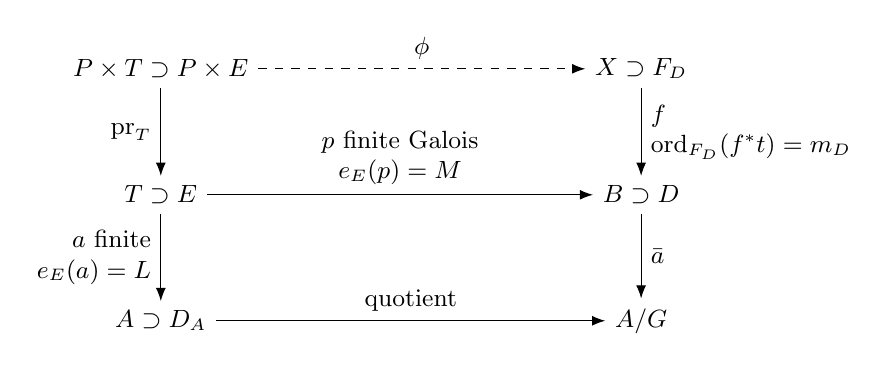
\begin{tikzpicture}[>=Latex, every node/.style={font=\small}]
 \node (prod) at (0,1.6) {\(P\times T\supset P\times E\)};
 \node (source) at (6.1,1.6) {\(X\supset F_D\)};
 \node (cover) at (0,0) {\(T\supset E\)};
 \node (base) at (6.1,0) {\(B\supset D\)};
 \node (abelian) at (0,-1.6) {\(A\supset D_A\)};
 \node (quotient) at (6.1,-1.6) {\(A/G\)};
 \draw[->,dashed] (prod) -- node[above] {\(\phi\)} (source);
 \draw[->] (prod) -- node[left] {\(\operatorname{pr}_T\)} (cover);
 \draw[->] (source) -- node[right,align=left]
   {\(f\)\\\(\operatorname{ord}_{F_D}(f^*t)=m_D\)} (base);
 \draw[->] (cover) -- node[above,align=center]
   {\(p\) finite Galois\\\(e_E(p)=M\)} (base);
 \draw[->] (cover) -- node[left,align=right]
   {\(a\) finite\\\(e_E(a)=L\)} (abelian);
 \draw[->] (base) -- node[right] {\(\bar a\)} (quotient);
 \draw[->] (abelian) -- node[above] {quotient} (quotient);
\end{tikzpicture}
\end{center}
Here \(t\) is a local uniformizer of \(D\), and \(\phi\) is induced by
the birational identification over \(T\).  The integers \(M\) and
\(L\) are local indices along \(E\), not the degrees of the finite
maps.  They compare to the multiplicity \(m_D\) on the original
source \(X\), which may be greater than one.

All assertions concern generic points of divisors.  We may therefore
discard smaller subsets, split the unramified tangential extension,
and work with smooth transverse polydiscs.  Choose a transverse
parameter \(z\) for \(E\), absorbing a unit so that \(p^*t=z^M\).
Cyclic inertia fixes \(E\) pointwise.  Since \(a\) is finite and
equivariant, it fixes the divisor \(D_A\) pointwise.
A finite affine automorphism with a fixed point is conjugate by a
translation to its linear part; fixing a divisor makes its linear
part either the identity or a pseudoreflection.
The perfect cross pairing gives the same assertion on \(P\).

Let \(\omega=\sigma^n/n!\), with an irrelevant nonzero scalar absorbed
into the choice of a translation-invariant volume form on \(P\).
In the top exterior power of \eqref{iso:cross-term}, every term must
contain all \(n\) \(P\)-directions.  Thus the term \(\beta\) makes no
contribution, and on the smooth product model
\[
             \phi^*\omega=\operatorname{vol}_P\wedge a^*
                                      \operatorname{vol}_A.
\]
Its order along \(P\times E\) is \(L-1\).  More precisely, near the
generic point of \(E\), it is \(u z^{L-1}\operatorname{vol}_{\mathrm{prod}}\),
where
\(\operatorname{vol}_{\mathrm{prod}}
=\operatorname{vol}_P\wedge\operatorname{vol}_T\)
for a nowhere vanishing local top form \(\operatorname{vol}_T\) on \(T\),
and \(u\) is pulled back from a unit at the generic point of \(E\).

Let \(v=\operatorname{ord}_{F_D}\) be the normalized valuation of
the divisor in Lemma~\ref{iso:vertical-divisor}.  The product field is
the compositum \(\C(P\times T)=\C(X)\C(T)\).  Geometric integrality
of the generic fiber makes this a Galois extension of \(\C(X)\) with
group \(G\).  Extend \(v\) to a
normalized divisorial valuation \(w\) of the product field
\(\C(P\times T)\), choosing the extension above \(E\).  Indeed,
conjugating any extension by \(G\) preserves its restriction \(v\)
and moves its base center through all divisors of \(T\) over \(D\).
Write \(r\) for the ramification index of \(w/v\).  Since
\(v(t)=m_D\),
\begin{equation}\label{iso:valuation-multiplicity}
                         r m_D=Mw(z).
\end{equation}
The center of \(w\) on the proper product projects dominantly to \(E\).
In particular the product is smooth at the generic point of this
center, and the unit \(u\) above is a \(w\)-unit.
Denote its log discrepancy by \(A_{\mathrm{prod}}(w)\).
The volume form on the smooth \(X\) has order zero at \(v\).
The order of the same pulled-back top form can therefore be computed
in the finite extension of valuation rings and on the product model:
\begin{equation}\label{iso:top-form-valuation}
 \begin{aligned}
 \operatorname{ord}_w(\phi^*\omega)
   &=r\,\operatorname{ord}_v(\omega)+(r-1)=r-1\\
   &=(L-1)w(z)+A_{\mathrm{prod}}(w)-1.
 \end{aligned}
\end{equation}
The first line uses the different exponent \(r-1\) of a tame
extension of discrete valuation rings; the residue extension is
separable in characteristic zero.  The second line uses
\(\operatorname{ord}_w(\operatorname{vol}_{\mathrm{prod}})
=A_{\mathrm{prod}}(w)-1\).
On the smooth product, the pair defined by the smooth divisor
\(z=0\) is log canonical, so \(A_{\mathrm{prod}}(w)\ge w(z)\).
Consequently \eqref{iso:top-form-valuation} gives
\begin{equation}\label{iso:valuation-discrepancy}
 r=(L-1)w(z)+A_{\mathrm{prod}}(w)
                       \ \ge\ Lw(z).
\end{equation}
This last inequality can also be read in local coordinates:
the pullback of a form containing \(dz\) has order at least
\(w(z)-1\).
Combining \eqref{iso:valuation-multiplicity} and
\eqref{iso:valuation-discrepancy} proves
\eqref{iso:multiplicity-bound}.

Let \(k\) be the inertia order of \(T\to T_l\) along this divisor.
Its image on \(A\) is a group of translations fixing \(a(z=0)\),
so that image is trivial.  Quotienting \(A\) by the translation
group is an isogeny and is everywhere unramified.  The indices in
the two compositions consequently give
\[
                          M=kM_l,\qquad L=kL_l.
\]
In particular \(L_lm_D\le M_l\), which implies
\eqref{iso:linear-ramification-bound}.
\end{proof}

\begin{lemma}\label{iso:order-two}
Let \(g_D\) be a local inertia generator at a prime base divisor \(D\).
The linear part of \(g_D^{m_D}\) on \(P\) does not have order two.
\end{lemma}

\begin{proof}
Set \(m=m_D\), and make the base change \(t=s^m\).
Near the generic point of \(D\), the normalized source \(X'\) of this
base change is smooth and its map to \(X\) is \'{e}tale.
Indeed \(f^*t\) has the single divisor \(mF_D\).
In the regular local rings of \(X\) one can write
\(f^*t=u h^m\), with \(u\) a unit; adjoining \(s\) and normalizing
adjoins an \(m\)-th root of the unit.  This is \'{e}tale.
Equivalently, the extension is unramified in codimension one and
purity applies.  The divisor \(s=0\) on \(X'\) is reduced.
These statements hold on a neighborhood of the whole fiber over
the generic point of \(D\), which is the neighborhood used below.

Put \(\delta=\gcd(M,m)\).
On a component of the normalized compositum of the two base covers,
use a parameter \(z'\) so that
\[
 z=(z')^{m/\delta},\qquad
 s=(z')^{M/\delta}.
\]
Its cyclic inertia over the rooted base has order
\[
             M'=\frac M\delta,
 \qquad\text{and its generator acts on \(P\) as }g_D^m.
\]
The order of the pulled-back volume on the new product is \(L'-1\),
where
\begin{equation}\label{iso:rooted-indices}
                         L'=\frac{Lm}{\delta}.
\end{equation}
This follows by substituting \(z=(z')^{m/\delta}\) in
\(z^{L-1}dz\).  In particular
\(0<L'\le M'\), by \eqref{iso:multiplicity-bound}.

Write \(T'\) for the chosen normalized cover, \(E'\) for its divisor
\(z'=0\), and \(\phi':P\times T'\dashrightarrow X'\) for the induced
rational map.  Let \(\omega'\) be the pullback of \(\omega\) to \(X'\);
it is nowhere vanishing on the smooth neighborhood just described.
We first show that the full affine inertia action has a common fixed
point.  Take an actual divisor of \(X'\) over \(s=0\), with normalized
valuation \(v'\), and extend it to a normalized divisorial valuation
\(w'\) of the product field above \(E'\).
Geometric integrality of the generic fiber makes this field extension
Galois with the same group as \(T'\) over the rooted base.
Let \(r'=e(w'/v')\); in this tame Galois extension it is also the
inertia order.  Since \(v'(s)=1\), reducedness gives
\[
                     r'=M'w'(z').
\]
The center \(Z\) of \(w'\) on the proper product projects dominantly
to \(E'\).  Thus
\[
             \kappa(E')\ \subset\ \kappa(Z)\ \subset\ \kappa(w').
\]
Every inertia element fixes \(\kappa(w')\); its restriction to the
base therefore fixes \(\kappa(E')\) and belongs to the cyclic base
inertia of order \(M'\).
Hence \(r'\le M'\), and therefore
\[
                         r'=M',\qquad w'(z')=1.
\]
Thus the whole cyclic base inertia fixes \(\kappa(w')\), and hence
\(\kappa(Z)\).  The generic point of \(Z\) supplies a point of \(P\)
over \(\kappa(Z)\) fixed by this full affine group.  Its common fixed
locus is a constant closed subscheme of \(P\), so nonemptiness after
that field extension implies nonemptiness over \(\C\).
Translation by a complex fixed point conjugates the affine action to
the linear action.  In particular their orders agree.

Suppose now that the linear action has order two.
It is a pseudoreflection, so its determinant on the top fiber form
is \(-1\).  A generator rotates \(z'\) by a primitive \(M'\)-th
root \(\zeta\).
The leading coefficient of the volume is independent of the
\(P\)-variable, and inertia fixes the tangential base residue field.
Invariance of the volume therefore gives
\[
                          -\zeta^{L'}=1.
\]
Thus \(M'\) is even and \(L'\equiv M'/2\pmod {M'}\).
The bound \(0<L'\le M'\) makes this
\[
                              L'=M'/2.
\]

Consider instead the product divisor \(P\times E'\) itself, with its
normalized valuation \(w_0\).
The cyclic base inertia acts on \(\kappa(w_0)\) through its affine
action on \(P\), of order two.  If \(v_0\) is the normalized restriction
to the field of \(X'\), every element of the inertia of \(w_0/v_0\)
fixes \(\kappa(E')\) and therefore lies in this base inertia.
It is exactly the kernel of the displayed residue action, so
\[
                         e_0=e(w_0/v_0)=M'/2.
\]
Properness over the rooted base supplies a center for \(v_0\) on
\(X'\).  It lies in the smooth neighborhood of the whole fiber over
the generic point of \(s=0\).  Thus, even before knowing whether
\(v_0\) is a divisor on \(X'\), the nowhere vanishing form
\(\omega'\) satisfies
\(\operatorname{ord}_{v_0}(\omega')=A_{X'}(v_0)-1\).
Computing the top-form order and the order of \(s\) in the finite
extension gives
\[
 \begin{aligned}
 L'-1
   &=e_0\operatorname{ord}_{v_0}(\omega')+(e_0-1)
     =e_0A_{X'}(v_0)-1,\\
 M'&=w_0(s)=e_0v_0(s).
 \end{aligned}
\]
Since \(L'=e_0=M'/2\), these equalities say
\[
                  A_{X'}(v_0)=1,\qquad v_0(s)=2.
\]
A normalized divisorial valuation over a smooth variety
with log discrepancy one is the valuation of a divisor on that
variety: a center of codimension at least two has log discrepancy
at least two, as is seen by taking regular parameters at its
generic point.  Hence \(v_0\) is an actual divisor of the smooth
source \(X'\).
Its displayed multiplicity two contradicts the reduced divisor
defined by \(s\).  This proves the lemma.
\end{proof}

The two local conclusions have separate uses.  The inequality
\(L_l\le M_l\) will make pulled-back differentials regular near the
minimal stratum.  The order bound for \(g_D^{m_D}\), together with
normal generation by powered meridians, now bounds the dimension.

\begin{lemma}\label{iso:dimension-bound}
The linear monodromy \(G_l\) acts irreducibly on
\(\operatorname{Lie}(P)\), is generated by pseudoreflections of order
greater than two, and satisfies \(n\le4\).
\end{lemma}

\begin{proof}
Choose a connected dense open \(B^\circ\) on which \(f\) is smooth,
the base cover is unramified, and the product description in
Lemma~\ref{iso:abelian-model} holds.  Write \(X^\circ=f^{-1}(B^\circ)\).
The smooth proper map \(X^\circ\to B^\circ\) has connected fibers,
so its map of fundamental groups is surjective.
Since \(X\) is simply connected,
\(\pi_1(X^\circ)\) is normally generated by small meridians around
the divisorial boundary of \(X^\circ\).  One obtains this statement
by filling loops and putting the filling discs in general position;
the subset of complex codimension at least two does not contribute.
Equidimensionality ensures that the inverse image of a subset of
base codimension at least two also has codimension at least two.
By Lemma~\ref{iso:vertical-divisor}, a meridian around \(F_D\)
projects to the \(m_D\)-th power of a meridian around \(D\).

The unramified restriction of \(T\to B\) is connected, and hence its
monodromy has full image \(G\).
Translation parts act trivially on \(H^1(P)\); the linear monodromy
is therefore exactly \(G_l\).
The preceding normal generation says that it is generated by
conjugates of the linear parts of \(g_D^{m_D}\).
Lemma~\ref{iso:ramification} makes each nontrivial such part a
pseudoreflection; Lemma~\ref{iso:order-two} excludes order two.
Notice that generation uses the powered meridians.  Replacing
them by unpowered inertia would lose this conclusion.

The global invariant cycle theorem, applied to the smooth projective
family \(X^\circ\to B^\circ\) and its smooth projective compactification
\(X\), identifies
\[
       H^2(P,\C)^{G_l}
       =\operatorname{im}\bigl(H^2(X,\C)\longrightarrow H^2(P,\C)\bigr).
\]
The hypotheses here are the algebraic smooth family over the connected
open and the proper smooth compactification; no assertion about
invariants on an arbitrary analytic disc is being used
\cite[Th\'eor\`eme~4.1.1(ii)]{Deligne1971}.
The classes \(e,[\sigma],[\overline\sigma]\) restrict to zero,
and the ample class restricts nontrivially.
These four classes span \(H^2(X,\C)\), so the displayed space has
dimension one.

If \(\operatorname{Lie}(P)\) had a nontrivial invariant splitting,
average a positive Hermitian form over the finite group and take an
orthogonal invariant splitting.  The imaginary parts of its
restrictions to the two summands give two independent invariant
real alternating forms on the underlying real tangent space.
Their constant forms represent independent classes in
\(H^2(P,\C)^{G_l}\), a contradiction.  Thus the representation is
irreducible.

We use the following precise consequence of the reflection
classification.  An irreducible finite complex reflection group
generated by reflections of order greater than two has dimension
at most four.  Indeed, in the imprimitive case the imprimitivity
spaces are lines and every reflection is either diagonal or has
a two-coordinate block
\[
                       \begin{pmatrix}0&u\\u^{-1}&0\end{pmatrix}.
\]
The latter has order two; diagonal reflections alone cannot generate
an irreducible representation of dimension greater than one.
These are exactly the alternatives in
\cite[\S2, pp.~276--277]{ShephardTodd1954}.
In the primitive case,
\cite[Proposition~(5.9)(iii), p.~430]{Cohen1976}
states that dimension at least five permits no reflection of
order greater than two.  Applying this consequence proves \(n\le4\).
\end{proof}

Suppose, towards a contradiction, that a nonquotient germ remains.
Take \(S_0,\cS,d,c\) from Proposition~\ref{str:minimum}.
The transverse klt germ on a maximal chart has dimension \(c\).
It cannot have dimension one, since a normal curve is smooth.
It cannot have dimension two, since a klt surface germ is a quotient
germ and its maximal quasi-\'etale cover is smooth
\cite[Proposition~(6.11)]{ClemensKollarMori1988}.
Thus \(c\ge3\).
Proposition~\ref{eu:euler-zero} excludes \(d=0\).
Lemma~\ref{iso:dimension-bound} now forces
\begin{equation}\label{iso:elliptic-case}
              n=4,\qquad c=3,\qquad d=1,\qquad
              \chi_{\mathrm{top}}(S_0)=0.
\end{equation}
The coarse curve \(S_0\) is normal and projective, hence smooth.
Its Euler number makes it a curve of genus one.
The remainder of the proof rules out this last possibility.

\begin{lemma}\label{iso:local-fields}
For \(z_0\in T_l\), put \(J=\operatorname{Stab}_{G_l}(z_0)\) and
\[
                V_J=\operatorname{Lie}(A_l)^J.
\]
Every translation field belonging to \(V_J\) lifts to a holomorphic
vector field on a neighborhood of \(z_0\) in \(T_l\).  This lift is
\(J\)-invariant and descends through \(p_l\).
If \(p_l(z_0)\in S_0\), then \(\dim V_J\le1\).
\end{lemma}

\begin{proof}
First describe the branch divisors of \(a_l\).
If \(R\subset T_l\) has ramification index \(L_l>1\), then
\eqref{iso:linear-ramification-bound} implies \(M_l>1\) for \(p_l\).
Its nontrivial cyclic inertia fixes \(R\) pointwise and therefore
fixes the divisor \(a_l(R)\) pointwise.
Since the linear action of \(G_l\) is faithful, a generator acts
on \(A_l\) by an affine pseudoreflection.
Consequently \(a_l(R)\) is a component of its fixed locus:
it is a translate of an abelian subvariety of codimension one.
We call such a translate an abelian hyperplane.

After shrinking about \(z_0\), every ramification divisor that meets
the neighborhood contains \(z_0\).
Its inertia is contained in \(J\), since an automorphism fixing
the divisor pointwise fixes \(z_0\).
The tangent hyperplane of its image therefore contains \(V_J\).

Let \(v\in V_J\).
The finite separable map \(a_l\) gives a unique meromorphic lift
\(\widetilde v\) of the constant field \(v\).
It is regular in codimension one.
At an unramified generic point this is immediate.
At a general point of a ramification divisor choose coordinates
in which \(a_l\) is
\[
        (z,y_2,\ldots,y_n)\longmapsto
                     (z^{L_l},y_2,\ldots,y_n).
\]
Since \(v\) is tangent to the abelian branch hyperplane, its normal
component is zero and the lift has no pole.
Normality then extends the derivation everywhere: for any regular
function \(h\), the meromorphic function \(\widetilde v(h)\)
belongs to every local height-one ring and thus to the normal
local ring itself.
Uniqueness of the lift and \(J\)-invariance of \(v\) show that
\(\widetilde v\) is \(J\)-invariant.
The germ of \(p_l\) is the quotient by \(J\), so the field descends
to that germ of \(B\).

These descended fields have independent evaluations.
To verify this without assuming either germ smooth, center
exponential coordinates of \(A_l\) at \(a_l(z_0)\), so the finite
affine \(J\)-action becomes linear.
Choose \(J\)-invariant linear coordinate functions
\(\ell_1,\ldots,\ell_r\), dual to a basis
\(v_1,\ldots,v_r\) of \(V_J\).
The invariant functions \(a_l^*\ell_i\) descend to functions
\(u_i\) on the base germ, and the descended fields \(\xi_j\) satisfy
\[
                              \xi_j(u_i)=\delta_{ij}.
\]
They therefore split \(r\) smooth directions by their local flows.
The same directions persist on the maximal quasi-\'etale chart:
the fields lift uniquely across a quasi-\'etale finite map
(check regularity in codimension one and use normality), and
the pulled-back functions retain these identities.
On \(S_0\) the evaluation rank on that chart is \(d=1\), by
Proposition~\ref{str:minimum}.  Thus \(r\le1\).
\end{proof}

\begin{lemma}\label{iso:regular-differentials}
For every local holomorphic function \(u\) on \(B\), its pulled-back
differential has an expression
\begin{equation}\label{iso:differential-coefficients}
                 p_l^*(du)=\sum_{i=1}^n h_i\,a_l^*\alpha_i,
\end{equation}
where the \(\alpha_i\) are a basis of translation-invariant
one-forms on \(A_l\) and the \(h_i\) are holomorphic on the
corresponding neighborhood of \(T_l\).
At a point \(z_0\) with stabilizer \(J\), the covector
\(\sum_i h_i(z_0)\alpha_i\) is \(J\)-invariant.
\end{lemma}

\begin{proof}
The coefficients are uniquely defined meromorphic functions, since
\(a_l\) is generically \'{e}tale.
It is enough to check regularity at every prime divisor of \(T_l\).
There is nothing to prove where \(a_l\) is unramified.
At a general ramification point write \(M=M_l\), \(L=L_l\).
Use linear coordinates \((x,y_2,\ldots,y_n)\) on \(A_l\) adapted
to the affine fixed hyperplane \(x=0\).
The inertia fixes the \(y_i\) and acts on \(x\) by a root of unity.
The restrictions of \(a_l^*y_i\) are generically independent along
the divisor.  They can be used as tangential coordinates on
\(T_l\), and, after absorbing a unit in the normal parameter,
\[
                       a_l^*x=z^L.
\]
Choose \(z\) so that the cyclic inertia rotates it by a primitive
\(M\)-th root.  The local invariant ring of this cyclic quotient
has coordinates \(z^M,y_2,\ldots,y_n\).
Thus \(p_l^*u=F(z^M,y)\) for a holomorphic function \(F\), and
\[
 d(p_l^*u)
   =\frac ML z^{M-L}F_t(z^M,y)\,d(z^L)
       +\sum_{i=2}^n F_{y_i}(z^M,y)\,dy_i.
\]
All coefficients are holomorphic because \(L\le M\).
The displayed coordinate covectors are constant linear combinations
of the \(\alpha_i\), so this proves the required codimension-one
regularity.  Normality extends every \(h_i\).

Expression \eqref{iso:differential-coefficients} is unique on the
function field.  Its left side is \(J\)-invariant and its right
side transforms by the linear representation on the \(\alpha_i\).
Evaluation at the \(J\)-fixed point \(z_0\) therefore gives an
invariant covector, as asserted.
\end{proof}

\begin{lemma}\label{iso:elliptic-lift}
Let \(C\) be an irreducible component of
\((p_l^{-1}(S_0))_{\mathrm{red}}\).
Then \(C\) is a smooth curve of genus one.
Its image \(E=a_l(C)\) is an elliptic translate in \(A_l\), and
\(a_l|_C:C\to E\) and \(p_l|_C:C\to S_0\) are \'{e}tale.
At every \(z\in C\),
\[
       \operatorname{Lie}(A_l)^{\operatorname{Stab}_{G_l}(z)}
                            =\operatorname{Lie}(E).
\]
Here \(\operatorname{Lie}(E)\) means the constant tangent direction
of the translate \(E\).
\end{lemma}

\begin{proof}
All components \(C\) are projective curves mapping finitely onto
\(S_0\).  Let \(J_0\) be their generic pointwise stabilizer.
More explicitly, discard the proper fixed loci of those finitely
many group elements that do not fix \(C\) identically.
On the remaining open the stabilizer is the subgroup \(J_0\)
fixing \(C\) pointwise.
Equivariance implies
\[
                         a_l(C)\subset A_l^{J_0}.
\]
Every component of this fixed locus is a translate of an abelian
subvariety with tangent space \(V_{J_0}\).
Lemma~\ref{iso:local-fields} bounds its dimension by one, whereas
finiteness of \(a_l\) makes the image of \(C\) one-dimensional.
It follows that the image is exactly an elliptic translate \(E\),
and \(V_{J_0}=\operatorname{Lie}(E)\).

Write \(\nu:\widehat C\to C\) for the normalization and let
\[
           b:\widehat C\to S_0,\qquad
           a_C:\widehat C\to E
\]
be the two finite morphisms.
At any \(q\in\widehat C\), choose a parameter \(u\) on the smooth
curve \(S_0\) near \(b(q)\), and extend it to a local function on
\(B\).  Such an extension exists because \(S_0\) has its reduced
closed-subspace structure.
Restricting \eqref{iso:differential-coefficients} gives
\begin{equation}\label{iso:curve-differential}
                          b^*du=\eta\,a_C^*\theta
\end{equation}
near \(q\), where \(\theta\) is a nonzero translation-invariant
one-form on \(E\) and \(\eta\) is holomorphic.
There is no assumption here that \(T_l\) is smooth along \(C\).
To justify restriction, first pull
\eqref{iso:differential-coefficients} to a resolution of \(T_l\).
Both sides are regular ordinary differentials there and agree
generically, hence everywhere.  A component of the proper base
change dominating \(\widehat C\) then gives the stated equality
on \(\widehat C\), since pullback of differentials along a dominant
map to a smooth curve in characteristic zero is injective.

Equation \eqref{iso:curve-differential} implies pointwise
\[
                       \operatorname{ram}_q(b)
                          \ge\operatorname{ram}_q(a_C).
\]
Both targets have genus one.  Riemann--Hurwitz therefore gives
the same total ramification degree, \(2g(\widehat C)-2\), for
both maps.  The pointwise inequalities must all be equalities.
In particular \(\eta(q)\ne0\).

Put \(z=\nu(q)\) and \(J=\operatorname{Stab}_{G_l}(z)\).
The covector in Lemma~\ref{iso:regular-differentials} is
\(J\)-invariant, and the nonvanishing of \(\eta(q)\) says that
its restriction to \(\operatorname{Lie}(E)\) is nonzero.
Since \(J\) contains \(J_0\), we have
\[
                         V_J\subset V_{J_0}
                                      =\operatorname{Lie}(E).
\]
A finite-dimensional representation of a finite group in
characteristic zero has equally dimensional invariant vector
and covector spaces, by the averaging projector.
Thus \(V_J\ne0\), and the displayed inclusion is equality.
This holds at every point and on every normalization branch.

Fix a nonzero \(v_0\in\operatorname{Lie}(E)\).
Its unique meromorphic lift through \(a_l\) is holomorphic near
each point of \(C\), by Lemma~\ref{iso:local-fields}, and the
lifts agree on overlaps by uniqueness.
Call the resulting field \(\widetilde v_0\).
It has nonzero evaluation everywhere on \(C\), since
\(da_l(\widetilde v_0)=v_0\).
Locally it descends through \(p_l\) to a field on \(B\).
Its flow preserves the intrinsically defined minimum stratum
\(S_0\), and hence its lifted flow preserves the reduced inverse
image and each of its irreducible curve components.
Thus \(\widetilde v_0\) is tangent to \(C\).

A reduced curve carrying such a nonvanishing ambient holomorphic
field is smooth: choose a function whose derivative under the
field is nonzero, and use the local flow to split off its disc
direction.  An invariant reduced curve in this product is the
disc times a reduced zero-dimensional germ.
It follows that \(C=\widehat C\) is smooth.
Since \(da_l(\widetilde v_0)=v_0\ne0\), the map \(C\to E\) is
unramified.  It is consequently an \'{e}tale cover of an elliptic
curve, so \(g(C)=1\).
The equality of ramification divisors already proved also makes
\(C\to S_0\) unramified.
\end{proof}

\begin{proof}[Proof of Proposition~\ref{iso:exclusion}]
If a nonquotient germ remained, \eqref{iso:elliptic-case} and
Lemma~\ref{iso:elliptic-lift} would supply \(C\) and a nonzero
translation direction \(v_0\) as above.
Choose a positive integer \(r\) such that
\(\mathcal L=\cO_B(rK_B)\) is a line bundle, and put
\[
                         \mathcal M=p_l^*\mathcal L.
\]
We construct a holomorphic connection on \(\mathcal M|_C\);
in particular we must check both its extension and its gluing.

Near \(z\in C\), the field \(\widetilde v_0\) is invariant under
the point stabilizer and descends to a holomorphic field
\(\xi_z\) on the corresponding base germ.
On \(B_{\mathrm{reg}}\), Lie differentiation by \(\xi_z\) acts
on \(r\)-fold canonical tensors.  It extends to an operator
\[
             \mathcal D_z:\mathcal L\longrightarrow\mathcal L.
\]
Indeed \(\mathcal L\) is the reflexive extension of its restriction
to \(B_{\mathrm{reg}}\), so a differentiated section extends
uniquely across the subset of codimension at least two.
The operator obeys
\[
             \mathcal D_z(us)
                    =\xi_z(u)s+u\mathcal D_z(s).
\]
Pull it to the chosen neighborhood in \(T_l\) using the lifted
symbol \(\widetilde v_0\): in a local pulled-back frame its rule is
\begin{equation}\label{iso:connection-operator}
 \widetilde{\mathcal D}_z(h\,p_l^*s)
       =\widetilde v_0(h)\,p_l^*s
                   +h\,p_l^*(\mathcal D_zs).
\end{equation}
The Leibniz identity and
\(\widetilde v_0(p_l^*u)=p_l^*(\xi_z u)\)
make this definition independent of the frame.

On an overlap, both operators
\(\widetilde{\mathcal D}_z\) have the same symbol.
They agree on the dense open where \(p_l\) is \'{e}tale and
both varieties are smooth: there the differential of \(p_l\)
identifies the pulled-back canonical tensors with canonical
tensors upstairs, and both operators are Lie differentiation
by the same field \(\widetilde v_0\).
Their difference is an \(\cO_{T_l}\)-linear endomorphism of the
line bundle \(\mathcal M\); its coefficient is holomorphic and
zero on a dense open, hence is zero.
Thus the local operators glue on a neighborhood of \(C\).
This argument compares the operators upstairs and does not
require a single descended vector field on a neighborhood of
all of \(S_0\).

Tangency of \(\widetilde v_0\) to the reduced curve \(C\) implies
that the glued operator preserves
\(\mathcal I_C\mathcal M\), by
\eqref{iso:connection-operator}.
It therefore induces a first-order operator
\[
             D:\mathcal M|_C\longrightarrow\mathcal M|_C
\]
with symbol the nowhere vanishing field
\(\widetilde v_0|_C\).
Let \(\tau\) be the holomorphic one-form on the elliptic curve
\(C\) satisfying \(\tau(\widetilde v_0)=1\).
Then
\[
                           \nabla s=D(s)\otimes\tau
\]
is a holomorphic connection on \(\mathcal M|_C\).

A line bundle with a holomorphic connection on a smooth projective
curve has degree zero, a classical connection obstruction
\cite{Atiyah1957}.  One elementary proof takes a nonzero
meromorphic section \(s\): the meromorphic one-form
\(\nabla s/s\) has at each point the residue
\(\operatorname{ord}_q(s)\), and the residue theorem gives
\(\deg\operatorname{div}(s)=0\).
Consequently
\[
                         \deg(\mathcal M|_C)=0.
\]
On the other hand, \(-K_B\) is ample as a \(\Q\)-Cartier divisor,
and \(p_l|_C\) is finite onto the positive-dimensional curve
\(S_0\).  Hence
\[
             \deg(\mathcal M|_C)
               =r\,\deg\bigl((p_l|_C)^*K_B\bigr)<0.
\]
This contradiction excludes the nonquotient germ and proves
Proposition~\ref{iso:exclusion}.
\end{proof}

\section{A second Lagrangian system}
\label{secsys:section}
\label{sec:second-system}

Retain the local $e$-locus $D$ and its cohomology marking from
Proposition~\ref{def:fixed-base}, and write $f_0:X_0\to B$ for the
original projective fibration.  The geometric target is an actual nearby
manifold with two integral nef isotropic classes whose entire positive
interval lies in its K\"ahler cone.  This gives both fibrations on one
projective manifold, with the first still mapping to the original $B$.

\begin{proposition}[Two systems on one nearby model]\label{secsys:second-system}
Arbitrarily close to the original point of $D$, there is a member
$X'=X_t$ and an integral $(1,1)$-class $u$ such that $e$ and $u$ are
nef and
\[
                  q(e)=q(u)=0,\qquad q(e,u)>0,
\]
and the whole positive interval satisfies
\begin{equation}\label{secsys:geometric-target}
             \{a e+b u:a,b>0\}\subset\mathcal K_{X'}.
\end{equation}
In particular $X'$ is projective.  Its fixed-base fibration
$f'=f_t:X'\to B$ admits a second projective Lagrangian fibration
$g:X'\to C$, with $C$ normal and projective.  For every fiber $A$
over the smooth locus of $g$, the restriction $f'|_A:A\to B$ is
finite and surjective.  Thus $B$ has a finite cover by an abelian variety.
\end{proposition}

The rank-four refinement proved in
Proposition~\ref{secsys:rank-four-variation} chooses $g$ with nonzero
polarized variation when the original fibration has that property.
We first construct the two classes in
\eqref{secsys:geometric-target}.

We distinguish integral isometries from parallel-transport operators
throughout the proof.  This distinction matters in applying Torelli.
Write $\Lambda=H^2(X_0,\Z)$, equipped with $q$, and fix the connected
marked deformation component containing $X_0$.  Its orientation of maximal
positive subspaces is the one given by
$(\operatorname{Re}\sigma_0,\operatorname{Im}\sigma_0,\kappa)$, with
$\kappa$ K\"ahler.  Markings below are anchored by parallel transport
in this component.

\subsection{Realized positive three-planes}

Call an oriented positive three-plane $T\subset\Lambda_{\R}$
\emph{realized} if it is the span of the period plane and a K\"ahler
class of a marked manifold in the chosen component.  The Calabi--Yau
theorem and twistor rotation imply that every compatible oriented
two-plane $P\subset T$, together with its positively oriented orthogonal
ray in $T$, is realized once $T$ is realized.  We use period surjectivity
from the chosen marked component for the integral Beauville lattice
\cite[\S3.1 and Theorem~5.5]{HuybrechtsTorelli2012}, together with the
marked period identification
\cite[Corollaries~4.10 and~5.9]{HuybrechtsTorelli2012}.
The K\"ahler form of parallel-transport Torelli says that a Hodge
parallel-transport isometry carrying a K\"ahler class to a K\"ahler
class is induced by an isomorphism
\cite[Theorem~1.3(2) and \S3.2]{Markman2011}.  The global Torelli input
in that proof is the preceding marked period identification.
These are the marked-component statements used below.
The twistor description is also recalled in
\cite[Section~5.1]{AmerikVerbitsky2015}.

\begin{lemma}\label{secsys:metric-periods}
Realized positive three-planes form an open subset.  In rank greater
than four, a three-plane fails to be realized precisely when it is
orthogonal to a rational negative MBM class of the marked component.
In rank four, the weaker assertion that every nonrealized three-plane
has a rational negative orthogonal line suffices and holds.
At a fixed oriented period, K\"ahler cones of marked models in the
component are either equal or disjoint.
\end{lemma}

\begin{proof}
Given a realized pair $(P,\kappa)$, nearby planes $T'$ contain oriented
period planes $P'$ close to $P$ and orthogonal positive vectors
$\kappa'$ close to $\kappa$.  Local Torelli realizes $P'$ by a small
deformation of that manifold.  Openness of the relative K\"ahler cone
makes $\kappa'$ K\"ahler, proving openness.

Recall the two parts of the MBM theorem used here: the negative rational
wall classes are invariant under deformation that keeps them of type
$(1,1)$, and the K\"ahler cone is a component of the positive cone
after removing their orthogonal hyperplanes
\cite[Theorems~1.17 and~1.19]{AmerikVerbitsky2015}.
No bound on their squares is used.  A realized plane cannot be
orthogonal to such a class: that class would be of type $(1,1)$ and
orthogonal to a K\"ahler class.  Conversely, suppose $T$ has no such
orthogonality.  Choose a generic oriented plane $P\subset T$, so that
every rational class orthogonal to $P$ is already orthogonal to $T$.
Indeed, each rational vector not orthogonal to $T$ excludes a proper
closed subset of the sphere of planes in $T$, and there are only
countably many such vectors.  Period surjectivity gives a marked
manifold with period $P$.  Its rational $(1,1)$ classes include no
MBM class.  The cone theorem therefore identifies its K\"ahler cone
with the whole positive component.  The orthogonal ray to $P$ in $T$,
with sign fixed by the orientation, is in that component.  This realizes
$T$.

For rank four one can avoid even the MBM formulation in this step.
If the negative line $T^\perp$ is irrational, the same generic choice
of $P$ has zero Picard lattice.  Its K\"ahler cone is the whole positive
component, so $T$ is realized.  Thus a nonrealized plane has rational
negative normal line.

Finally, an intersection between the K\"ahler cones of two marked models
with the same period gives a Hodge parallel-transport isometry carrying
a K\"ahler class to a K\"ahler class.  Torelli makes it the isometry of
an isomorphism.  The cones then agree.
\end{proof}

Choose an integral ample class $h$ on $X_0$.  A first arbitrarily small
deformation preserving both $h$ and $e$ makes the real period plane
$P_*$ rational: rational positive two-planes are dense in the rational
space $\langle e,h\rangle^\perp$.  In rank four this plane is already
rational, and we take the original point.  Ampleness of $h$ persists, and
Proposition~\ref{def:fixed-base} preserves the fibration of class $e$.
Denote this projective member and its fibration by $X_*,f_*$.
Set
\begin{equation}\label{secsys:four-space}
 U=P_*\oplus\langle e,h\rangle_{\Q},
 \qquad \operatorname{sign}(q|_U)=(3,1).
\end{equation}
Here and below a rational plane is also used for its real span when
discussing signs and periods.  The space
$P_*+\R h$ is realized.  Consequently $U^\perp$ contains no MBM
class that could obstruct realization.

Let $\mathbb H(U)$ be the hyperbolic three-space of negative lines in
$U_{\R}$.  A point $[v]$ corresponds to the positive three-plane
$v^\perp\cap U_{\R}$, with its fixed orientation.  Let
$J\subset\mathbb H(U)$ be the set of nonrealized planes.  It is closed
by Lemma~\ref{secsys:metric-periods}.  Moreover,
\begin{equation}\label{secsys:rational-bad-set}
             J\subset\mathbb H(U)(\Q).
\end{equation}
For rank greater than four, project an obstructing rational MBM class
orthogonally to $U$.  The projection is rational and nonzero, since
$U^\perp$ contains no such class; it is the negative normal line in
$U$.  In rank four use the last assertion about nonrealized planes in
Lemma~\ref{secsys:metric-periods}.  Any parallel-transport isometry
preserving $U$ preserves $J$.

Choose the component of the negative cone whose null boundary contains
the ray $\R_{>0}e$.  We call its nonzero vectors, including boundary
vectors, future vectors.  Distinct future null vectors have negative
pairing.  The other null line in $\langle e,h\rangle$ has a rational
future representative
\begin{equation}\label{secsys:other-cusp}
 w_*=e-\frac{2q(e,h)}{q(h)}h.
\end{equation}
The negative lines in a Lorentz plane with future null boundary vectors
$v,w$ form the geodesic
$\{[s v+t w]:s,t>0\}$; we denote it by $(v,w)$.

\subsection{Null rotations from actual algebraic families}

\begin{lemma}\label{secsys:actual-monodromy}
Let $a\in U_{\Q}$ be nonzero and null.  Every rational null rotation
fixing $a$, extended as the identity on $U^\perp$, has a positive power
that is an integral parallel-transport operator in the chosen marked
component.
\end{lemma}

\begin{proof}
Choose $b\in U_{\Q}$ with $q(a,b)=1$ and $q(b)=0$; subtracting
$q(b_0)a/2$ from any $b_0$ paired to $1$ with $a$ gives such a vector.
Let $V=\langle a,b\rangle^\perp\cap U$, a positive rational plane.
For $x\in V_{\Q}$ the null rotation is
\begin{equation}\label{secsys:null-rotation}
 \begin{split}
 T_{a,x}a&=a,\\
 T_{a,x}b&=b+x-\tfrac12 q(x)a,\\
 T_{a,x}v&=v-q(v,x)a\quad(v\in V),
 \end{split}
 \qquad T_{a,x}|_{U^\perp}=\id.
\end{equation}
Direct pairing verifies that it preserves $q$, and substitution gives
$T_{a,x}T_{a,y}=T_{a,x+y}$.  Thus $T_{a,x}^m=T_{a,mx}$.
Its matrix entries in an integral basis are polynomials in $m$ of degree
at most two with rational coefficients and constant term the identity.
For sufficiently divisible $m$, both $T_{a,mx}$ and its inverse are
integral.  This accounts also for the finite gluing between the
sublattices in $U$ and $U^\perp$.

For $x\ne0$, choose a rational positive vector
$\ell\in V\cap x^\perp$.  The rotation fixes $\ell$.  Replace it by
a primitive integral vector on the same line.  A generic period in
$\ell^\perp$ has Picard lattice $\Z\ell$.  Period surjectivity and
the cone theorem give an ample marked deformation with polarization
$\ell$ or $-\ell$; choose the ample sign.  This sign does not alter
the stabilizer of $\ell$.

We now use the prescribed-polarization conclusion of
\cite[Lemma~4.2]{StrongSYZ2026}.  It applies to this primitive positive
class $\ell$, ample on a manifold in the chosen marked component.
Write $D_\ell$ for the component of its type-IV period domain containing
that ample period, and put
\[
 G_\ell(\Z)=\{g\in O(\Lambda,q):g\ell=\ell,
                                      \ gD_\ell=D_\ell\}.
\]
The cited lemma supplies a smooth projective family of IHS manifolds
over a smooth connected quasi-projective variety $S$, with a relative
polarization of class $k\ell$ for some $k>0$ and a reference marking
obtained by parallel transport from $X_0$.  It also supplies a
torsion-free finite-index subgroup $\Gamma\subset G_\ell(\Z)$
containing the family monodromy and an algebraic period map
\[
           \Phi:S\longrightarrow Q_\ell:=\Gamma\backslash D_\ell.
\]
Here $Q_\ell$ is smooth and quasi-projective, the map
$D_\ell\to Q_\ell$ is a covering with free $\Gamma$-action, and a
local marked lift of $\Phi$ is submersive.  The type-IV domain
$D_\ell$ is contractible, including in rank four, so this covering
identifies $\pi_1(Q_\ell)$ with $\Gamma$.

The remaining finite-index assertion concerns the image of this
actual family monodromy, and we prove it here.  The submersive local
lift makes the algebraic map $\Phi$ dominant.

Choose an irreducible algebraic slice $S'\subset S$ of dimension
$\dim Q_\ell$ dominating $Q_\ell$.  For example, intersect with
general hyperplanes through a smooth submersive point, transverse to
its period fiber.  After normalization and restriction, this slice is
smooth and generically finite over $Q_\ell$.  There is a nonempty
Zariski-open $Q^\circ\subset Q_\ell$ over which its restriction is
a nonempty finite \'{e}tale cover: generic finiteness gives a finite
open after removing the boundary in a proper compactification, and
characteristic zero allows removal of the branch locus.
Therefore its fundamental-group image has finite index in
$\pi_1(Q^\circ)$.  The map
$\pi_1(Q^\circ)\to\pi_1(Q_\ell)$ is surjective, since a loop in a
complex manifold can be moved off a proper algebraic subset.
It follows that
\begin{equation}\label{secsys:finite-index-image}
       [\Gamma:\Phi_*\pi_1(S)]<\infty.
\end{equation}
The period map on the universal cover of $S$, based at this reference
marking, is equivariant for the actual second-cohomology monodromy.
Because $D_\ell\to Q_\ell$ is a
covering with free action, the deck transformation induced by each
loop is exactly that cohomology operator.  Hence the subgroup in
\eqref{secsys:finite-index-image} consists of actual parallel transports,
with the original marking retained.

Our rotation fixes $\ell$; after taking an integral power, a further
power preserves $D_\ell$ and therefore lies in $G_\ell(\Z)$.
Since $\Gamma$ has finite index in $G_\ell(\Z)$, a further power
lies in $\Gamma$; by \eqref{secsys:finite-index-image}, one more
positive power lies in the family monodromy.  This uses only that every element has a
positive power in any finite-index subgroup; normality of the subgroup
is unnecessary.  Transport to the original reference fiber finishes
the proof.  The zero parameter gives the identity.
\end{proof}

\subsection{An integral loxodromic operator with irrational axis}

\begin{lemma}\label{secsys:loxodromic}
There is a parallel-transport operator $\gamma$ preserving $U$ and
acting identically on $U^\perp$ such that its characteristic polynomial
on $U$ is irreducible over $\Q$.  Its real eigenvalues are
$\rho,\rho^{-1}$ with $\rho>1$, and its other two eigenvalues are a
nonreal conjugate pair on the unit circle.  Its attracting and repelling
future null lines $a_+,a_-$ can both be placed in any prescribed
neighborhood of $[w_*]$ in the null boundary.
\end{lemma}

\begin{proof}
Choose a rational null partner $b$ of $e$ on the line of $w_*$ with
$q(e,b)=1$, and a rational orthogonal basis $v_1,v_2$ of their positive
perpendicular plane.  Write $q(v_1)=A>0$, $q(v_2)=B>0$.
For a rational number $t\ne0$, set $x=v_1$, $y=v_1+t v_2$.
Choose $t$ so that
\begin{equation}\label{secsys:phase-choice}
                  \frac{2(A-Bt^2)}{A+Bt^2}\notin\Z.
\end{equation}
This is possible: the expression lies in $(-2,2)$ and assumes each
of the three possible integral values at only finitely many real $t$.
By Lemma~\ref{secsys:actual-monodromy}, for some positive integers
$m_1,m_2$ the opposite rotations $T_{e,m_1x}$ and $T_{b,m_2y}$ are
integral monodromies.

For completeness, the spectral calculation can be performed in a real
orthonormal transverse basis without any rationality assumption on
$\sqrt A$ or $\sqrt B$.  Identify
$a e+b' b+c v_1+d v_2$ with the Hermitian matrix
\[
 \begin{pmatrix}
 \sqrt2 a&\sqrt A c+i\sqrt B d\\
 \sqrt A c-i\sqrt B d&-\sqrt2 b'
 \end{pmatrix}.
\]
Its determinant is the negative of $q$.  The action
$H\mapsto MHM^*$ of $SL_2(\C)$ induces $SO^+(3,1)$.
Formula~\eqref{secsys:null-rotation} corresponds, for the first
rotation, to an upper triangular unipotent with parameter
$-m_1\sqrt A/\sqrt2$; the opposite rotation corresponds to a lower
triangular unipotent with parameter
$m_2(\sqrt A-i t\sqrt B)/\sqrt2$.
Put
\[
            \gamma_k=T_{e,km_1x}T_{b,km_2y}.
\]
Its spin trace is
\begin{equation}\label{secsys:spin-trace}
 \tau_k=2+k^2m_1m_2\zeta,
 \qquad \zeta=-\tfrac12(A-i t\sqrt{AB}).
\end{equation}
Let $\lambda_k,\lambda_k^{-1}$ be its spin eigenvalues, choosing
$|\lambda_k|>1$.  For large $k$,
$\lambda_k/\tau_k\to1$.  The four eigenvalues on $U_{\R}$ are
\[
 |\lambda_k|^2,\quad |\lambda_k|^{-2},\quad
 \lambda_k/\overline{\lambda_k},\quad
 \overline{\lambda_k}/\lambda_k.
\]
The sum of the last pair converges to
$2\cos(2\arg\zeta)=2(A-Bt^2)/(A+Bt^2)$.
By \eqref{secsys:phase-choice}, it is nonintegral for all sufficiently
large $k$.  In particular, this conjugate pair is nonreal and neither
eigenvalue is $1$ or $-1$.

The characteristic polynomial on $U$ is monic with rational
coefficients, and its roots are algebraic integers because
$\gamma_k$ preserves $\Lambda$.  It therefore belongs to $\Z[z]$.
It is reciprocal, has constant term $1$, and has no rational root:
a rational root would be $1$ or $-1$.  If it factored into two
quadratics over $\Q$, real coefficients would force the nonreal pair
to belong to one quadratic.  That monic factor has integral
coefficients, so the sum of the pair would be an integer, a
contradiction.  Thus it is irreducible.  Fix a sufficiently large $k$.

Finally, a nontrivial null rotation fixing $[w_*]$ has powers converging
to $[w_*]$ on every other point of the null boundary.  In boundary
coordinates with $[w_*]$ at infinity these powers are translations
$z\mapsto z+jc$, with $c\ne0$.  Such a rotation has an integral
monodromy power by Lemma~\ref{secsys:actual-monodromy}.  Neither
eigenline of $\gamma_k$ is rational, by irreducibility, so neither is
$[w_*]$.  Conjugating $\gamma_k$ by a sufficiently high power of this
rotation brings both eigenlines as close to $[w_*]$ as desired and
preserves all the asserted properties.  Call the conjugate $\gamma$.
\end{proof}

The axis $(a_-,a_+)$ contains no rational negative line.  Indeed, a
nonzero rational vector in its invariant real Lorentz plane would
have its entire $\gamma$-orbit in that plane.  The rational span of
the orbit would be a nonzero proper rational invariant subspace of
$U$, contradicting irreducibility.  The two geodesics $(e,a_\pm)$
also contain no rational negative line.  Otherwise such a line,
together with rational $e$, would define a rational Lorentz plane.
A rational binary quadratic form with one rational null line has
both null lines rational: if $q(e,v)\ne0$, its second null vector is
$v-q(v)e/(2q(e,v))$.  The second line would be $a_\pm$, contrary
to irreducibility.  Equation~\eqref{secsys:rational-bad-set} gives
\begin{equation}\label{secsys:good-limit-geodesics}
 J\cap(a_-,a_+)=J\cap(e,a_+)=J\cap(e,a_-)=\varnothing.
\end{equation}

\subsection{Uniform tails and the entire K\"ahler interval}

For a future null line $[w]$ near $[w_*]$, choose its representative
with $q(e,w)=-1$ and put
\[
              P(e,w)=\langle e,w\rangle^\perp\cap U_{\R},
\]
oriented near $P_*$.  This is a nearby $e$-period.  It gives an actual
small deformation $X_w$ of $X_*$ within $D$, with the fibration $f_w:X_w\to B$ by
Proposition~\ref{def:fixed-base}.  The orthogonal projection of $h$ to
$\langle e,w\rangle$ has the form
\begin{equation}\label{secsys:projected-kahler}
 h_w=\alpha(w)e-\beta w,\qquad
 \alpha(w)=-q(h,w)>0,\quad \beta=q(h,e)>0.
\end{equation}
It tends to $h$ as $[w]\to[w_*]$, so it is K\"ahler on $X_w$
after restricting to a small neighborhood.  As $e$ is nef on $X_w$,
every $h_w+t e$, $t\ge0$, is K\"ahler.  Its orthogonal negative
line in $\langle e,w\rangle$ is
$[(\alpha(w)+t)e+\beta w]$.  On a smaller neighborhood $\mathcal V$
of $[w_*]$, the continuous function $\alpha(w)/\beta$ is bounded
above by some $R$.  Thus
\begin{equation}\label{secsys:uniform-tail}
 [s e+w]\notin J\qquad
 ([w]\in\mathcal V,\ q(e,w)=-1,\ s\ge R).
\end{equation}
This is the required uniformity near the rational endpoint $e$.
Choose the conjugation in Lemma~\ref{secsys:loxodromic} so that both
$a_+$ and $a_-$ belong to $\mathcal V$.

\begin{lemma}\label{secsys:whole-geodesic}
For all sufficiently large integers $N$,
\[
                         (e,\gamma^N e)\cap J=\varnothing.
\]
\end{lemma}

\begin{proof}
Choose future eigenvectors for $a_+,a_-$ with eigenvalues
$\rho,\rho^{-1}$, respectively.  The remaining real invariant
plane is positive definite and $\gamma$ acts on it by a rotation.
Since $e$ is a future null vector different from both eigenlines,
its coefficients along both future eigenvectors are positive.
Indeed, pairing its eigenspace decomposition with either eigenvector
shows the coefficient of the other to be positive.  It follows that
\begin{equation}\label{secsys:endpoint-limits}
 \rho^{-N}\gamma^Ne\longrightarrow v_+,
 \qquad
 \rho^{-N}\gamma^{-N}e\longrightarrow v_-,
\end{equation}
where $v_+,v_-$ are positive representatives of $a_+,a_-$.

If the assertion failed, choose $N\to\infty$ and
$z_N=[s_Ne+\gamma^Ne]\in J$, with $s_N>0$.  We first claim
\begin{equation}\label{secsys:balance-bounds}
             s_N\rho^{-N}\longrightarrow0,
             \qquad s_N\rho^N\longrightarrow\infty.
\end{equation}
To prove the first limit, normalize $\gamma^Ne$ by
$c_N=-q(e,\gamma^Ne)$; by \eqref{secsys:endpoint-limits},
$c_N/\rho^N$ tends to a positive constant, and
$[\gamma^Ne]\to a_+\in\mathcal V$.
The tail exclusion~\eqref{secsys:uniform-tail} bounds $s_N/c_N$
above.  If a subsequence of $s_N/\rho^N$ had a positive limit,
$z_N$ would converge to an interior point of $(e,a_+)$.
Closedness of $J$ would put that point in $J$, contradicting
\eqref{secsys:good-limit-geodesics}.  This proves the first limit.
Apply the same argument to
\[
 \gamma^{-N}z_N
       =[s_N\gamma^{-N}e+e]
       =[s_N^{-1}e+\gamma^{-N}e]\in J.
\]
The uniform tail at $e$ now uses $a_-\in\mathcal V$ and gives
$s_N^{-1}\rho^{-N}\to0$, which is the second limit.

Choose integers $k_N$ such that
\[
               1\le s_N\rho^{2k_N-N}<\rho^2.
\]
The two limits in \eqref{secsys:balance-bounds} imply
$k_N\to\infty$ and $N-k_N\to\infty$.
Passing to a subsequence, suppose
$s_N\rho^{2k_N-N}\to r\in[1,\rho^2]$.
Apply $\gamma^{-k_N}$ to $z_N$ and divide its representative by
$\rho^{N-k_N}$.  Equation~\eqref{secsys:endpoint-limits} gives
\[
 \frac{s_N\gamma^{-k_N}e+\gamma^{N-k_N}e}{\rho^{N-k_N}}
   =s_N\rho^{2k_N-N}
       \frac{\gamma^{-k_N}e}{\rho^{k_N}}
       +\frac{\gamma^{N-k_N}e}{\rho^{N-k_N}}
   \longrightarrow r v_-+v_+.
\]
The limit has negative square, so its line is an interior point of
the axis $(a_-,a_+)$.  Invariance and closedness of $J$ put that
line in $J$, contradicting \eqref{secsys:good-limit-geodesics}.
\end{proof}

Take such an $N$ and let $X_N$ be the actual nearby $e$-deformation
with first fibration $f_N:X_N\to B$ and period
$P_N=P(e,\gamma^Ne)$, oriented near $P_*$.
The choice of $a_+$ close to $[w_*]$, followed by large $N$, makes
this deformation as small as prescribed.  Put
\begin{equation}\label{secsys:second-class}
 u_N=-\gamma^Ne,\qquad
 \mathcal C_N=\{a e+b u_N:a,b>0\}.
\end{equation}
The minus sign is essential: $e$ and $\gamma^Ne$ are future null
vectors, so $q(e,\gamma^Ne)<0$ and $q(e,u_N)>0$.
The cone $\mathcal C_N$ is a positive component in the Lorentz plane
$\langle e,u_N\rangle$.  Its positive rays correspond, by taking
orthogonal negative lines, to the geodesic $(e,\gamma^Ne)$.
Lemma~\ref{secsys:whole-geodesic} and twistor rotation show that every
ray of $\mathcal C_N$ is K\"ahler on some marked model of period $P_N$.

All those rays are K\"ahler on $X_N$ itself.  Indeed, their projectivized
interval is connected.  Intersections with the K\"ahler cones of marked
models give an open cover by pairwise disjoint sets, by
Lemma~\ref{secsys:metric-periods}.  Such a cover has just one nonempty
member.  The class $h_w$ of \eqref{secsys:projected-kahler}, for
$[w]=[\gamma^Ne]$, belongs to this interval and is K\"ahler on $X_N$.
Thus
\begin{equation}\label{secsys:actual-cone}
                         \mathcal C_N\subset\mathcal K_{X_N}.
\end{equation}
In particular $e+u_N$ is an integral K\"ahler class, making $X_N$
projective, and $u_N$ is a nonzero integral nef isotropic $(1,1)$
class on this very manifold.  It is the Chern class of a line bundle:
the exponential sequence and $H^1(X_N,\cO_{X_N})=0$ identify
$\Pic(X_N)$ with the integral $(1,1)$ classes.  Applying
Theorem~\ref{thm:strong-syz}, including Stein factorization, gives
the second Lagrangian fibration $g:X_N\to C$ with normal projective
base $C$.  Both $f_N$ and $g$ are projective morphisms: their graphs
are closed analytic subvarieties of projective products, hence
algebraic, and the corresponding algebraic maps are projective.

\subsection{Finite maps from its abelian fibers}

Let $A$ be a fiber over the smooth locus of $g$.  It is an abelian
variety after choosing an origin.  A positive multiple of $u_N$ is
$g^*c_1(H_C)$ for an ample line bundle $H_C$ on $C$, so the cohomology
class of $A$ is a positive rational multiple of $u_N^n$.  To see the
constant, cut $C$ by $n$ general hyperplanes in a sufficiently high
multiple of $H_C$; their transverse intersection is a finite collection
of regular points, and its inverse image is the corresponding collection
of fibers.  All regular fibers have the same cohomology class by
parallel transport over the connected smooth locus.

Polarizing Fujiki gives the exact positive quantity
\begin{equation}\label{secsys:mixed-fujiki}
 \binom{2n}{n}\int_{X_N}e^n u_N^n
       =c_{X_N}\,2^n q(e,u_N)^n>0.
\end{equation}
Therefore the nef line bundle $f_N^*H|_A$ has positive top
self-intersection.  Such a line bundle on an abelian variety is ample.
Indeed, average representatives of its class by translations.  Nefness
makes the resulting invariant Hermitian form positive semidefinite,
and positive top intersection makes its determinant positive.  All
its eigenvalues are then positive, so the line bundle has a positive
curvature representative and is ample.

The morphism $f_N|_A$ has no positive-dimensional fiber, since a curve
in such a fiber would have degree zero against this ample line bundle.
It is proper, hence finite.  Its image is closed of dimension
$\dim A=n=\dim B$ and therefore equals $B$.  This proves all assertions
of Proposition~\ref{secsys:second-system}.  In particular we have obtained
\begin{equation}\label{secsys:abelian-cover}
                         p:A\longrightarrow B
\end{equation}
as a finite surjective morphism from an abelian variety.

\subsection{Nonzero variation in rank four}

\begin{proposition}[The rank-four variation refinement]
\label{secsys:rank-four-variation}
If $b_2(X_0)=4$ and the polarized family of smooth fibers of $f_0$
has nonzero variation, the choices in
Proposition~\ref{secsys:second-system} can be made so that $g$ also
has nonzero polarized variation.
\end{proposition}

\begin{proof}
Nonzero variation means that, at some regular fiber, the derivative
in a base direction of its weight-one period map is nonzero.  This
condition persists under small deformations of the fibration: on a
small smooth product neighborhood in the family supplied by
Proposition~\ref{def:fixed-base}, the relative Hodge bundle and that
derivative vary holomorphically, so a chosen nonzero matrix entry
stays nonzero.

The fiber polarization can also be transported.  Its class is the
restriction of an integral ample class on $X_0$.  By
Lemma~\ref{def:restriction-kernel} and topological transport, the
restriction image on a nearby smooth fiber is a rational
one-dimensional space with kernel $e^\perp$.  The restriction of a
K\"ahler class spans its real form, since it pairs positively with $e$,
so the transported integral class
remains of type $(1,1)$.  Positivity on the smooth torus is open.
This gives a polarized family near the chosen fiber, and the same
argument applies at the conjugate fibration.

In rank four the preliminary point was $X_*=X_0$.  Complex
conjugation of its hyperk\"ahler complex structure reverses the
period-plane orientation and the K\"ahler sign.  The resulting marked
manifold $\overline X_*$ has period $\overline P_*$, ample class $-h$,
and conjugate fibration
$\overline f_*:\overline X_*\to\overline B$ with fiber class $-e$.
It lies in the same marked deformation component: a half-circle of
the twistor sphere joins the complex structure to its negative.
Nonzero variation of $\overline f_*$ is equivalent to that of $f_*$.

We choose the endpoint neighborhood in
Lemma~\ref{secsys:loxodromic} small enough for the following comparison
with this conjugate fibration.  Under the actual parallel transport
$\gamma^{-N}$, the underlying plane of $P_N$ becomes
\[
           \langle \gamma^{-N}e,e\rangle^\perp\cap U_{\R}.
\]
It approaches an unoriented plane near $P_*$, since
$[\gamma^{-N}e]\to a_-$ and $a_-$ can be chosen arbitrarily close to
$[w_*]$.  The transported positive cone is
\begin{equation}\label{secsys:opposite-cone}
        \gamma^{-N}\mathcal C_N
             =\{a\gamma^{-N}e-b e:a,b>0\}.
\end{equation}
By \eqref{secsys:other-cusp}, this cone contains a vector close to
$-h$.  Preservation of the orientation of maximal positive
three-spaces therefore makes the transported oriented period close
to $\overline P_*$.

Choose the endpoint neighborhood sufficiently small, and then $N$
sufficiently large, that this period lies in a neighborhood where the
$(-e)$-deformation of $\overline f_*$ exists and has nonzero variation.
Let $Y_N$ be that actual small deformation of $\overline X_*$ with
period $\gamma^{-N}P_N$.  It has a K\"ahler class near $-h$, in the
component \eqref{secsys:opposite-cone}.  In rank four,
$H^{1,1}(X_N,\R)=\langle e,u_N\rangle_{\R}$, so
\eqref{secsys:actual-cone} says that the entire positive component
of $X_N$ is K\"ahler.  The Hodge parallel-transport isometry between
$Y_N$ and $X_N$ induced by $\gamma^N$ consequently carries a
K\"ahler class to a K\"ahler class.  Torelli identifies these
manifolds by an isomorphism inducing that isometry.  The class $-e$
on $Y_N$ becomes $u_N$ on $X_N$.

Line bundles on an IHS manifold are determined by their Chern
classes.  Thus the transported fibration and the fibration obtained
from $u_N$ have the same connected fibers: positive generated powers
define the same Stein factorization.  It follows that $g$ has nonzero
polarized variation.  The isometry in this comparison is the actual
parallel transport constructed in Lemma~\ref{secsys:actual-monodromy}.
\end{proof}

\section{The varying case when \texorpdfstring{$b_2=4$}{b2=4}}
\label{var:section}
\label{sec:variation}

\begin{proposition}[The varying rank-four case]\label{var:exclusion}
Let $X$ be a projective irreducible holomorphic symplectic manifold of
dimension $2n$ with $b_2(X)=4$, and let
\[
                         f:X\longrightarrow B,\qquad
                         g:X\longrightarrow C
\]
be projective Lagrangian fibrations with normal projective bases.
Assume that the polarized family of smooth fibers of $g$ has nonzero
variation and that, for every smooth fiber $A_t$ of $g$, the restriction
$f|_{A_t}:A_t\to B$ is finite and surjective.
Fix a connected minimum stratum $S_0\subset B$ and its smooth
Deligne--Mumford stack $\cS$ as in Propositions~\ref{str:minimum}
and~\ref{str:products}.  Then
\[
 H^{a,b}(\cS)=0\quad\text{for }a\ne b,\qquad
 \chi_{\mathrm{top}}(S_0)=\sum_p h^{p,p}(\cS)>0.
\]
\end{proposition}

Proposition~\ref{secsys:rank-four-variation} supplies these two
fibrations when the original rank-four fibration has nonzero polarized
variation, with the first fibration still mapping to the original
base $B$.  The positive Euler characteristic in the proposition
contradicts Proposition~\ref{eu:euler-zero} when the fixed stratum has
a singular maximal chart.

Fix the data in the proposition, and let $C^\circ$ be the connected
smooth open of regular values of $g$.
Resolve the reduced inverse image of $S_0$ in $g^{-1}(C^\circ)$,
retaining the components which dominate $C^\circ$, and restrict to a
connected dense algebraic open $T\subset C^\circ$ over which the
resolution is smooth.  The base $T$ is smooth and quasi-projective.
We obtain smooth projective families
\[
 \pi:\mathcal A=g^{-1}(T)\longrightarrow T,
 \qquad \rho:\mathcal Q\longrightarrow T,
\]
with maps $j:\mathcal Q\to\mathcal A$ and $h:\mathcal Q\to\cS$.
The latter map uses the normalized maximal-chart covers, which are
\'etale over the smooth source by purity; it therefore retains all the
stabilizer data of $\cS$.  Put $d=\dim S_0$.  Each $Q_t$ has dimension
$d$, possibly with several components, and its map to $S_0$ is dominant and generically
finite.  Indeed $A_t\to B$ is finite.  The proper closed images of the
omitted nondominating components can be removed from $T$.
Put
\[
 V_\Q=R^1\pi_*\Q,
 \qquad U^i_\Q=R^i\rho_*\Q,
 \qquad H_1=V^{1,0}.
\]
An origin on the fibers $A_t$ is unnecessary: their holomorphic
one-forms are translation invariant and trivialize their cotangent
bundles.  All variations in this section are taken over the same
algebraic open $T$.

To prove diagonal cohomology, suppose that
$0\ne\alpha\in H^{a,b}(\cS)$ with $a>b$.  We will turn its
pullbacks into a flat tensor whose exterior factor has a nonzero
all-holomorphic component.  We will find a joint monodromy lowering
operator whose block from $V^{1,0}$ to $V^{0,1}$ is invertible,
whereas its action on the factor $U^b$ vanishes after $b+1$
lowerings.  Invariance of the tensor will
then force its $a$th exterior lowering to vanish, contradicting the
all-holomorphic component.  The finite maps $A_t\to B$ produce the
tensor; the rank-four invariant-cycle count, together with the
nonzero variation of $g$, produces the invertible lowering operator.

\begin{lemma}[Differentials and the top cup component]
\label{var:cup-image}
For every $t\in T$ there is a natural factorization
\begin{equation}
 h_t^*\Omega^1_{\cS}\longrightarrow
 j_t^*\Omega^1_{A_t}\longrightarrow\Omega^1_{Q_t}.
 \label{var:factorization}
\end{equation}
If $0\ne\alpha\in H^{a,b}(\cS)$, its pullback is a nonzero global
flat section $y$ of $U^{a+b}_\C$.  Moreover, for the morphism of
variations
\begin{equation}
 \mathcal T:\Lambda^a V_\Q\otimes U^b_\Q\longrightarrow U^{a+b}_\Q,
 \qquad v\otimes u\longmapsto j^*v\smile u,
 \label{var:cup-map}
\end{equation}
we have, at every point of $T$,
\begin{equation}
 y_t\in\mathcal T_t\bigl(
       \Lambda^a H_{1,t}\otimes (U^b_t)^{0,b}\bigr).
 \label{var:top-cup}
\end{equation}
\end{lemma}

\begin{proof}
We first check the independence needed to define
\eqref{var:factorization}.  On a maximal chart, lift a form on the
smooth orbit to an ordinary ambient differential, using the local
product presentation of Proposition~\ref{str:products}.  Every tangent
vector to the smooth finite cover of this chart maps, at a point above
the orbit, into the orbit tangent space.  Here is the trace argument
in this finite-map situation.  Work with a pointed finite local branch
$R\subset E$ of generic degree $m$, with $E$ regular.  Extend a tangent
vector upstairs to a local derivation $\delta$ of $E$.  The rule
\[
 r\longmapsto m^{-1}\operatorname{Tr}_{\operatorname{Frac}(E)/
                            \operatorname{Frac}(R)}(\delta r)
\]
is a derivation of $R$: its values are regular by normality, and the
Leibniz rule follows from $R$-linearity of trace.  Its value at the
marked point is the differential image of the chosen tangent vector,
since all conjugates in the pointed branch have the same residue and
trace on the residue is multiplication by $m$.  Evaluations of
ambient derivations are precisely the orbit tangent directions, by
Proposition~\ref{str:minimum}.

The normalized pullback of a maximal chart to $A_t$ is smooth and
\'etale over $A_t$.  Indeed the quasi-\'etale exceptional locus has
codimension at least two, as does its inverse image under the finite
map $A_t\to B$, and purity applies.  Thus the preceding tangent
calculation applies there.  The difference of two lifts of an orbit
form vanishes on the orbit tangent, so its pullback vanishes as an
ambient cotangent vector at every point above the orbit.  Restricting
to the reduced inverse image and then pulling to its resolution kills
this difference.  The resulting maps are compatible on the chart
overlaps and with the finite group actions; hence they descend to
\eqref{var:factorization}.

The map of the entire family to the fixed stack $\cS$ makes $h^*\alpha$
a global flat section.  It is nonzero on every fiber.  To see this,
choose $\beta\in H^{d-a,d-b}(\cS)$ with $\alpha\smile\beta\ne0$, using
Poincar\'e duality and the Hodge decomposition on $\cS$.  Pullback on
$H^{2d}(\cS,\C)$ is nonzero: the $d$th power of a coarse ample class
has positive integral on a dominating component of $Q_t$.  This also
holds for $d=0$, where the class is the unit.  Since $\cS$ is connected,
its top cohomology is one-dimensional; consequently
$h_t^*(\alpha\smile\beta)\ne0$ and $h_t^*\alpha\ne0$.

Finally, take the $a$th exterior power of
\eqref{var:factorization}, and use
\[
 j_t^*\Omega^a_{A_t}
       =\Lambda^a H^0(A_t,\Omega^1_{A_t})\otimes\cO_{Q_t}.
\]
On $H^b$ the resulting sheaf maps factor Dolbeault pullback through
\[
 \Lambda^a H^0(A_t,\Omega^1_{A_t})\otimes H^b(Q_t,\cO_{Q_t}).
\]
Under the Dolbeault identification the last arrow is cup product
with the pulled-back holomorphic forms.  This is exactly
\eqref{var:top-cup}.
\end{proof}

Choose flat polarizations on the variations in
\eqref{var:cup-map}, and the induced tensor polarization on its
source.  Write $\mathcal T^\dagger$ for the adjoint.  This adjoint is
flat, although the Hodge metrics themselves generally vary.  Indeed,
both sides of \eqref{var:cup-map} have weight $a+b$, and a morphism of
Hodge structures commutes with their Weil operators.  The adjoint
for their positive Hodge metrics is therefore its transpose for the
flat polarization forms.  It is a morphism of variations.
Consequently
\begin{equation}
 z=\mathcal T^\dagger y
      \in\Gamma(T,\Lambda^a V_\C\otimes U^b_\C)
 \label{var:flat-z}
\end{equation}
is flat.  Its component
\begin{equation}
 z_{\mathrm{top}}\in
      \Lambda^a H_1\otimes(U^b)^{0,b}
 \label{var:z-top}
\end{equation}
is nonzero at every point.  In fact, choose $w$ in this component
with $\mathcal T w=y$.  If the orthogonal projection of $z$ to this
component were zero, then
\[
 0=\langle z,w\rangle
   =\langle y,\mathcal T w\rangle
   =\langle y,y\rangle>0,
\]
a contradiction.  Orthogonality here follows from the factor Hodge
decompositions of the tensor Hodge metric.

\begin{lemma}[The simultaneous Higgs operator]
\label{var:joint-monodromy}
Let $T$ be a connected smooth quasi-projective algebraic variety, and
let $\pi:\mathcal A\to T$ and $\rho:\mathcal Q\to T$ be smooth
projective morphisms.  The fibers of $\rho$ may be disconnected.
For an integer $b\ge0$, put
$V_\Q=R^1\pi_*\Q$ and $U^b_\Q=R^b\rho_*\Q$, choose flat
polarizations on these rational variations, and write $H_1=V^{1,0}$.
Assume the following fixed-part condition for every pure tensor word
in $V_\Q,U^b_\Q$ and their duals: its full-monodromy invariant subspace
is a constant Hodge structure, so every Hodge component of a global
flat invariant tensor is again globally flat.  This condition holds
for the geometric systems just specified, as verified below.

Let $G$ be the full Zariski closure of the monodromy on
$V_\Q\oplus U^b_\Q$.  Then $G$ is linearly reductive, though it may
be disconnected.  Its Lie algebra $\mathfrak g_\C$, transported by
conjugation as a flat subbundle of
$\End(V_\C)\oplus\End(U^b_\C)$, is a subvariation of Hodge structure
of weight zero.  For every tangent vector $x\in T_tT$,
\begin{equation}
     (\theta_{V,x},\theta_{U,x})\in\mathfrak g_t^{-1,1}.
 \label{var:higgs-in-lie}
\end{equation}
The image
\begin{equation}
 E_t=\im\bigl(\mathfrak g_t^{-1,1}
                      \longrightarrow\Hom(H_{1,t},\overline H_{1,t})\bigr)
           \subset\Sym^2 H_{1,t}^*
 \label{var:E}
\end{equation}
is a subbundle preserved by the Chern connection.  In unitary frames it
satisfies
\begin{equation}
       A B^* C+C B^* A\in E_t\qquad(A,B,C\in E_t),
 \label{var:triple}
\end{equation}
where $B^*$ is the Hermitian adjoint matrix.
\end{lemma}

\begin{proof}
First we verify the stated fixed-part condition from the geometric
hypotheses.  Write $U=U^b$.  A pure tensor word has the form
\[
 \mathbb M=
 V^{\otimes r}\otimes(V^\vee)^{\otimes r'}
 \otimes U^{\otimes s}\otimes(U^\vee)^{\otimes s'}.
\]
The polarizations give $V^\vee\simeq V(1)$ and
$U^\vee\simeq U(b)$, so
\[
 \mathbb M\simeq
 \bigl(V^{\otimes(r+r')}\otimes U^{\otimes(s+s')}\bigr)(r'+bs').
\]
The untwisted word is a flat Hodge direct summand of
$R^{r+r'+b(s+s')}\varpi_*\Q$ for the corresponding fiber product
$\varpi:\mathcal Y\to T$ of copies of $\pi$ and $\rho$.  The canonical K\"unneth
inclusion and projection commute with monodromy and Hodge
decomposition; no algebraic K\"unneth correspondence is required.
The product remains smooth and projective when fibers of $\rho$ are
disconnected.  Deligne's Theorem~4.1.1(ii) and Corollary~4.1.2 of
\cite{Deligne1971} supply invariant lifts from a nonsingular
compactification of this product and make their Hodge components
globally flat.  Applying the K\"unneth projection and then the Tate
twist proves the fixed-part condition for $\mathbb M$.
It also proves it for flat Hodge direct summands such as exterior
and symmetric powers.  The summand projectors decompose every tensor
construction on $V\oplus U$ into these pure words.  Since $T$ is
connected, global flat sections are exactly full-monodromy invariants,
and taking the Zariski closure does not change them.

The same geometric hypotheses give semisimplicity of
$V_\Q\oplus U^b_\Q$ by Deligne's Proposition~4.2.5 and
Theorem~4.2.6 of \cite{Deligne1971}.  Both cohomology systems have
rational structures, integral lattices modulo torsion, and
polarizations on the smooth algebraic base $T$.  Semisimplicity and
faithfulness imply that the unipotent radical of $G^\circ$ is trivial.
The component group $G/G^\circ$ is finite, so averaging complements
in characteristic zero makes the full, possibly disconnected group
$G$ linearly reductive.

A linearly reductive subgroup of a general linear group is the pointwise
stabilizer of its invariant mixed tensors.  One way to check the
pointwise assertion is to realize the subgroup as the stabilizer of
a line in a rational representation, realize that representation in
mixed tensors, and choose an invariant complementary subspace to the
line by linear reductivity.  Its projection is an invariant tensor; fixing
that tensor preserves the line and hence belongs to the subgroup.
Applying this to the faithful representation $V\oplus U^b$, with its
invariant summand projectors included, gives
\begin{equation}
 \mathfrak g_t=\{D: D\tau=0\text{ for every invariant mixed tensor }
                                      \tau\text{ at }t\}.
 \label{var:tensor-annihilator}
\end{equation}

For a flat invariant tensor of a single Hodge type, the three parts
of its connection have different Hodge degrees.  Its lowering part
therefore vanishes separately.  Applying this to every flat Hodge
component just described shows that the simultaneous pair in
\eqref{var:higgs-in-lie} annihilates every tensor in
\eqref{var:tensor-annihilator}.  This proves
\eqref{var:higgs-in-lie}; it is an assertion about the Lie algebra of
the pointwise stabilizer.  Also, the invariant tensor spaces are
Hodge graded, so their common infinitesimal annihilator is Hodge
graded.  It is flat by conjugation transport, and therefore is a
subvariation of the indicated weight-zero endomorphism variation.

The grading-preserving part of its connection is the restriction of
the ambient Chern connection.  Projection to $\End(V)$ is a morphism
of variations; its image is a subvariation, and its degree $(-1,1)$
part is $E$.  This proves constant rank and Chern parallelism.  The
weight-one polarization identifies $\overline H_1$ with $H_1^*$ and
makes these lowering matrices symmetric.

For completeness, the bracket calculation takes place in the
polarization-preserving Lie algebra.  In a unitary Hodge frame a
lowering operator has block matrix
\[
 L_A=\begin{pmatrix}0&0\\ A&0\end{pmatrix}
       \quad\text{on }H_1\oplus\overline H_1.
\]
The conjugate of a lift of $L_B$ in $\mathfrak g^{-1,1}$ is in
$\mathfrak g^{1,-1}$ and has upper block $B^*$, up to the same
irrelevant polarization sign for all $B$.  The double bracket of
lifts of $L_A$, this upper operator, and $L_C$ has lower block
$AB^*C+CB^*A$, up to sign.  Its Hodge degree is $(-1,1)$; projection
to the first factor proves \eqref{var:triple}.
\end{proof}

Apply the lemma to the geometric systems constructed above; its
fixed-part condition was verified in the proof.  The Higgs matrices
in $E$ have an additional symmetry supplied by
the Lagrangian system.  Symplectic contraction gives an isomorphism
\begin{equation}
 \xi:T_T\xrightarrow{\ \sim\ }H_1,
       \qquad x\longmapsto[\iota_{\widetilde x}\sigma|_{A_t}],
 \label{var:contraction}
\end{equation}
independent of the lift $\widetilde x$ since the fiber is Lagrangian.
Regard $\xi$ as a $V_\C$-valued one-form.  It satisfies
$d_\nabla\xi=0$.  Indeed its pairing with any locally transported
fiber one-cycle is the fiber integral of the closed form $\sigma$;
exterior differentiation commutes with this integration, and the
restriction of $\sigma$ to the fibers is zero.  Taking the
$V^{0,1}$ component gives
\[
       \theta_{V,x}(\xi(y))=\theta_{V,y}(\xi(x)).
\]
The polarization already gives symmetry in the two matrix slots.
After the identification \eqref{var:contraction}, these two
symmetries give a cubic
\begin{equation}
 c_t\in\Sym^3H_{1,t}^*,\qquad
          c_t(x,-,-)=\theta_{V,\xi^{-1}(x)}\in E_t.
 \label{var:cubic}
\end{equation}
This is the Donagi--Markman cubic associated with a Lagrangian system
\cite[Section~7.2, Lemmas~7.1--7.2 and Remark~7.3]{DonagiMarkman1996};
the calculation above gives the symmetry in the conventions used here.
Nonzero variation means that this cubic is not identically zero.

\begin{lemma}[Maximal-rank kernels and a symmetric cubic]
\label{var:matrix}
Let $H$ be a finite-dimensional Hermitian vector space and let
$E\subset\Sym^2 H^*$ be a complex subspace satisfying
\eqref{var:triple} in unitary coordinates.  Suppose
$c\in\Sym^3H^*$ and $c(x,-,-)\in E$ for every $x\in H$.
If $A\in E$ has the maximum rank occurring in $E$, then
\[
                c(k,-,-)=0\qquad(k\in\ker A).
\]
\end{lemma}

\begin{proof}
Let $r=\rk A$; the assertion is immediate if $r=0$.  By unitary
symmetric diagonalization, take coordinates in which
$A=\operatorname{diag}(\lambda_1,\ldots,\lambda_r,0)$, with
$\lambda_i>0$.  The triple operation gives all odd powers
$\operatorname{diag}(\lambda_i^{2m+1},0)$.  Interpolation on the
finitely many nonzero singular values therefore gives
\[
          P=\operatorname{diag}(I_r,0)\in E,
          \qquad H=F\oplus K,\quad K=\ker A.
\]
The linear map $Z\mapsto PP^*Z+ZP^*P$ preserves $E$ and has
eigenvalues $2,1,0$ on the $FF$, off-diagonal, and $KK$ blocks.
Its polynomial spectral projections thus separate these blocks
inside $E$.  A nonzero $KK$ block would, when added to $P$, have rank
larger than $r$.  Hence every member of $E$ has zero $KK$ block.
Write
\[
 \mathcal D=\left\{D:
       \begin{pmatrix}D&0\\0&0\end{pmatrix}\in E\right\},\qquad
 \mathcal B=\left\{B:
       \begin{pmatrix}0&B\\B^{\mathsf t}&0\end{pmatrix}\in E\right\}.
\]
Here $D$ is symmetric and $B:K\to F$ is a rectangular matrix.
Triple closure, first with $(P,D,P)$ and then with
$(D,P,\left(\begin{smallmatrix}0&B\\B^{\mathsf t}&0\end{smallmatrix}\right))$,
gives
\begin{equation}
                 D^*\in\mathcal D,\qquad DB\in\mathcal B.
 \label{var:block-stability}
\end{equation}

For $B\in\mathcal B$, the Schur complement computes
\[
 \rk\begin{pmatrix}I_r&B\\B^{\mathsf t}&0\end{pmatrix}
                 =r+\rk(B^{\mathsf t}B).
\]
Maximality of $r$ implies $B^{\mathsf t}B=0$.  Polarizing in $B$
shows that, for a fixed $k\in K$, the space
\[
                W_k=\{Bk:B\in\mathcal B\}\subset F
\]
is totally isotropic for the complex symmetric form
$(u,v)\mapsto u^{\mathsf t}v$.  In detail,
$B^{\mathsf t}C+C^{\mathsf t}B=0$, and evaluation on $(k,k)$ gives
$(Bk)^{\mathsf t}(Ck)=0$.  Equation~\eqref{var:block-stability}
shows that $W_k$ is stable under every $D\in\mathcal D$ and every
$D^*$.

Put $S=c(k,-,-)$.  Every cubic contraction has zero $KK$ block;
by symmetry, for $f\in F$ and $k'\in K$,
\[
                 c(k,f,k')=c(f,k,k')=0.
\]
Thus $S$ has only an $FF$ block, also denoted by $S$, in
$\mathcal D$.  For $f\in F$, let $B_f$ be the off-diagonal block of
$c(f,-,-)$.  Cubic symmetry gives $Sf=B_fk$, so
\begin{equation}
                  \im S\subset W_k.
 \label{var:S-image}
\end{equation}
Since $S$ is symmetric and $W_k$ is isotropic, for $w\in W_k$ and
$f\in F$ we have
\[
                  (Sw)^{\mathsf t}f=w^{\mathsf t}Sf=0.
\]
It follows that $S$ annihilates $W_k$.  But $S^*$ preserves $W_k$
by \eqref{var:block-stability}; together with
\eqref{var:S-image} this proves
\begin{equation}
                           SS^*S=0.
 \label{var:positive-triple-zero}
\end{equation}
The singular values of $SS^*S$ are the cubes of those of $S$.
Hence $S=0$.  This is the Hermitian positivity step; no positivity
of the complex symmetric form was asserted.
\end{proof}

\begin{lemma}[Existence of an invertible lowering matrix]
\label{var:invertible}
Under the hypotheses of Proposition~\ref{var:exclusion}, every fiber
of the bundle $E$ attached to the families $\pi,\rho$ above contains
an invertible matrix.
\end{lemma}

\begin{proof}
Let $r$ be the maximum rank in $E_t$.  It is independent of $t$,
because Chern parallel transport is unitary and carries $E_t$ onto
$E_{t'}$ by congruence.  Define intrinsically
\begin{equation}
 K_t^{\mathrm{all}}=
      \sum_{\substack{A\in E_t\\\rk A=r}}\ker A\subset H_{1,t}.
 \label{var:all-kernels}
\end{equation}
Unitary Chern transport preserves the entire collection of these
kernels, and therefore their span.  Thus \eqref{var:all-kernels}
is a global Chern-parallel subbundle of constant rank.  No matrix
$P$, chosen kernel, or finite cover enters its definition.

By Lemma~\ref{var:matrix}, the cubic vanishes when any argument lies
in $K^{\mathrm{all}}$.  In particular all lowering Higgs operators
annihilate this subbundle.  Write the real flat connection on $V$ as
\[
                       \nabla=D+\theta+\overline\theta,
\]
with $D$ the Chern connection.  On $K^{\mathrm{all}}\subset V^{1,0}$,
$\theta$ vanishes by the cubic and $\overline\theta$ vanishes by
Hodge degree.  Complex conjugation in the real variation shows that
$\overline\theta$ vanishes on
$\overline{K^{\mathrm{all}}}\subset V^{0,1}$, while $\theta$ vanishes
there by degree.  Consequently
\[
       K^{\mathrm{all}}\oplus\overline{K^{\mathrm{all}}}
\]
is the complexification of a real flat subbundle $L\subset V_\R$;
its flat connection is unitary.  Positivity of the Hodge metric
shows that the alternating polarization is nondegenerate on $L$.
Its symplectic orthogonal $L^\perp$ is also a global flat subbundle.
These statements concern the full flat connection on $T$, and hence
full monodromy around every loop.

We now compute the relevant full-monodromy invariant space.
The use of the one-dimensional fiber-restriction image to prove
irreducibility over $\R$ also appears in Bakker's proof of Matsushita's
variation conjecture \cite[Lemma~5]{Bakker2025}, building on Voisin's
argument. Here it rules out the specific flat summand extracted from
the maximal-rank kernels.  By the
global invariant-cycle theorem, in the form of
\cite[Theorem~4.1.1(ii)]{Deligne1971} applied to
$g^{-1}(C^\circ)\to C^\circ$ with smooth projective compactification
$X$, the image of
\[
       H^2(X,\Q)\longrightarrow H^2(A_t,\Q)=\Lambda^2 V_{\Q,t}
\]
is precisely the invariant subspace.  Its dimension is one: the
independent classes $\sigma$, $\overline\sigma$, and $g^*c_1(H_C)$
restrict to zero, whereas an ample class restricts nontrivially;
here $H_C$ is ample and $b_2(X)=4$.
The inclusion $T\hookrightarrow C^\circ$ induces a surjection of
fundamental groups, because loops in a smooth complex variety can
be moved off a closed subset of positive complex codimension.
Since $V|_T$ is the restriction of the same local system, its
monodromy image is unchanged.  Therefore
\begin{equation}
            \dim_\R(\Lambda^2 V_{\R,t})^{\pi_1(T,t)}=1.
 \label{var:one-invariant}
\end{equation}
Invariants commute with extension from $\Q$ to $\R$: they are the
common kernels of rational monodromy-minus-identity maps, and a
finite subcollection suffices in finite dimension.

If $L$ were nonzero and proper, the polarization composed with the
two flat projections onto $L$ and $L^\perp$ would give two independent
real invariant alternating forms.  The polarization identifies the
dual alternating-square representation with $\Lambda^2 V_\R$, so
this contradicts \eqref{var:one-invariant}.  Rationality of $L$ is
not needed.  If $L=V_\R$, the Higgs field vanishes identically,
contradicting the chosen nonzero variation of $g$ (which remains
nonzero on every dense open).  Thus $L=0$.  If $r<n$, every
maximum-rank matrix would have a nonzero kernel, making
$K^{\mathrm{all}}$ nonzero.  Hence $r=n$.
\end{proof}

\begin{proof}[Proof of Proposition~\ref{var:exclusion}]
Suppose $0\ne\alpha\in H^{a,b}(\cS)$ with $a>b$.  The flat section
$z$ in \eqref{var:flat-z} is fixed by the joint algebraic monodromy
$G$, and its component \eqref{var:z-top} is nonzero.  At a point
$t\in T$, choose an invertible matrix $A\in E_t$ and a lift
$\nu\in\mathfrak g_t^{-1,1}$.  Let $N_V$ be its induced action on
$\Lambda^a V_t$ and $N_U$ its action on $U^b_t$, acting on their
respective tensor factors.  Invariance gives
\[
                         (N_V+N_U)z_t=0.
\]
Since $U^b_t$ has Hodge types $(p,b-p)$ with $0\le p\le b$, the
operator $N_U$ satisfies $N_U^{b+1}=0$.  The two tensor actions
commute, so induction gives
\begin{equation}
                    N_V^a z_t=(-1)^aN_U^a z_t=0,
 \label{var:nilpotence}
\end{equation}
because $a>b$.

On $V_t$, the operator $\nu$ maps $H_{1,t}$ isomorphically onto
$\overline H_{1,t}$, and kills $\overline H_{1,t}$.  Consequently
$N_V^a$ kills every summand of $\Lambda^a V_t$ having fewer than
$a$ factors in $H_{1,t}$.  On the whole sector with all $a$ exterior
factors holomorphic, including its $U^b_t$ factor, it is
\[
 \left.N_V^a\right|_{\Lambda^a H_{1,t}\otimes U^b_t}
   =a!\,\Lambda^a A\otimes\id_{U^b_t}:
 \Lambda^a H_{1,t}\otimes U^b_t
   \xrightarrow{\ \sim\ }
 \Lambda^a\overline H_{1,t}\otimes U^b_t.
\]
The projection of $z_t$ to this sector is nonzero, because its further
projection to $(U^b_t)^{0,b}$ is the nonzero component
\eqref{var:z-top}.  The displayed map is injective and every other
exterior sector is killed, so $N_V^a z_t\ne0$,
contradicting \eqref{var:nilpotence}.  Thus no $H^{a,b}(\cS)$ with
$a>b$ is nonzero; complex conjugation excludes $a<b$ as well.

It follows that all odd cohomology of $\cS$ vanishes and
\[
 \chi_{\mathrm{top}}(S_0)
     =\sum_p h^{p,p}(\cS)>0,
\]
since $h^{0,0}(\cS)=1$.  Rational cohomology of the smooth stack is
that of its coarse space, including when its stabilizers are
ineffective.  This proves the stated positive Euler characteristic.
\end{proof}

\section{Eliminating quotient singularities}\label{quot:section}
\label{sec:quotient}

\begin{proposition}[Smoothness under a finite cover by an abelian variety]
\label{quot:smooth-base}
Let \(f:X\to B\) be the original projective Lagrangian fibration in
the hypotheses of Theorem~\ref{thm:main}.  Suppose that \(B\) has
quotient singularities and that there is a finite surjective morphism
\[
                         p:A\longrightarrow B
\]
from an abelian variety \(A\) of dimension \(n\).  Then \(B\) is smooth.
\end{proposition}

The two inputs have different roles.  The original fibration supplies
the direct-image identity and the Fano property of \(B\).  The abelian
variety supplies translation fields, and the Fano property will make
the ramification line bundle of the lifted cover ample.  No Galois
property of \(p\) is assumed.  The proof therefore retains all arrows
of its relation over the canonical stack, together with their labels.

\subsection{The canonical stack and its labelled relation}
\label{quot:stack-field}

Write \(\mathfrak B\) for the smooth canonical Deligne--Mumford stack
of \(B\), and \(c:\mathfrak B\to B\) for its coarse morphism.
Its local presentations are \([U/G]\), where \(U\) is smooth and the
finite group \(G\) acts faithfully and freely in codimension one.
These presentations can equivalently be obtained from the maximal
charts of Proposition~\ref{loc:maximal-charts}: their normalized overlaps
are now étale everywhere.  In particular, \(\mathfrak B\) is proper,
has trivial generic stabilizer, and agrees with \(B\) over \(B_{\rm reg}\).
All fiber products of stacks below are \(2\)-fiber products.  An arrow in
such a fiber product retains its isomorphism label, even when its two
coarse coordinates coincide.

\begin{lemma}[Representable lifts]\label{quot:lifts}
The maps \(f\) and \(p\) lift to representable morphisms
\[
          \widetilde f:X\longrightarrow\mathfrak B,
       \qquad \widetilde p:A\longrightarrow\mathfrak B,
       \qquad c\widetilde f=f,\quad c\widetilde p=p.
\]
The first is projective and equidimensional of relative dimension
\(n\), with connected fibers.  The second is finite, flat, and surjective.
\end{lemma}

\begin{proof}
Take a local Galois chart \(U\to U/G\) as above.  Its non-étale
locus on the coarse space has codimension at least two.
The inverse image of that locus has codimension at least two in \(X\),
by equidimensionality, and in \(A\), by finiteness.
Consequently, the full normalizations of the components of the
pullbacks of \(U\to U/G\) that dominate these smooth sources are
finite, by excellence, and étale over the sources, by purity of the branch locus
\cite[Tag 0BMB]{StacksProject}.  Their deck actions are torsor actions:
the torsor identities hold on the dense étale locus and extend uniquely
to the finite étale covers.  The torsors and their equivariant maps to
\(U\) are precisely the data defining the two lifts.
Uniqueness on normalized overlaps makes these data compatible and
gives the stated representable lifts.  The normalized-source package
of Proposition~\ref{loc:maximal-charts} gives the asserted properties
of \(\widetilde f\) on each chart: its source is smooth and symplectic,
its map to \(U\) is projective with Lagrangian equidimensional fibers,
and Stein factorization
gives connected fibers and direct image \(\cO_U\).

The pullback of \(\widetilde p\) to \(U\) is finite, since it is finite
over the ordinary finite base change \(A\times_B U\).  It is a morphism
between smooth \(n\)-dimensional varieties and is flat by miracle flatness
\cite[Tag 00R4]{StacksProject}.  Thus \(\widetilde p\) is finite flat, and it is
surjective because its coarse morphism is surjective.
\end{proof}

The lifted cover defines the finite relation
\begin{equation}\label{quot:relation}
 \mathcal R=A\times_{\mathfrak B}A
   \ \substack{\xrightarrow{\ t\ }\\[-.6ex]\xrightarrow[\ s\ ]{\ }}
 A,\qquad
 \delta:\mathcal R\longrightarrow A,\qquad
 \delta(\xi)=t(\xi)-s(\xi).
\end{equation}
An arrow with source \(x\) and target \(y\) is a triple
\((x,y,\eta)\), where
\(\eta:\widetilde p(x)\simeq\widetilde p(y)\) is its isomorphism label.
Both projections are finite flat.  The relation is generically
étale over \(A\), hence reduced: a nilpotent section would be zero
generically and would contradict torsion-freeness over the integral
base \(A\).  It is pure-dimensional of dimension \(n\), and every
irreducible component is finite and surjective over \(A\) under both
projections.
If \(\nu:Z\to\mathcal R\) is the normalization of a component followed
by inclusion, we also write \(s,t\) for the induced coordinate maps
on \(Z\), and put \(\delta_Z=\delta\circ\nu\).

The identity section \(i:A\to\mathcal R\) is a closed immersion.
The inertia stack \(I(\mathfrak B)\) parametrizes a point of
\(\mathfrak B\) together with one of its automorphisms.  Thus
\[
                   \delta^{-1}(0)
                       =A\times_{\mathfrak B}I(\mathfrak B).
\]
In this zero-difference fiber the image of \(i\) is both open and
closed: the identity section of the finite unramified inertia is
open, and separatedness makes it closed.  We call its complement
the nonidentity part.  In particular, a point in that complement is
an arrow \((x,x,h)\) with \(h\ne1\); its label is retained even though
its two coordinates agree.

Retain the ample line bundle \(H\) on \(B\) chosen in
Section~\ref{sec:setup}, and put \(P=p^*H\) on \(A\).  The two
coordinate pullbacks of \(P\) to \(\mathcal R\) are isomorphic.
For an abelian subvariety \(D\subset A\), define its polarized
complement by
\begin{equation}\label{quot:orthogonal}
 D^\perp
   =\ker\bigl(A\xrightarrow{\lambda_P}\widehat A
                      \longrightarrow\widehat D\bigr)^0,
 \qquad
 \lambda_P(a)=t_a^*P\otimes P^{-1}.
\end{equation}
The superscript \(0\) means identity component.  The nondegenerate
rational alternating form of the polarization gives
\(\dim D^\perp=n-\dim D\), \((D^\perp)^\perp=D\), and reversal of
inclusions under this operation.

Here is the maximality argument that will eliminate nontrivial stabilizers.
If a nontrivial stabilizer existed, surjectivity of \(\widetilde p\)
would give a nonidentity arrow of difference zero.  Choose, among all
relation components containing such an arrow, one with difference
image of largest dimension.  We first construct one translation field
\(v\) on \(A\).  For every nonidentity automorphism \(h\), the
\(h\)-fixed projection of \(d\widetilde p(v)\) will be nonzero at every
lift of the corresponding inertia point.  This will force each of
these difference images to be proper
in \(A\).  The equality of the two polarization pullbacks will then
make the chosen image a torsion coset \(\tau+D\).  It contains zero,
so \(\tau\in D\) and the image is the subgroup \(D\) itself.  Its
properness makes \(K=D^\perp\) positive-dimensional.

Finally, ramification will supply another relation component with
differences outside \(D\).  On the normalization of the chosen
component, a \(K\)-translation will move a point above nonidentity
inertia over a ramification divisor.  A whole divisor through that
translated point will still map onto \(D\).  We will
place that divisor and its marked point in one component of the space
of composable arrows.  Composition on this component preserves the
marked nonidentity arrow and produces a difference image strictly
larger than \(D\), contradicting the choice of dimension.  The next
calculation constructs the translation field needed for the first step.

\subsection{A translation field along nonidentity inertia}

\begin{lemma}[A \(K\)-theory identity]\label{quot:k-identity}
In \(K^0(\mathfrak B)\),
\begin{equation}\label{quot:direct-image}
       \widetilde f_![\cO_X]
       =\sum_{j=0}^{n}(-1)^j[\Omega^j_{\mathfrak B}]
       =\lambda_{-1}(\Omega^1_{\mathfrak B}).
\end{equation}
Moreover, for some integer \(m>0\),
\begin{equation}\label{quot:nilpotence}
  \bigl([T_{\mathfrak B}]-n[\cO_{\mathfrak B}]\bigr)^m
                \lambda_{-1}(\Omega^1_{\mathfrak B})=0 .
\end{equation}
\end{lemma}

\begin{proof}
Use the global isomorphisms
\(\phi_j:R^j f_*\cO_X\xrightarrow{\sim}\Omega_B^{[j]}\)
chosen once on the original base in Section~\ref{sec:setup}, with
\(\phi_0\) the unit
isomorphism.  We apply the chart comparison of
Proposition~\ref{str:direct-images}.  Choose a connected affine quotient
chart \(U\to U/G\) with \(U/G\to B\) an integral separated étale
neighborhood, and view \(U\to\mathfrak B\) as its atlas map.
Write \(f_U:X_U\to U\) for the normalized lift,
put \(U^0=U\times_B B_{\rm reg}\), and let \(\pi:U^0\to B_{\rm reg}\)
be the induced étale morphism.  The complement of \(U^0\) has
codimension at least two.  Over this open the lift is the ordinary
base change of the original fibration.  Ordinary flat base change for
\(\pi\), followed by the étale cotangent identification, gives
\[
 (R^j(f_U)_*\cO_{X_U})|_{U^0}
   \simeq\pi^*(R^j f_*\cO_X|_{B_{\rm reg}})
   \xrightarrow{\ \pi^*\phi_j\ }\Omega^j_{U^0}.
\]
This open includes the discriminant over the regular part of \(B\);
the flat map used here is \(\pi\), so no smoothness of the fibers is
required for the base-change step \cite[Tag 02KH]{StacksProject}.

For \(j>0\), Ou's local reflexivity theorem applies to \(f_U\):
Proposition~\ref{loc:maximal-charts} supplies its projective,
equidimensional map with connected fibers and smooth canonical-trivial
source, and \(U\) is smooth
\cite[Theorem~1.3]{Ou2019}.  Both \(R^j(f_U)_*\cO_{X_U}\) and
\(\Omega_U^j\) are therefore their reflexive extensions from \(U^0\).
The displayed isomorphism extends uniquely across the complement.
For \(j=0\) the same conclusion is the unit isomorphism from
\((f_U)_*\cO_{X_U}=\cO_U\).  On a chart overlap the extended maps
agree over the inverse image of \(B_{\rm reg}\), by transitivity of
flat base change from the same \(\phi_j\).  Every component of the
overlap meets this open, since it maps étale to a chart and cannot be
supported over its codimension-at-least-two complement.  Uniqueness
of reflexive extension makes the maps agree everywhere.  Thus they
glue to degreewise isomorphisms
\[
       R^j\widetilde f_*\cO_X\simeq\Omega^j_{\mathfrak B}
                          \qquad(0\le j\le n).
\]
For \(j>n\), the restriction to \(U^0\) is zero by
Proposition~\ref{prop:background}, and reflexivity gives zero on \(U\).
Thus no higher direct-image terms occur.

These isomorphisms first give \eqref{quot:direct-image} in coherent
\(K\)-theory.  In this setting coherent and vector-bundle \(K\)-theory
agree.  Indeed, \(T_{\mathfrak B}\) is faithful on every stabilizer by
linearization of finite group actions.  A finite direct sum
\(\mathcal G\) of bounded tensor powers of this bundle and its dual
contains every irreducible stabilizer representation occurring on a
finite system of quotient charts.  Exactness of finite-group
invariants makes the evaluation
\[
 c^*c_*(\mathcal G^\vee\otimes\mathcal F)\otimes\mathcal G
                          \longrightarrow\mathcal F
\]
surjective for every coherent \(\mathcal F\).  For sufficiently large
\(k\), the coherent sheaf
\(c_*(\mathcal G^\vee\otimes\mathcal F)\otimes H^k\) is globally
generated on \(B\).  Its generators yield a surjection from a finite
sum of \(\mathcal G\otimes c^*H^{-k}\) onto \(\mathcal F\).
Iterating and using regularity of the smooth stack gives a finite
locally free resolution.  This proves the claimed comparison and
allows the identity to be pulled back in vector-bundle \(K^0\), even
along an inertia morphism which is not flat.

We spell out the nilpotence needed for
\eqref{quot:nilpotence}.  If \(V\) is a vector bundle of rank \(r\) on
a smooth projective variety \(Y\), then \([V]-r\) is nilpotent in
\(K^0(Y)\).  Indeed, pull back to the full flag bundle of \(V\).
This pullback is injective on \(K^0\), since pushforward of its
structure sheaf is \(\cO_Y\), with no higher direct images.
The pulled-back class is a sum of classes \([L]-1\) for line bundles.
For a globally generated line bundle \(L\), a finite set of generating
sections and its exact Koszul complex show that
\((1-[L^{-1}])^N=0\) for some \(N\).
An arbitrary line bundle is a quotient of two sufficiently positive
globally generated line bundles.  Therefore its class minus one is
also nilpotent: it is an invertible multiple of a difference of two
commuting nilpotent elements.  A finite sum of commuting nilpotents is
nilpotent.  This proves the assertion.

Apply it on the original projective \(X\) to
\(\widetilde f^*T_{\mathfrak B}\).
The projection formula and \eqref{quot:direct-image} give
\eqref{quot:nilpotence}, with one exponent \(m\) before any inertia
component is chosen.
\end{proof}

\begin{lemma}[A translation field with no fixed-direction zero]
\label{quot:translation-field}
For each connected component \(S\) of the nonidentity inertia of
\(\mathfrak B\), let \(j:S\to\mathfrak B\) be its natural morphism,
let \(h\) denote the tautological finite-order automorphism, and set
\[
 d=\dim S,\qquad
 W=A\times_{\mathfrak B}S,\qquad
 a:W\to A,\qquad q:W\to S,\qquad E=q^*T_S .
\]
There is a translation-invariant vector field
\(v\in\operatorname{Lie}(A)\) such that, simultaneously for every such
\(S\), the section
\begin{equation}\label{quot:projected-section}
 s_{v,S}\in H^0(W,E),\qquad
 s_{v,S}=\operatorname{pr}_{h=1}\bigl(d\widetilde p(v)|_W\bigr),
\end{equation}
has no zero.
\end{lemma}

\begin{proof}
An inertia component is a smooth proper stack: on a quotient chart its
presentation is a fixed locus \(U^h\) modulo the appropriate centralizer.
The fixed eigensubbundle of \(j^*T_{\mathfrak B}\) is \(T_S\).
Also, \(W\) is a scheme, since it is finite over \(A\).
The morphism \(W\to S\) is finite flat, being a base change of
\(\widetilde p\).
Thus \(W\) is projective, pure-dimensional of dimension \(d\), and
Cohen--Macaulay.  These assertions hold even if \(W\) is nonreduced.

Restrict \eqref{quot:nilpotence} to \(S\) and take the character of the
tautological automorphism. This is the inertia eigenbundle character
used in To{\"e}n's Riemann--Roch framework
\cite[Section~3.3 and Lemma~4.6]{Toen1999}; only its explicitly described
ring homomorphism and moving-factor cancellation are needed here.  More explicitly, for a bundle \(V\) on
\(\mathfrak B\), decompose
\(j^*V=\bigoplus_{\zeta} V_\zeta\) into the \(h\)-eigenbundles and use
the ring homomorphism
\[
             [V]\longmapsto\sum_{\zeta}\zeta[V_\zeta]
                \quad\hbox{in }K^0(S)\otimes_{\Z}\C .
\]
Pull this identity to \(W\) and take its Chern character in
\(H^{\rm even}(W,\C)\).
The degree-zero term coming from
\([T_{\mathfrak B}]-n\) is
\(\operatorname{tr}(h|T_{\mathfrak B})-n\), which is nonzero.
Indeed, the tangent action is faithful and all eigenvalues have
absolute value one; their sum can be \(n\) only if every eigenvalue is
one.  This would make \(h\) the identity by finite-order linearization.
The character of each moving cotangent factor in the alternating
exterior sum has nonzero degree-zero term
\((1-\zeta)^{\operatorname{rk}V_\zeta}\), for \(\zeta\ne1\).
The eigenbundle ranks are constant on connected \(S\), so each of
these degree-zero terms is the same nonzero scalar on every connected
component of \(W\).  Each full class is therefore a unit: every
positive-degree element of the cohomology of the finite-dimensional
projective scheme \(W\) is nilpotent.  Cancelling them gives
\[
                 \operatorname{ch}
                   \bigl(\lambda_{-1}(q^*\Omega^1_S)\bigr)=0.
\]
The term of degree \(2d\) on the left is \(c_d^{\rm top}(E)\), since for
Chern roots \(x_i\) of \(E\) the expression is
\(\prod_i(1-e^{-x_i})\).  Hence
\begin{equation}\label{quot:fixed-chern-zero}
                              c_d^{\rm top}(E)=0
                              \quad\hbox{in }H^{2d}(W,\C).
\end{equation}
In particular, a nonempty nonidentity inertia component of dimension
zero is impossible, as in that case this says \(1=0\).

Consider the bundle map
\[
      \alpha:\operatorname{Lie}(A)\otimes\cO_W
           =a^*T_A\longrightarrow E
\]
used in \eqref{quot:projected-section}.
For every reduced irreducible subvariety \(Y\subset W\) of dimension
\(s\), this map has rank at least \(s\) at its generic point.
In fact, \(Y\to S\) is finite onto its image and is generically
separable.  On a smooth dense open of \(Y\), and after an étale chart
on \(S\), its differential consequently has rank \(s\).
The differential identity for the fiber square says
\[
                     \alpha\circ d(a|_Y)=d(q|_Y),
\]
because the latter differential has values in the fixed tangent
subbundle.  This proves the rank assertion.

It follows that the locus on \(W_{\rm red}\) where
\(\operatorname{rk}\alpha\le r\) has dimension at most \(r\):
apply the preceding assertion to each of its irreducible components.
Over the stratum of rank \(r\), the incidence variety
\[
 \{(w,u)\in W_{\rm red}\times\operatorname{Lie}(A):
                                             \alpha_w(u)=0\}
\]
has dimension at most \(r+(n-r)=n\).
There are finitely many rank strata.  Thus a general \(u\) gives a
section whose zero scheme has at most zero-dimensional support.
It is a finite scheme because \(W\) is proper.

At every such zero, the \(d\) local entries of the section are a
system of parameters in a \(d\)-dimensional Cohen--Macaulay local ring,
hence a regular sequence \cite[Tag 02JN]{StacksProject}.
Let \([W]_d=\sum_i\operatorname{length}(\cO_{W,\eta_i})[W_i]\)
be the scheme-theoretic fundamental cycle, where the \(W_i\) are the
irreducible components with generic points \(\eta_i\).  The algebraic
zero-section formula gives
\[
       c_d^{\rm CH}(E)\cap[W]_d=[Z(s_{u,S})]_0
                              \quad\hbox{in }\mathrm{CH}_0(W)
\]
\cite[Tag 0FA9]{StacksProject}.  The complex Borel--Moore cycle class commutes with
vector-bundle Chern classes and proper pushforward
\cite[Chapter~19]{Fulton1998}.  With the same generic multiplicities
in \(\operatorname{cl}_{\rm BM}([W]_d)\), this gives
\[
 \operatorname{length} Z(s_{u,S})
   =\deg\bigl(c_d^{\rm CH}(E)\cap[W]_d\bigr)
   =\bigl\langle c_d^{\rm top}(E),
                  \operatorname{cl}_{\rm BM}([W]_d)\bigr\rangle=0,
\]
where the last equality is \eqref{quot:fixed-chern-zero}.  Each
nonempty isolated zero has strictly positive length.
Thus there are no zeros.
The inertia has only finitely many connected components, so the
intersection of the corresponding nonempty open sets of choices of
\(u\) supplies the single field \(v\) in the statement.
\end{proof}

\subsection{Difference images and translations}\label{quot:differences}

We now use the field to control every relation component meeting the
nonidentity part of \(\delta^{-1}(0)\).  The first step rules out a
dominant difference image; the polarization will then describe each
remaining image and its translation symmetry.

\begin{lemma}[Dominant differences avoid nonidentity inertia]
\label{quot:nondominance}
If an irreducible component of \(\mathcal R\) contains a nonidentity
arrow with difference zero, its difference image is a proper
subvariety of \(A\).
\end{lemma}

\begin{proof}
Let \(Z\) be the normalization of such a component, let \(z_0\in Z\)
map to the given arrow, and suppose that \(\delta_Z:Z\to A\) is
dominant.  Take its Stein factorization
\[
                       Z\xrightarrow{\beta}T\xrightarrow{\gamma}A.
\]
Here \(T\) is normal, \(\gamma\) is finite and dominant, and \(\beta\) has connected
fibers.  The connected fiber through \(z_0\) lies entirely over
nonidentity arrows: its image lies in \(\delta^{-1}(0)\), where the
identity and nonidentity parts are open and closed.

Put \(t_0=\beta(z_0)\), and take the field \(v\) of
Lemma~\ref{quot:translation-field}.
A finite dominant map to the smooth \(n\)-fold \(A\) is locally open.
For completeness, a sufficiently small local branch of \(T\) at
\(t_0\) is finite over a neighborhood of \(0\); its analytic image is
closed and has dimension \(n\), so contains a neighborhood of \(0\).
We can therefore lift a sequence
\(\exp(\varepsilon_\nu v)\), with
\(0\ne\varepsilon_\nu\to0\), to points of \(T\) tending to \(t_0\).
Lift these points farther to \(Z\).
Properness gives a subsequence tending to a point
\(z_\infty\in\beta^{-1}(t_0)\).
Its arrow is nonidentity, and the arrows in the sequence have
coordinates
\[
                  (x_\nu,y_\nu),\qquad
                  y_\nu=x_\nu+\exp(\varepsilon_\nu v),
             \qquad x_\nu,y_\nu\longrightarrow x_\infty .
\]

Choose a local quotient chart at \(\widetilde p(x_\infty)\), a lift
\(\psi\) of \(\widetilde p\) on a small analytic neighborhood of
\(x_\infty\), and finite-group linearizing coordinates at
\(\psi(x_\infty)\).
After passing to a subsequence the labels are one fixed group element
\(h\ne1\), fixing \(\psi(x_\infty)\), and
\[
                               \psi(y_\nu)=h\psi(x_\nu).
\]
Projecting to the \(h\)-fixed coordinate space yields
\[
        \operatorname{pr}_{h=1}
                \bigl(\psi(x_\nu+\exp(\varepsilon_\nu v))-\psi(x_\nu)\bigr)
                                                        =0.
\]
Division by \(\varepsilon_\nu\) and passage to the limit give
\(\operatorname{pr}_{h=1}d\psi_{x_\infty}(v)=0\).
This is a zero of the section \eqref{quot:projected-section} on the
inertia component containing \(h\), contrary to
Lemma~\ref{quot:translation-field}.
\end{proof}

\begin{lemma}[Difference images and complementary translations]
\label{quot:difference-image}
Let \(Z\) be the normalization of an irreducible component of
\(\mathcal R\), and suppose that its difference image \(D_Z\) has
dimension \(r<n\).
Then
\[
                              D_Z=\tau+D
\]
for an abelian subvariety \(D\subset A\) of dimension \(r\) and a
torsion point \(\tau\).
If \(K=D^\perp\), the image of \(Z\) in \(A\times A\) is stable under
diagonal translation by \(K\).  This action lifts uniquely to \(Z\);
both coordinate morphisms are equivariant, and \(\delta_Z\) is
invariant.
\end{lemma}

\begin{proof}
Let \(U_Z\subset D_Z\) be a nonempty open over which every
irreducible fiber component of \(\delta_Z\) has dimension \(n-r\),
let \(a\in U_Z\), and let \(F\) be any one of those components,
with its reduced structure.  On \(F\) the second coordinate map is \(t_a\) composed
with the first.  The equality of the two pulled-back polarizations
therefore says
\begin{equation}\label{quot:character-constraint}
                     (s|_F)^*\lambda_P(a)\simeq\cO_F .
\end{equation}
Let \(H_F\subset A\) be the connected abelian subvariety generated
by differences of points of \(s(F)\).  Since \(s\) is finite,
\[
                             \dim H_F\ge n-r.
\]
Resolve \(F\) and choose a base point on its resolution.
Its map to \(A\) factors through a surjective homomorphism from its
Albanese variety onto \(H_F\), followed by a translation.
The dual homomorphism
\(\widehat H_F\to\operatorname{Pic}^0(\widetilde F)\)
has finite kernel.  Equation \eqref{quot:character-constraint}
thus implies that the restriction of \(\lambda_P(a)\) to \(H_F\)
is torsion.

For a fixed abelian subvariety \(H\subset A\), the set of points with
this property is a countable union of torsion translates of
\(H^\perp\).  To check the assertion including disconnected kernels,
the homomorphism
\[
                      A\longrightarrow\widehat H,\qquad
                      a\longmapsto\lambda_P(a)|_H
\]
is surjective and has \(H^\perp\) as the identity component of its kernel;
the induced map \(A/H^\perp\to\widehat H\) is an isogeny.
The inverse image of any torsion point is consequently a finite
union of cosets of \(H^\perp\) represented by torsion points of \(A\).
Here torsion points lift through a quotient of abelian varieties;
this follows, for example, by choosing an isogeny complement to
the kernel.

There are only countably many abelian subvarieties of \(A\), since
their rational first-homology subspaces determine them.
There are also only countably many torsion points.
The open \(U_Z\) is therefore covered by countably many
closed torsion cosets, each of dimension at most \(r\).
A complex irreducible variety cannot be covered by countably many
proper closed subvarieties: apply the Baire theorem in a small
analytic ball in its smooth locus, and then use irreducibility.
Hence one such coset contains \(D_Z\).
The dimension bound forces equality, proving
\(D_Z=\tau+D\) with \(\dim D=r\).

This argument also determines the subgroup generated by every
component over a dense set of very general points.  Let \(a\) range
over \(U_Z\) minus every coset in the preceding countable collection
which does not contain \(D_Z\).  This complement is dense by the same
Baire argument.  For \emph{each} fiber component \(F\) over \emph{each}
such \(a\), its character constraint supplies a coset of
\(H_F^\perp\) of dimension at most \(r\) containing \(a\).
That coset must contain \(D_Z\) and hence equal it.
Thus
\[
                         H_F^\perp=D,\qquad H_F=D^\perp=K .
\]
The image \(s(F)\) lies in one \(K\)-coset and has dimension
\(n-r=\dim K\), so it is the whole coset.
Consequently the relation over every such very general \(a\) is
stable under diagonal \(K\)-translation.  These fibers are dense in
\(Z\): every nonempty Zariski open in \(Z\) has image containing a
nonempty Zariski open in \(D_Z\), which meets this set.  Taking closures
therefore proves this invariance on the full image
\(\Gamma\subset A\times A\).

The finite map from the original relation component to \(\Gamma\)
is generically one-to-one: over \(B_{\rm reg}\) there is a unique
isomorphism label for a pair of points.  Each component dominates
\(A\), so this open is dense on it.  Thus \(Z\) is also the
normalization of \(\Gamma\).
The morphism \(K\times Z\to\Gamma\) induced by simultaneous translation
is dominant and has normal source.  It therefore lifts uniquely to
the normalization \(Z\).
The action law, equivariance of the coordinate maps, and invariance
of the difference follow by uniqueness of this lift, or by checking
on the dense normal isomorphism locus and extending.
\end{proof}

\subsection{Ramification and maximality}\label{quot:maximality}

We now begin the contradiction proving
Proposition~\ref{quot:smooth-base}.  Suppose that \(\mathfrak B\) has
a nontrivial stabilizer.  Surjectivity of \(\widetilde p\) gives a
nonidentity point of \(\delta^{-1}(0)\).  Among the irreducible
components of \(\mathcal R\) containing such a point, choose one,
denoted \(\mathcal R_0\), whose difference image has largest
dimension \(r\).  Write
\[
       \nu:Z\longrightarrow\mathcal R_0\hookrightarrow\mathcal R
\]
for its normalization followed by inclusion.  By
Lemma~\ref{quot:nondominance}, \(r<n\).  Lemma~\ref{quot:difference-image}
makes \(\delta_Z(Z)\) a torsion coset; since it contains zero, it is
an abelian subvariety \(D\subsetneq A\).  Put \(K=D^\perp\), and fix
one point \(z_*\in Z\) above a nonidentity zero-difference arrow.

The next two lemmas provide exactly the data needed for one
composition.  The first gives a ramification divisor \(L\) and an
actual residual component containing all of \(i(L)\), with a
difference outside \(D\).  The second moves \(z_*\) over \(L\) and
places the translated point on a whole divisor whose difference
image is \(D\).

\begin{lemma}[Ramification and a residual relation]
\label{quot:ramification}
Let \(D\subsetneq A\) be an abelian subvariety and \(K=D^\perp\).
There is a prime component \(L\) of the ramification divisor of
\(\widetilde p:A\to\mathfrak B\) which maps surjectively to \(A/K\).
For such an \(L\), there is one irreducible component
\(\mathcal R'\ne i(A)\) of the actual relation \(\mathcal R\) such that
\[
                       i(L)\subset\mathcal R',
              \qquad   \delta(\mathcal R')\not\subset D .
\]
\end{lemma}

\begin{proof}
Since \(\widetilde p\) is generically étale, the determinant of
\(d\widetilde p\) defines an effective Cartier
ramification divisor \(\operatorname{Ram}(\widetilde p)\) on \(A\), and
\[
             \cO_A(\operatorname{Ram}(\widetilde p))
                        \simeq \widetilde p^*K_{\mathfrak B}^{-1}.
\]
There is no divisorial stabilizer on \(\mathfrak B\).
A sufficiently divisible power of its canonical bundle is therefore
the pullback of \(\cO_B(mK_B)\).  Thus
\[
 (\widetilde p^*K_{\mathfrak B}^{-1})^{\otimes m}
                           \simeq p^*\cO_B(-mK_B).
\]
The right side is ample because \(p\) is finite and \(-K_B\) is ample.
Hence the line bundle of the total ramification divisor is ample.

Since \(D\ne A\), the group \(K\) is positive-dimensional.
If every prime component of \(\operatorname{Ram}(\widetilde p)\) had proper
image in \(A/K\), a general \(K\)-coset would miss the entire divisor.
Its defining section would trivialize the restricted ample line
bundle on that positive-dimensional projective coset, a contradiction.
Thus one component \(L\) dominates \(A/K\); properness makes this
map surjective.  This uses ampleness of the \emph{total} ramification
divisor and does not assert that each of its components is ample.

The generic point of \(L\) lies over \(B_{\rm reg}\), because
finiteness preserves the codimension-at-least-two bound for the
inverse image of \(B_{\rm sing}\).
Near a general point of \(L\), the map between smooth spaces has
the transverse form
\[
               (u_1,u_2,\ldots,u_n)
                  \longmapsto(u_1^e,u_2,\ldots,u_n),
                         \qquad e>1.
\]
Its self fiber product has, besides the identity branch, branches
\(v_1=\zeta u_1,\ v_j=u_j\) for \(\zeta^e=1,\ \zeta\ne1\).
They meet the identity along \(L\).
There are only finitely many global irreducible components of
\(\mathcal R\).  Their closed intersections with \(i(L)\), excluding
the identity component, contain a dense open of \(i(L)\).
Irreducibility therefore gives a single residual component
\(\mathcal R'\ne i(A)\) containing all of \(i(L)\), including its
special points.

Suppose, for a contradiction, that \(\delta(\mathcal R')\subset D\).
Lemma~\ref{quot:difference-image} says that this difference image is a
torsion coset.  It contains zero, since \(i(L)\subset\mathcal R'\),
so it is an abelian subvariety \(D'\subset D\).
Its polarized complement \(K'=(D')^\perp\) contains \(K\).
The same lemma gives a \(K\)-action on the normalization \(Z'\) of
\(\mathcal R'\).

Consider the closed set
\[
                      F=\{x\in A:i(x)\in\mathcal R'\}.
\]
It is proper: otherwise \(\mathcal R'\) would contain \(i(A)\),
and the two irreducible \(n\)-dimensional components would be equal.
For any \(x\in F\), choose an individual preimage of \(i(x)\) in \(Z'\).
Its connected \(K\)-orbit remains over difference zero and remains
in the inverse image of the identity part of \(\delta^{-1}(0)\),
since that part is open and closed.  Its image at \(k\) is therefore
precisely \(i(x+k)\).  Hence \(F\) is \(K\)-invariant.
This reasoning does not require a global lift of \(i(L)\) to \(Z'\).

The divisor \(L\subset F\) is an irreducible component of \(F\),
because \(F\) is proper in the \(n\)-fold \(A\).
A connected group preserves each irreducible component of a closed
invariant set with finitely many components.  Thus \(K+L=L\).
But \(L\to A/K\) is surjective, which gives \(K+L=A\).
This contradiction proves the required assertion about
\(\delta(\mathcal R')\).
\end{proof}

\begin{lemma}[A divisor through the marked arrow]
\label{quot:marked-divisor}
Let \(\nu:Z\to\mathcal R\) be the normalization of an irreducible
component followed by inclusion, with difference image an abelian
subvariety \(D\subsetneq A\), and put
\(K=D^\perp\).
Suppose \(z_0\in Z\) lies over a nonidentity arrow of difference zero.
For \(L\) as in Lemma~\ref{quot:ramification}, there are \(k\in K\),
\(e_0=k\cdot z_0\), and a reduced prime divisor \(E\subset Z\)
through \(e_0\), such that \(x_0:=s(e_0)=t(e_0)\in L\),
\(\nu(e_0)\) is nonidentity, and
\[
                         s(E)=L,\qquad \delta_Z(E)=D .
\]
\end{lemma}

\begin{proof}
The action of \(K\) supplied by
Lemma~\ref{quot:difference-image} preserves difference zero.
Connectedness and the open-and-closed identity partition preserve
the nonidentity condition.  Since \(L\to A/K\) is surjective, a
translate of the first coordinate of \(z_0\) belongs to \(L\).
Choose such a \(k\), and put \(e_0=k\cdot z_0\) and
\(x_0=s(e_0)=t(e_0)\).  This is the translated normalization point
retained below.

The divisor \(L\) is Cartier because \(A\) is smooth.
Its local equation pulls back to a nonzero nonunit in the integral
local ring \(\cO_{Z,e_0}\).
A minimal prime over that equation has height one, by the principal
ideal theorem.  Taking its closure with reduced structure gives a
prime divisor \(E\) through \(e_0\) and contained in \(s^{-1}(L)\).
The finite map \(s:Z\to A\) preserves dimension, so its closed image
\(s(E)\) has dimension \(n-1\) and equals the irreducible divisor \(L\).

The image of the proper action morphism \(K\times E\to Z\) is closed
and irreducible.  Its first-coordinate image is
\(K+L=A\).  Since \(Z\to A\) is finite, this image has dimension \(n\)
and hence is all of \(Z\).  As \(\delta_Z\) is \(K\)-invariant,
\[
                      \delta_Z(E)
                       =\delta_Z(K\cdot E)
                       =\delta_Z(Z)=D .
\]
These are equalities of actual images; projectivity ensures that
no special point is lost by taking closures.
\end{proof}

\begin{proof}[Completion of the proof of Proposition~\ref{quot:smooth-base}]
Apply Lemmas~\ref{quot:ramification} and~\ref{quot:marked-divisor}
to the fixed \(D,K,Z,z_*\).  They provide a divisor \(L\subset A\),
a residual component \(\mathcal R'\subset\mathcal R\) containing
all of \(i(L)\), and a reduced prime divisor \(E\subset Z\) through
the translated point \(e_0\), with
\[
             \delta_Z(E)=D,\qquad
             \delta(\mathcal R')\not\subset D.
\]
Write \(x_0=s(e_0)=t(e_0)\in L\) and
\(\alpha_0=\nu(e_0)\).  The arrow \(\alpha_0\) is nonidentity and
has difference zero.  It is this translated arrow that composition
will retain.
Form the space of composable arrows
\[
                 \mathcal T
                  =\mathcal R'\times_{\,t,A,s} Z .
\]
The inclusion of all of \(i(L)\) in the actual, possibly nonnormal
component \(\mathcal R'\) gives a global morphism
\(i|_L:L\to\mathcal R'\): both \(L\) and \(\mathcal R'\) carry their
reduced structures.  Hence the map
\[
                    \iota:E\longrightarrow\mathcal T,\qquad
                    e\longmapsto \bigl(i(s(e)),e\bigr)
\]
is a closed embedding, the graph of this morphism over the closed
subscheme \(E\subset Z\).  Since \(E\) is irreducible, one irreducible
component \(\mathcal T_0\) contains its entire image.  Give
\(\mathcal T_0\) its reduced structure.  Since \(E\) is reduced,
\(\iota\) factors as a closed embedding into \(\mathcal T_0\);
in particular, this component contains the retained marked point.
Figure~\ref{quot:incidence} records this component choice and the
subsequent composition.

This same component dominates \emph{both} factors.
Indeed, \(\mathcal R'\times Z\) has pure dimension \(2n\).
The equations for \(\mathcal T\) are the pullback of the diagonal
in \(A\times A\), which is locally cut out by \(n\) equations.
The dimension inequality for an ideal with \(n\) generators implies
\(\dim\mathcal T_0\ge n\).
Both projections from \(\mathcal T\) to its factors are finite,
so \(\dim\mathcal T_0\le n\).
Its images in both irreducible \(n\)-dimensional factors are closed
of dimension \(n\), and thus are the whole factors.
The dimension estimate uses smoothness of \(A\) through the equations
of its diagonal.

Composition of the two labelled arrows gives
\(\mu:\mathcal T_0\to\mathcal R\).
Both \(\mathcal T_0\) and \(\mathcal R\) are finite over the outer source
coordinate in \(A\), so \(\mu\) is finite.  Its closed irreducible image
has dimension \(n\), since that source coordinate is surjective.
Consequently its image is an irreducible
component \(\mathcal R''\) of \(\mathcal R\).
On the embedded \(E\), composition with the identity is exactly
\(\nu(e)\), with its label.  Thus \(\mathcal R''\) contains the marked
nonidentity arrow \(\alpha_0=\nu(e_0)\) over difference zero, and its
difference image contains all of \(\delta_Z(E)=D\).

It also contains a point outside \(D\).  In fact, dominance of
\(\mathcal T_0\to\mathcal R'\) allows us to choose composable arrows
\[
                   z\longrightarrow x\longrightarrow y
\]
with \(x-z\notin D\), whereas \(y-x\in D\), because the second arrow
comes from \(Z\).  Since \(D\) is a subgroup,
\(y-z=(y-x)+(x-z)\notin D\).
The closed irreducible difference image of \(\mathcal R''\)
therefore contains \(D\) properly, and has dimension greater than
\(r\).  It still meets nonidentity inertia over zero, contradicting
the choice of \(r\).

\begin{figure}[tbp]
\centering
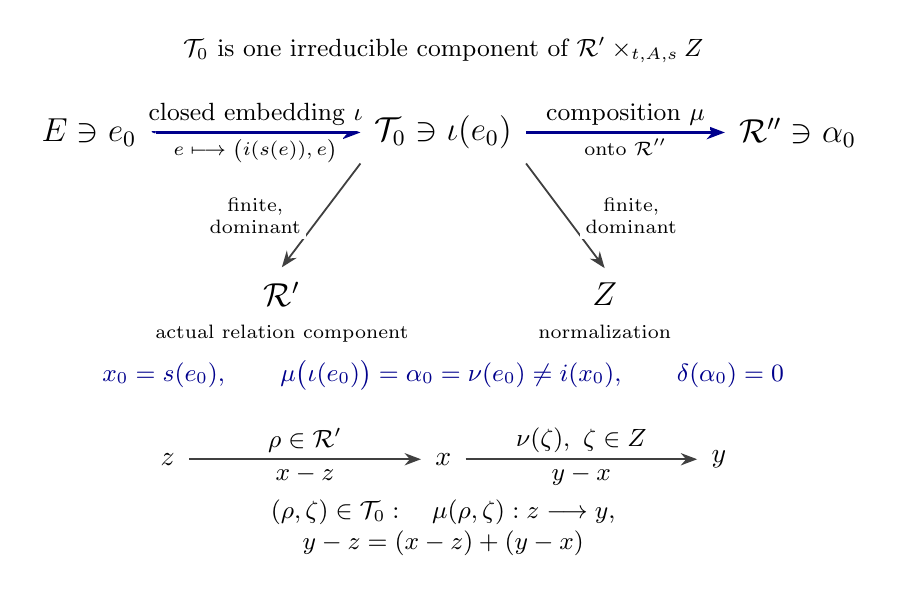
\begin{tikzpicture}[
  >=Stealth,
  object/.style={font=\large, inner sep=5pt, align=center},
  explanation/.style={font=\small, align=center},
  maplabel/.style={font=\small, fill=white, inner sep=2pt},
  retained/.style={draw=blue!55!black, line width=.8pt},
  projection/.style={draw=black!75, line width=.65pt}
]
  \node[object] (E) at (-4.5,0) {$E\ni e_0$};
  \node[object] (T) at (0,0) {$\mathcal T_0\ni\iota(e_0)$};
  \node[object] (Rpp) at (4.5,0) {$\mathcal R''\ni\alpha_0$};

  \node[explanation] at (0,1.05)
    {$\mathcal T_0$ is one irreducible component of
     $\mathcal R'\times_{t,A,s}Z$};

  \draw[retained,{Hooks[right]}->] (E.east) -- (T.west)
    node[midway,above,maplabel] {closed embedding $\iota$}
    node[midway,below,maplabel,font=\scriptsize]
      {$e\longmapsto\bigl(i(s(e)),e\bigr)$};
  \draw[retained,->] (T.east) -- (Rpp.west)
    node[midway,above,maplabel] {composition $\mu$}
    node[midway,below,maplabel,font=\scriptsize] {onto $\mathcal R''$};

  \node[object] (Rp) at (-2.05,-2.05) {$\mathcal R'$};
  \node[object] (Z) at (2.05,-2.05) {$Z$};
  \draw[projection,->] (T.south west) -- (Rp.north)
    node[midway,left=5pt,maplabel,font=\scriptsize,align=center]
      {finite,\\dominant};
  \draw[projection,->] (T.south east) -- (Z.north)
    node[midway,right=5pt,maplabel,font=\scriptsize,align=center]
      {finite,\\dominant};
  \node[explanation,font=\scriptsize,anchor=north] at (-2.05,-2.32)
    {actual relation component};
  \node[explanation,font=\scriptsize,anchor=north] at (2.05,-2.32)
    {normalization};

  \node[explanation,text=blue!55!black] at (0,-3.08)
    {$x_0=s(e_0),\qquad
      \mu\bigl(\iota(e_0)\bigr)=\alpha_0=\nu(e_0)\ne i(x_0),
      \qquad\delta(\alpha_0)=0$};

  \node[object,font=\normalsize] (source) at (-3.5,-4.15) {$z$};
  \node[object,font=\normalsize] (middle) at (0,-4.15) {$x$};
  \node[object,font=\normalsize] (target) at (3.5,-4.15) {$y$};
  \draw[projection,->] (source.east) -- (middle.west)
    node[midway,above,maplabel] {$\rho\in\mathcal R'$}
    node[midway,below,maplabel] {$x-z$};
  \draw[projection,->] (middle.east) -- (target.west)
    node[midway,above,maplabel] {$\nu(\zeta),\ \zeta\in Z$}
    node[midway,below,maplabel] {$y-x$};
  \node[explanation] at (0,-5.02)
    {$(\rho,\zeta)\in\mathcal T_0:\quad
      \mu(\rho,\zeta):z\longrightarrow y,$\\
      $y-z=(x-z)+(y-x)$};
\end{tikzpicture}
\caption{The component used for composition.  The whole divisor
\(E\), including \(e_0\), lies in one component \(\mathcal T_0\) whose
two finite projections are dominant.  Along \(E\) the first arrow is
the identity, so composition retains \(\nu(E)\) and the marked
nonidentity arrow \(\alpha_0\).  The bottom row shows how the two
differences add: dominance onto \(\mathcal R'\) supplies a difference
outside \(D\), while the second difference lies in \(D\).}
\label{quot:incidence}
\end{figure}

Thus every stabilizer is trivial.  A Deligne--Mumford stack
with trivial inertia is an algebraic space, and its coarse morphism
is then an isomorphism.  Therefore \(\mathfrak B=B\), and \(B\) is smooth.
\end{proof}

\section{Completion of the proof}\label{sec:conclusion}

\begin{proof}[Proof of Theorem~\ref{thm:main}]
The case $n=1$ was settled in Section~\ref{sec:setup}; assume $n>1$.
By Lemma~\ref{lem:betti-bound}, $b_2(X)\geq4$.
If \(b_2(X)\geq5\), Proposition~\ref{def:large-betti} gives quotient
singularities for \(B\). If \(b_2(X)=4\) and the polarized family of
smooth fibers of the original \(f\) is isotrivial,
Proposition~\ref{iso:exclusion} gives the same conclusion.
In the remaining case, Proposition~\ref{secsys:rank-four-variation}
chooses the two systems of Proposition~\ref{secsys:second-system} on a
projective IHS deformation \(X'\), still with \(b_2(X')=4\):
projective Lagrangian fibrations \(f':X'\to B\) and \(g:X'\to C\), with
\(C\) normal and projective, such that \(g\) has nonzero polarized
variation and \(f'\) restricts to a finite surjection on every smooth
fiber of \(g\).
If \(B\) had a nonquotient germ, a maximal chart would be singular.
Propositions~\ref{str:minimum} and~\ref{str:products} would supply the
fixed stratum \((S_0,\cS)\) and its product presentations.
Proposition~\ref{eu:euler-zero}, applied to the original fibration,
would give \(\chi_{\mathrm{top}}(S_0)=0\).
For the two fibrations on \(X'\), Proposition~\ref{var:exclusion}
instead gives \(\chi_{\mathrm{top}}(S_0)>0\), a contradiction.
Thus every germ of \(B\) is a quotient singularity in this case as well.
The three cases exhaust the possibilities.

Using the fixed-base family, Proposition~\ref{secsys:second-system}
supplies in every case a finite cover of the unchanged \(B\) by an
\(n\)-dimensional abelian variety:
restrict its first fibration to a smooth fiber of the second.
This cover, the quotient singularities just proved, and the original
projective fibration \(f:X\to B\) meet the hypotheses of
Proposition~\ref{quot:smooth-base}. Hence \(B\) is smooth.
The original $X$ is projective, $f$ is surjective with connected
positive-dimensional fibers, and $B$ is now smooth and projective.
Hwang's theorem applies with precisely these hypotheses
\cite[Theorem~1.2, in the setting of Theorem~1.1]{Hwang2008}, giving
$B\simeq\PP^n_{\C}$.
\end{proof}

\bibliographystyle{plain}
\bibliography{references}
\end{document}
